\documentclass[xcolor={table}]{beamer}
\usepackage{fleqn}
\usepackage{graphicx}
\usepackage{coordsys} %for \numbline commander

%Setup appearance:
\usetheme{Darmstadt}
\usefonttheme[onlylarge]{structurebold}
\setbeamerfont*{frametitle}{size=\normalsize,series=\bfseries}
\setbeamertemplate{navigation symbols}{}
\setbeamertemplate{bibliography item}{[\theenumiv]}

% Standard packages
\usepackage[english]{babel}
\usepackage[latin1]{inputenc}
\usepackage{times}
\usepackage[T1]{fontenc}
\usepackage{multirow}
\usepackage{subfigure}
\usepackage{pbox}
\usepackage{arydshln}
\usepackage{pifont}
\usepackage{cancel}
\usepackage{rotating} % for sideways headings

% Source Code packages
\usepackage{algorithm2e}
\usepackage{algorithmic}

\DeclareSymbolFont{extraup}{U}{zavm}{m}{n}
\DeclareMathSymbol{\varclub}{\mathalpha}{extraup}{84}
\DeclareMathSymbol{\varspade}{\mathalpha}{extraup}{85}
\DeclareMathSymbol{\varheart}{\mathalpha}{extraup}{86}
\DeclareMathSymbol{\vardiamond}{\mathalpha}{extraup}{87}

%%% This section command that adds a big page with section dividers
\usepackage{xifthen}% provides \isempty test
\newcommand{\SectionSlide}[2][]{
	\ifthenelse{\isempty{#1}}
		{\section{#2}\begin{frame} \begin{center}\begin{huge}#2\end{huge}\end{center}\end{frame}}
		{\section[#1]{#2}\begin{frame} \begin{center}\begin{huge}#2\end{huge}\end{center}\end{frame}}
}
%Extends the section slide to to include a shortened section title for the navigation bar as a second parameter
\newcommand{\SectionSlideShortHeader}[3][]{
	\ifthenelse{\isempty{#1}}
		{\section[#3]{#2}\begin{frame} \begin{center}\begin{huge}#2\end{huge}\end{center}\end{frame}}
		{\section[#1]{#2}\begin{frame} \begin{center}\begin{huge}#3\end{huge}\end{center}\end{frame}}
}

\newcommand{\refer}[1]{\footnote{#1}}
\newcommand{\GW}{\text{\textit{Guess-Who~}}}
\newcommand{\keyword}[1]{\alert{\textbf{#1}}\index{#1}}
\newcommand{\firstkeyword}[1]{\textbf{#1}\index{#1}}
\newcommand{\indexkeyword}[1]{\alert{\textbf{#1}\index{#1}}}
\newcommand{\featN}[1]{\textsc{#1}}
\newcommand{\featL}[1]{\textit{'#1'}}
 \newcommand{\ourRef}[1]{\ref{#1} $^{\text{\tiny[\pageref{#1}]}}$}
 \newcommand{\ourEqRef}[1]{\eqref{#1}$^{\text{\tiny[\pageref{#1}]}}$}
  
\DeclareMathOperator*{\argmax}{argmax}
\DeclareMathOperator*{\argmin}{argmin}
\def\<{\langle}
\def\>{\rangle}


\title{Error-based Learning\\Sections $7.4, 7.5$}
	\author{John D. Kelleher and Brian Mac Namee and Aoife D'Arcy}
	\institute{}
	\date{}

\begin{document}
\begin{frame}
	\titlepage
\end{frame}
\begin{frame}
	 \tableofcontents
\end{frame}


\SectionSlideShortHeader{Interpreting Multivariable Linear Regression Models}{Interpreting}

\begin{frame}
\begin{itemize}
\item The weights used by linear regression models indicate the effect of each descriptive feature on the predictions returned by the model. 
\item Both the \keyword{sign} and the \keyword{magnitude} of the weight provide information on how the descriptive feature effects the predictions of the model.
\end{itemize}

\begin{table}[!hbt]
	\caption{Weights and standard errors for each feature in the office rentals model.}
	\centering
	\begin{footnotesize}
	\begin{tabular}{ l r r r r }
		\hline
		Descriptive Feature & Weight & Standard Error & \textit{t}-statistic & \textit{p}-value \\
		\hline
		\featN{Size} & 0.6270	&	0.0545	&	11.504	& $<$0.0001	\\
		\featN{Floor} & -0.1781	&	2.7042		& -0.066	& 0.949	\\
		\featN{Broadband Rate} &	0.071396	& 0.2969	& 0.240	& 0.816	\\
		\hline
	\end{tabular}
	\end{footnotesize}
\label{tab:modelEffectsOfficeRentals}
\end{table}
\end{frame} 



\begin{frame}
\begin{itemize}
\item It is tempting to infer the relative  importance of the different descriptive features in the model from the magnitude of the weights
\item However, direct comparison of the weights tells us little about their relative importance.
\item A better way to determine the importance of each descriptive feature in the model is to perform a \keyword{statistical significance test}.
\end{itemize}
\end{frame} 

 \begin{frame} 
 \begin{itemize}
 \item The statistical significance test we use to analyze the importance of a descriptive feature $\mathbf{d}\left[j\right]$ in a linear regression model is the \keyword{\textit{t}-test}.
\item The null hypothesis for this test is that the feature does not have a significant impact on the model. The test statistic we calculate is called the \textit{t}-statistic.
\end{itemize}
\end{frame}

\begin{frame}
\begin{itemize}
\item The standard error for the overall model is calculated as
\begin{equation}
se = \sqrt{\frac{\displaystyle \sum_{i=1}^{n} \left( t_i - \mathbb{M}_{\mathbf{w}}(\mathbf{d}_i) \right)^2}{n - 2}} \label{eqn:standardError}
\end{equation}
\item A standard error calculation is then done for a descriptive feature as follows:
\begin{equation}
se(\mathbf{d}\left[j\right])  =  \frac{se}{\sqrt{\displaystyle \sum_{i=1}^{n} \left( \mathbf{d}_i\left[j\right] - \overline{\mathbf{d}\left[j\right]} \right)^2}} 
\label{eqn:descriptivefeatureStandardError}
\end{equation}
\item The \textit{t}-statistic for this test is calculated as follows:
\begin{eqnarray}
t & = & \frac{\mathbf{w}\left[j\right]}{se\left(\mathbf{d}\left[j\right]\right)} \label{eqn:tStat}
\end{eqnarray}
\end{itemize}
\end{frame} 


\begin{frame}
\begin{itemize}
\item Using a standard \textit{t}-statistic look-up table, we can then determine the \textit{p}-value associated with this test (this is a two tailed \textit{t}-test with degrees of freedom set to the number of instances in the training set minus $2$). 
\item If the \textit{p}-value is less than the required significance level, typically $0.05$, we reject the null hypothesis and say that the descriptive feature has a significant impact on the model; otherwise we say that it does not. 
\end{itemize}
\begin{table}[!hbt]
	\caption{Weights and standard errors for each feature in the office rentals model.}
	\centering
	\begin{footnotesize}
	\begin{tabular}{ l r r r r }
		\hline
		Descriptive Feature & Weight & Standard Error & \textit{t}-statistic & \textit{p}-value \\
		\hline
		\featN{Size} & 0.6270	&	0.0545	&	11.504	& $<$0.0001	\\
		\featN{Floor} & -0.1781	&	2.7042		& -0.066	& 0.949	\\
		\featN{Broadband Rate} &	0.071396	& 0.2969	& 0.240	& 0.816	\\
		\hline
	\end{tabular}
	\end{footnotesize}
\label{tab:modelEffectsOfficeRentals}
\end{table}
\end{frame} 


\SectionSlideShortHeader{Setting the Learning Rate Using Weight Decay}{Learning Rate}



 \begin{frame} 
 \begin{itemize}
 \item \keyword{Learning rate decay} allows the learning rate to start at a large value and then decay over time according to a predefined schedule. 
 \item A good approach is to use the following decay schedule:
\begin{eqnarray}
	\alpha_\tau & = & \alpha_0\frac{c}{c + \tau}
	\label{eqn:learningRateDecay}
\end{eqnarray}
\end{itemize}
\end{frame} 

 \begin{frame} 
\begin{figure}[!htb]
\begin{center}
	\subfigure[]{\label{fig:learningRatesWithDecayErrorSurface}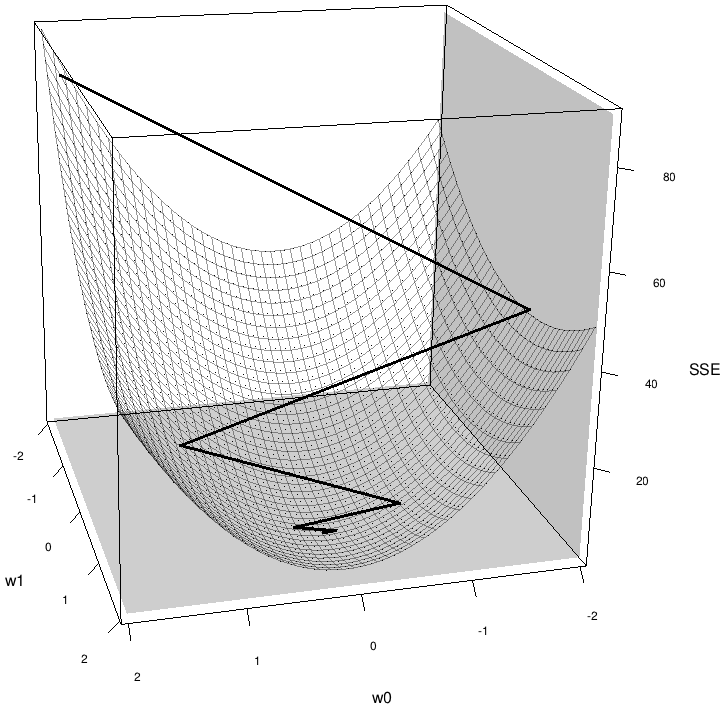
\includegraphics[width=0.4\textwidth]{./images/linearRegressionDemoErrorSurfaceJourneyLearningRateDecay0_18-10.png}}
	\subfigure[]{\label{fig:learningRatesWithDecayErrorGraph}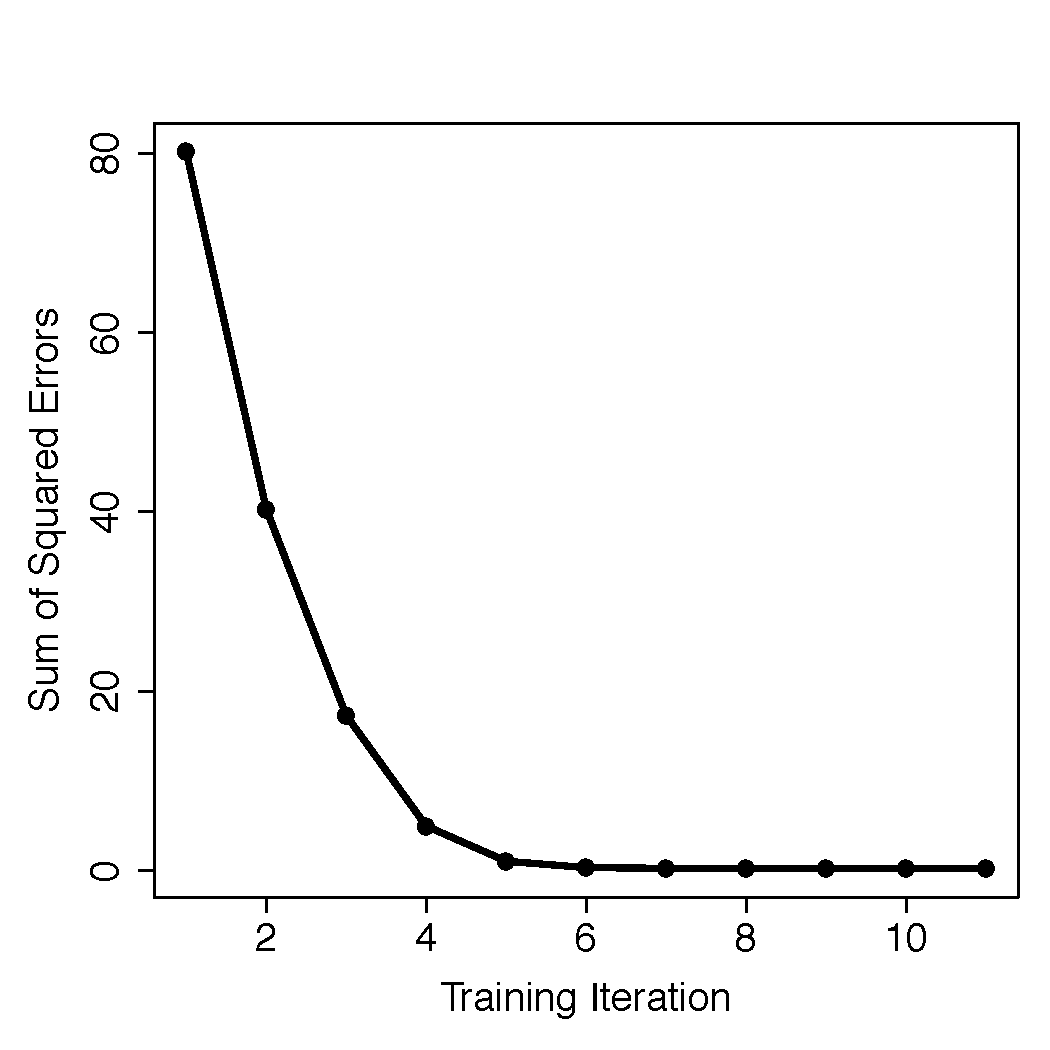
\includegraphics[width=0.4\textwidth]{./images/linearRegressionDemoErrorJourneyLearningRateDecay0_18-10.pdf}}
\caption{(a) The journey across the error surface for the office rentals prediction problem when learning rate decay is used ($\alpha_0 = 0.18$, $c = 10$ ); (b) a plot of the changing sum of squared error values during this journey. }
\label{fig:learningRatesWithDecay}
\end{center}
\end{figure}
\end{frame} 

 \begin{frame} 
\begin{figure}[!thb]
\begin{center}
	\subfigure[]{\label{fig:learningRatesWithDecayErrorSurfaceExample2}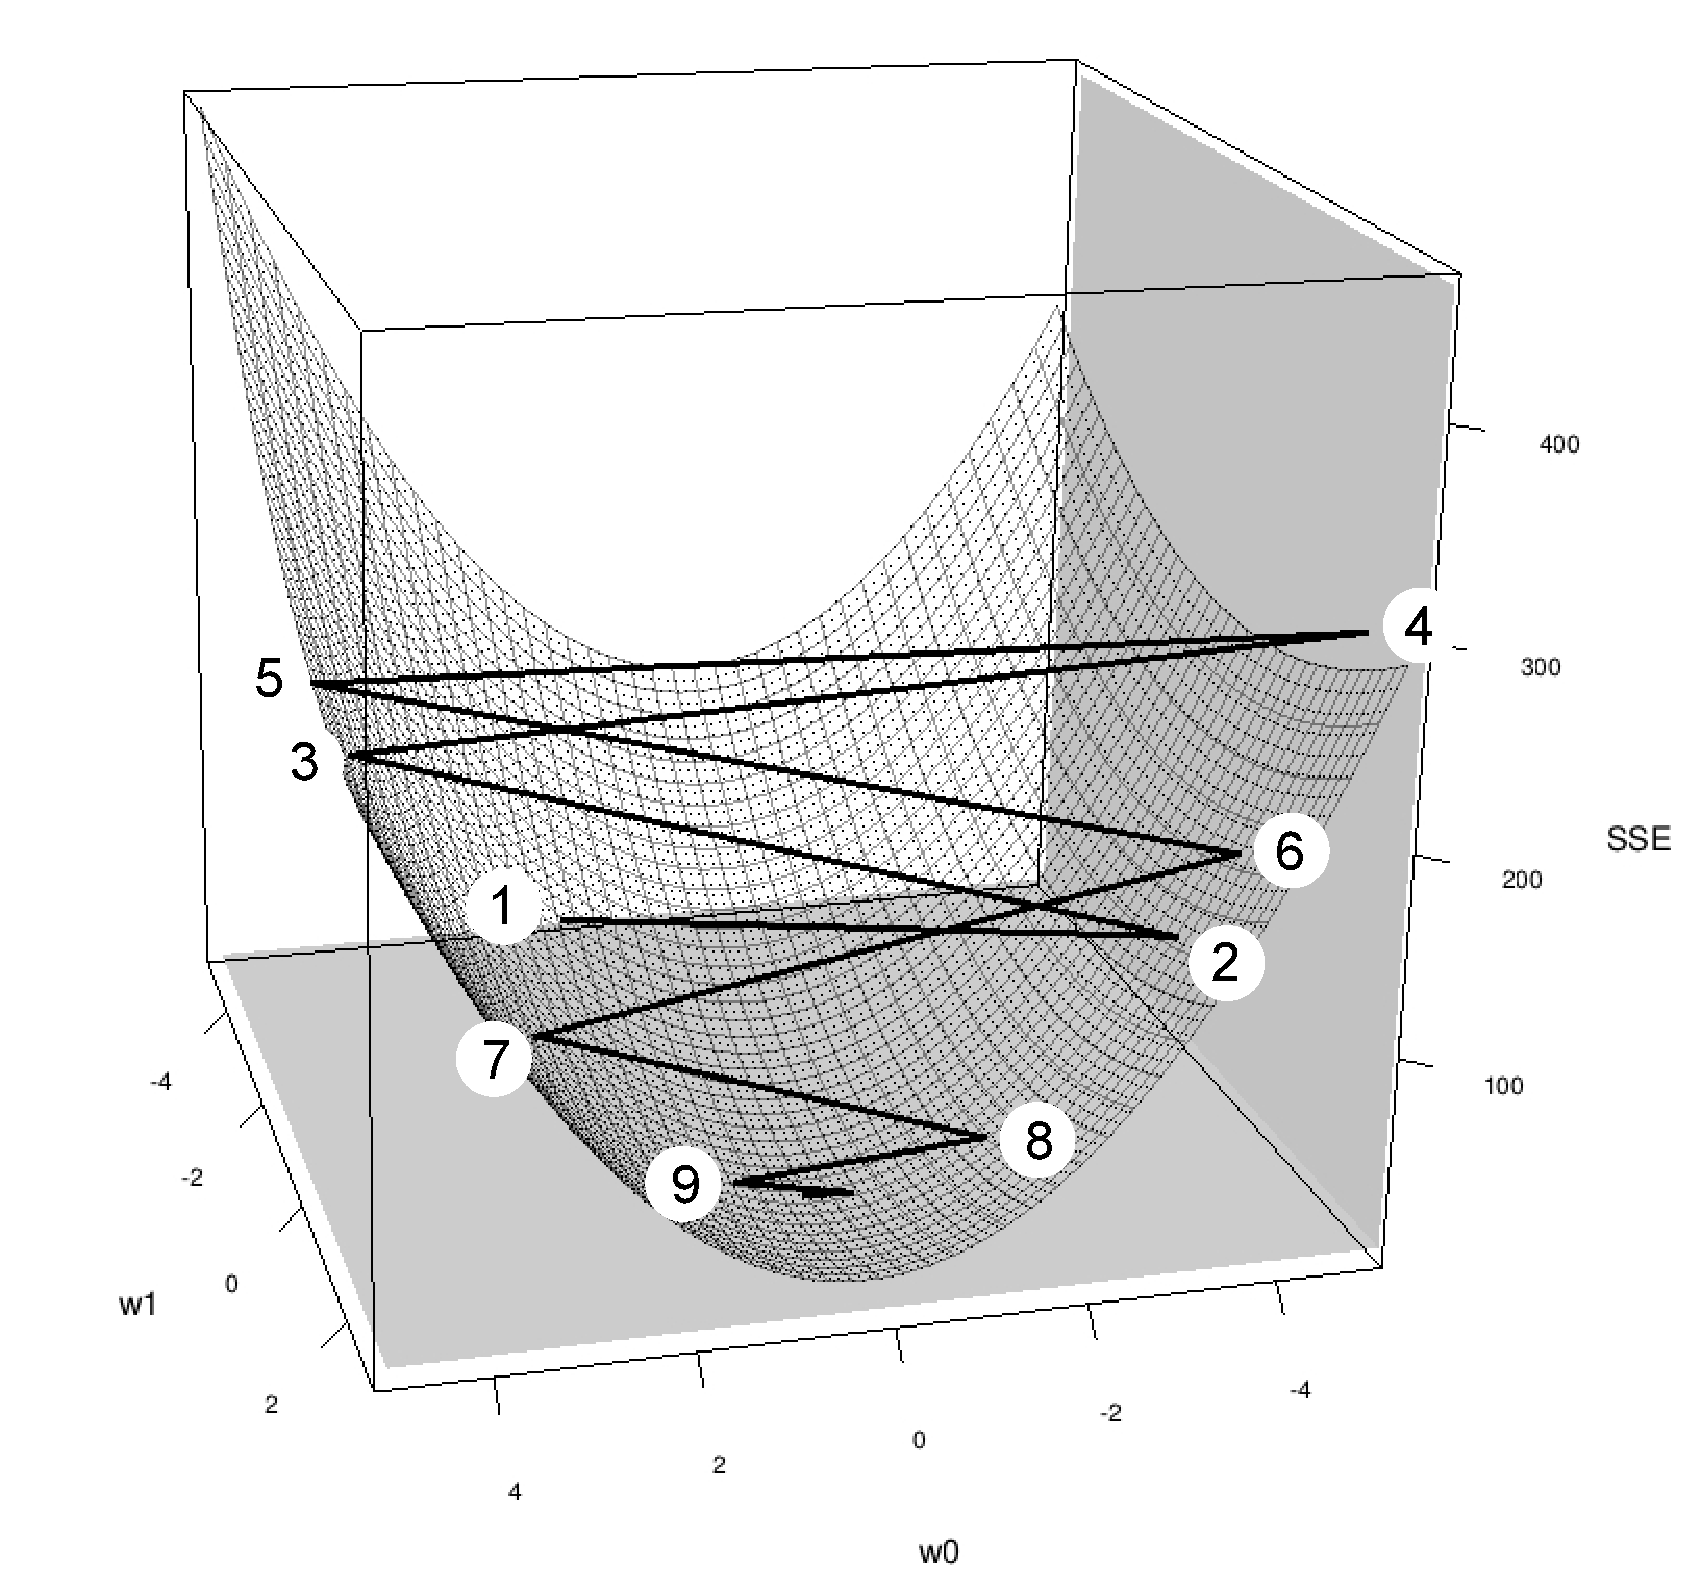
\includegraphics[width=0.4\textwidth]{./images/linearRegressionDemoErrorSurfaceJourneyLearningRateDecay0_25-100.pdf}}
	\subfigure[]{\label{fig:learningRatesWithDecayErrorGraphExample2}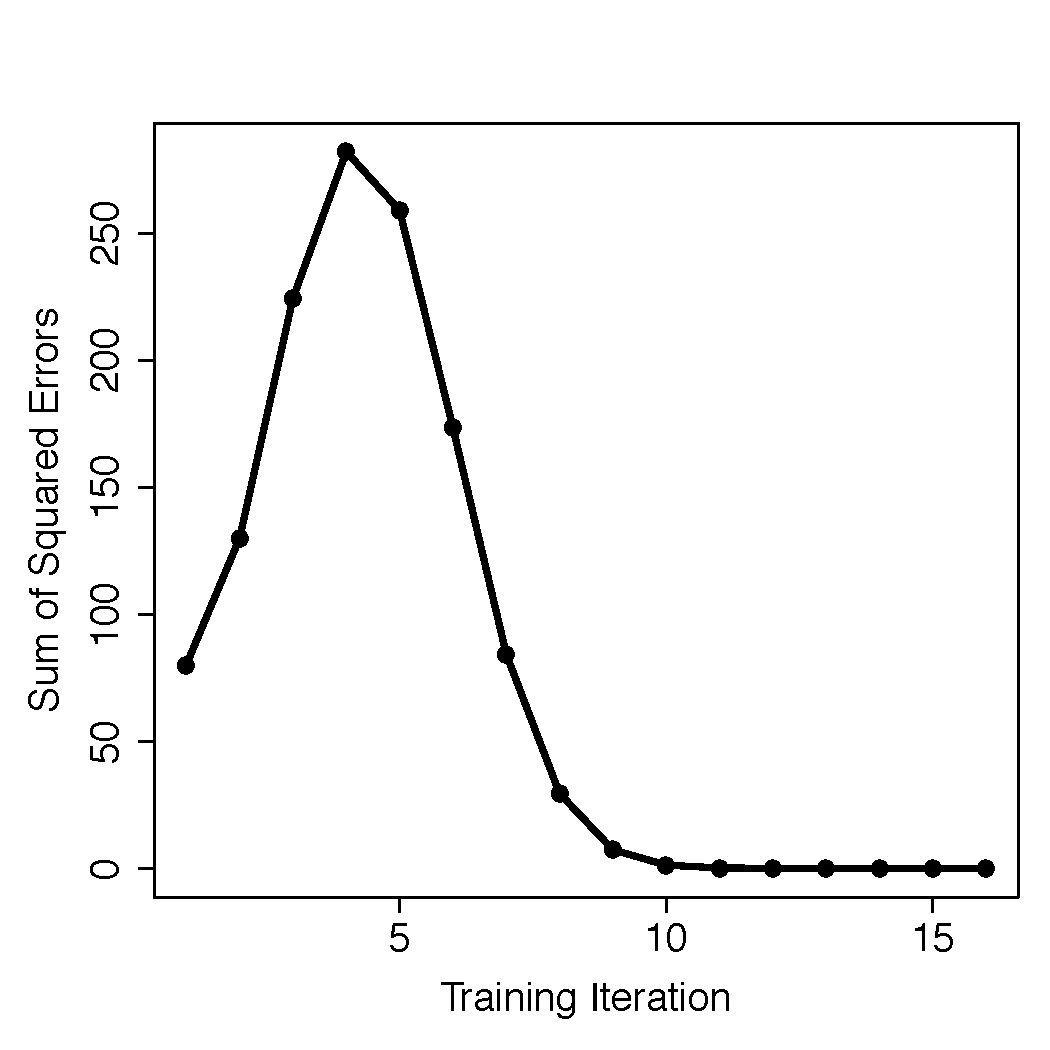
\includegraphics[width=0.4\textwidth]{./images/linearRegressionDemoErrorJourneyLearningRateDecay0_25-100.pdf}}

\caption{(a) The journey across the error surface for the office rentals prediction problem when learning rate decay is used ($\alpha_0 = 0.25$, $c = 100$); (b) a plot of the changing sum of squared error values during this journey. }
\label{fig:learningRatesWithDecayExample2}
\end{center}
\end{figure}
\end{frame} 


\SectionSlideShortHeader{Handling Categorical Descriptive Features}{Cat. Features}

 \begin{frame} 
 \begin{itemize}
\item The basic structure of the multivariable linear regression model allows for only continuous descriptive features, so we need a way to handle categorical descriptive features. 
\item The most common approach to handling categorical features uses a transformation that converts a single categorical descriptive feature into a number of continuous descriptive feature values that can encode the levels of the categorical feature. 
\item For example, the \featN{Energy Rating} descriptive feature would be converted into three new continuous descriptive features, as it has 3 distinct levels: \featL{A}, \featL{B}, or \featL{C}. 
\end{itemize}
\end{frame} 

 \begin{frame} 
\begin{table}
	\caption{The office rentals dataset adjusted to handle the categorical \featN{Energy Rating} descriptive feature in linear regression models.}
	\centering
	\resizebox{\textwidth}{!}{
			\begin{footnotesize}
	\begin{tabular}{ c c c c c c c c }
		\hline
				~	 & ~	 & ~ & \featN{Broadband} & \featN{Energy} & \featN{Energy} & \featN{Energy} & \featN{Rental}\\
				\featN{ID}	 & \featN{Size} & \featN{Floor} & \featN{Rate} & \featN{Rating A} & \featN{Rating B} & \featN{Rating C} & \featN{Price}\\
		\hline
1	&	500	&	4	&	8	&	0	& 0 & 1 &	320	\\
2	&	550	&	7	&	50	&	1	& 0 & 0 &	380	\\
3	&	620	&	9	&	7	&	1	& 0 & 0	&	400	\\
4	&	630	&	5	&	24	&	0	& 1 & 0	&	390	\\
5	&	665	&	8	&	100	&	0	& 0 & 1	&	385	\\
6	&	700	&	4	&	8	&	0	& 1 & 0	&	410	\\
7	&	770	&	10	&	7	&	0	& 1 & 0	&	480	\\
8	&	880	&	12	&	50	&	1	& 0 & 0	&	600	\\
9	&	920	&	14	&	8	&	0	& 0 & 1	&	570	\\
10	&	1\,000	&	9	&	24	&	0	& 1 & 0	&	620	\\
		\hline
	\end{tabular}
			\end{footnotesize}
			}
\label{tab:officeSizesAndPricesCategoricalConvert}
\end{table}
\end{frame} 



 \begin{frame} 
 \begin{itemize}
\item Returning to our example, the regression equation for this \featN{Rental Price} model would change to
\begin{eqnarray*}
	\featN{Rental Price} =  \mathbf{w}\left[0\right] 	& + &  \mathbf{w}\left[1\right] \times \featN{Size} + \mathbf{w}\left[2\right] \times \featN{Floor}	\\
													& + &  \mathbf{w}\left[3\right] \times \featN{Broadband~Rate} \\
													& + &  \mathbf{w}\left[4\right] \times \featN{Energy~Rating~A} \\
													& + &  \mathbf{w}\left[5\right] \times  \featN{Energy~Rating~B} \\
 													& + &  \mathbf{w}\left[6\right] \times \featN{Energy~Rating~C}
\end{eqnarray*}
\noindent where the newly added categorical features allow the original \featN{Energy Rating} feature to be included. 
\end{itemize}
\end{frame} 


\SectionSlideShortHeader{Handling Categorical Target Features: Logistic Regression}{Logistic Reg.}

 \begin{frame} [plain]
\begin{table}[!bht]
	\caption{A dataset listing features for a number of generators.}
\label{tab:faultyMachineryData}
\centering
\begin{tiny}
\begin{tabular}{cc}
		\hline
			\begin{minipage}{0.48\textwidth}
					\begin{tabular}[ht]{ c c c c }
\featN{ID} & \featN{RPM} & \featN{Vibration} & \featN{Status} \\
		\hline
1	&	568	&	585	&	good	\\
2	&	586	&	565	&	good		\\
3	&	609	&	536	&	good		\\
4	&	616	&	492	&	good		\\
5	&	632	&	465	&	good		\\
6	&	652	&	528	&	good		\\
7	&	655	&	496	&	good		\\
8	&	660	&	471	&	good		\\
9	&	688	&	408	&	good		\\
10	&	696	&	399	&	good		\\
11	&	708	&	387	&	good		\\
12	&	701	&	434	&	good		\\
13	&	715	&	506	&	good		\\
14	&	732	&	485	&	good		\\
15	&	731	&	395	&	good		\\
16	&	749	&	398	&	good		\\
17	&	759	&	512	&	good		\\
18	&	773	&	431	&	good		\\
19	&	782	&	456	&	good		\\
20	&	797	&	476	&	good		\\
21	&	794	&	421	&	good		\\
22	&	824	&	452	&	good		\\
23	&	835	&	441	&	good		\\
24	&	862	&	372	&	good		\\
25	&	879	&	340	&	good		\\
26	&	892	&	370	&	good		\\
27	&	913	&	373	&	good		\\
28	&	933	&	330	&	good	\\
		\hline
					\end{tabular}
			\end{minipage}
			&
			\begin{minipage}{0.48\textwidth}
										\begin{tabular}[ht]{ c c c c }
\featN{ID} & \featN{RPM} & \featN{Vibration} & \featN{Status} \\
		\hline
	29	&	562	&	309	&	faulty	\\
30	&	578	&	346	&	faulty	\\
	31	&	593	&	357	&	faulty	\\
	32	&	626	&	341	&	faulty	\\
	33	&	635	&	252	&	faulty	\\
	34	&	658	&	235	&	faulty	\\
35	&	663	&	299	&	faulty	\\
36	&	677	&	223	&	faulty	\\
37	&	685	&	303	&	faulty	\\
38	&	698	&	197	&	faulty	\\
39	&	699	&	311	&	faulty	\\
40	&	712	&	257	&	faulty	\\
41	&	722	&	193	&	faulty	\\
42	&	735	&	259	&	faulty	\\
	43	&	738	&	314	&	faulty	\\
44	&	753	&	113	&	faulty	\\
45	&	767	&	286	&	faulty	\\
46	&	771	&	264	&	faulty	\\
47	&	780	&	137	&	faulty	\\
48	&	784	&	131	&	faulty	\\
49	&	798	&	132	&	faulty	\\
50	&	820	&	152	&	faulty	\\
51	&	834	&	157	&	faulty	\\
52	&	858	&	163	&	faulty	\\
53	&	888	&	91	&	faulty	\\
54	&	891	&	156	&	faulty	\\
55	&	911	&	79	&	faulty	\\
56	&	939	&	99	&	faulty	\\
\hline
				\end{tabular}
			\end{minipage}\\
\end{tabular}
\end{tiny}
\end{table}
\end{frame} 

 \begin{frame} [plain]
\begin{figure}[htb]
\begin{center}
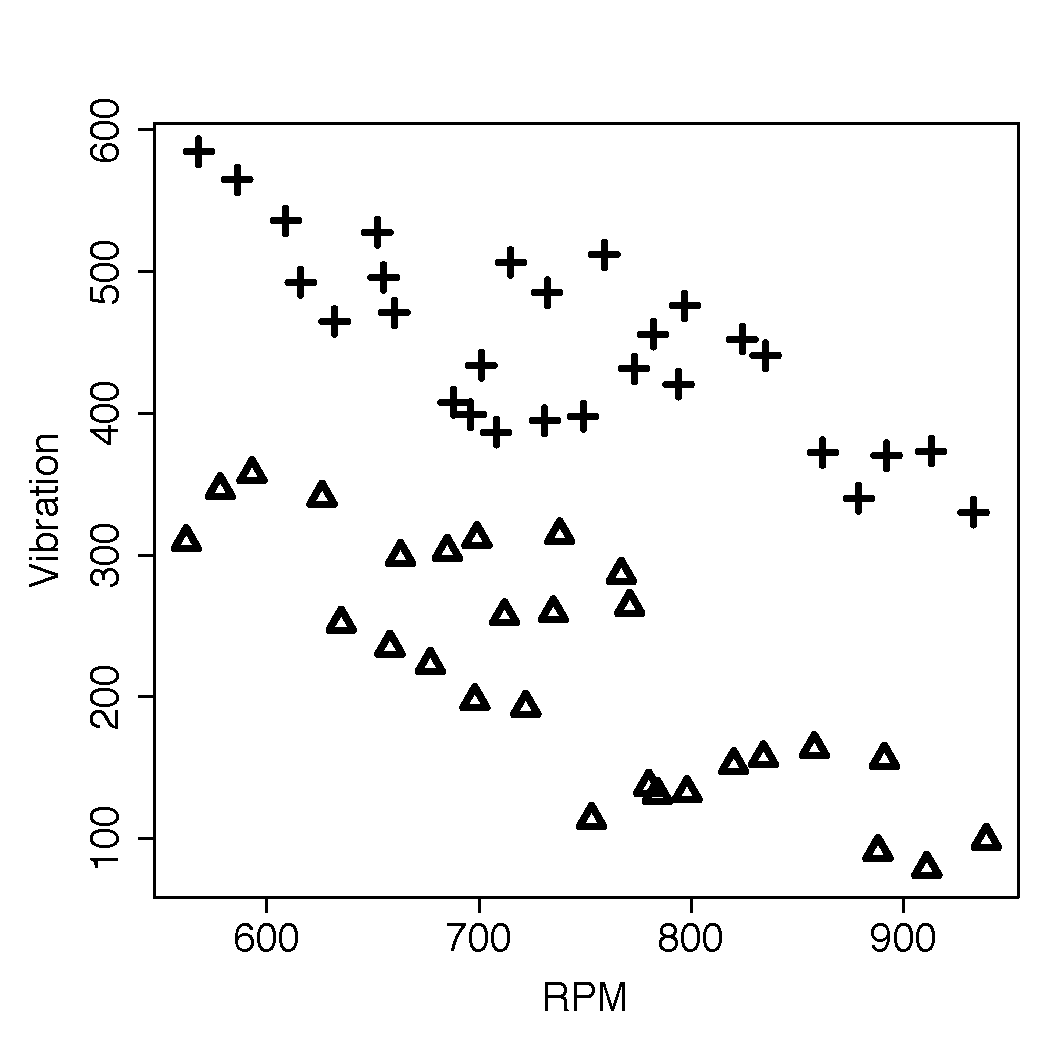
\includegraphics[width=0.65\textwidth]{./images/gradientDescentLogisticClassificationDemoGoodSepNonNormDataset.pdf}
\caption{A scatter plot of the \featN{RPM} and \featN{Vibration} descriptive features from the generators dataset shown in Table \ourRef{tab:faultyMachineryData} where \featL{good} generators are shown as crosses and \featL{faulty} generators are shown as triangles.}
\label{fig:faultyMachinesData}
\end{center}
\end{figure}		
\end{frame} 

 \begin{frame}[plain]
\begin{figure}[htb]
\begin{center}
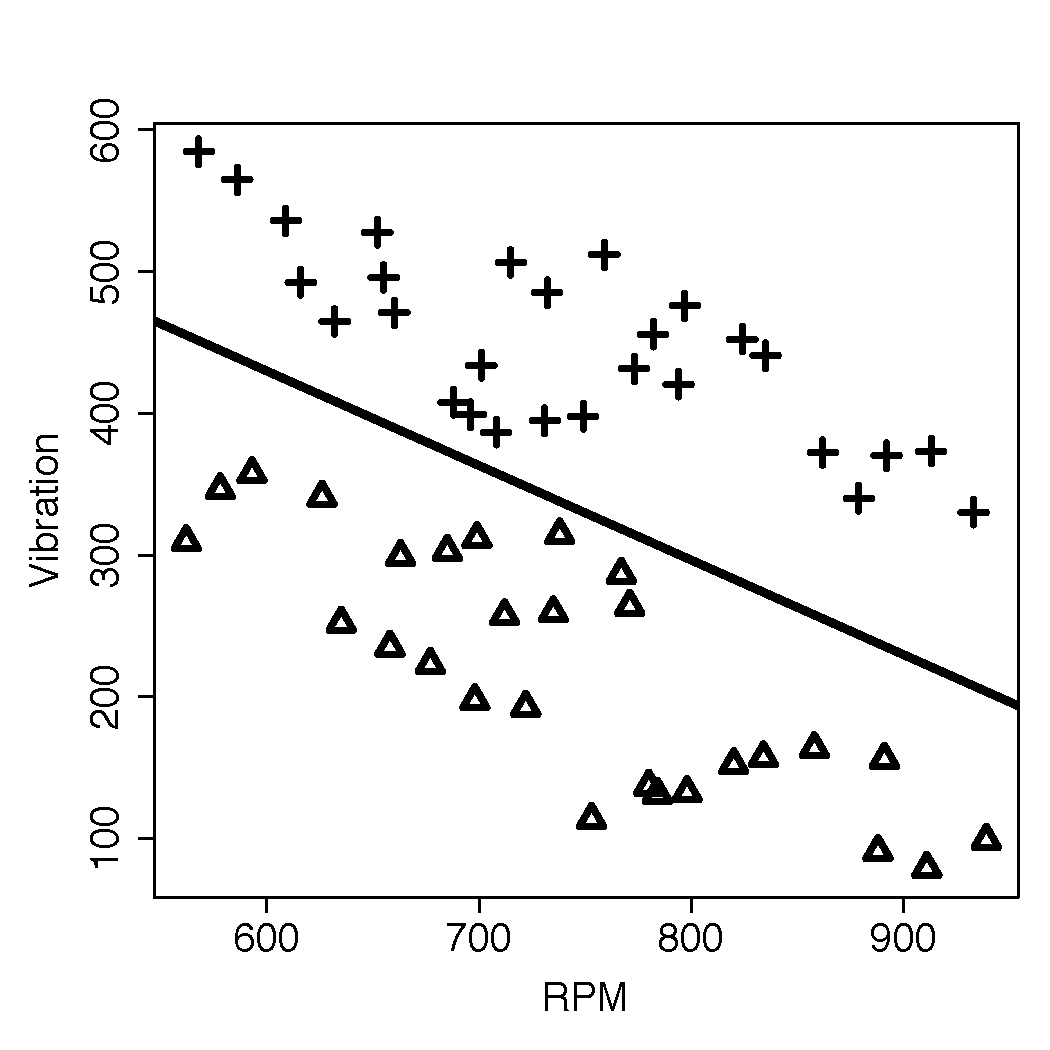
\includegraphics[width=0.65\textwidth]{./images/gradientDescentLogisticClassificationGoodSepNonNormDemoFinal.pdf}
\caption{A scatter plot of the \featN{RPM} and \featN{Vibration} descriptive features from the generators dataset shown in Table \ourRef{tab:faultyMachineryData}. A decision boundary separating \featL{good} generators (crosses) from \featL{faulty} generators (triangles) is also shown.}
\label{fig:faultyMachinesDataLinearSep}
\end{center}
\end{figure}
\end{frame} 

\begin{frame}
\begin{itemize}
\item As the decision boundary is a \indexkeyword{linear separator} it can be defined using the equation of the line as: 
\begin{equation}
\featN{Vibration} = 830 - 0.667\times \featN{RPM}
\end{equation}
\noindent or
\begin{equation}
830 - 0.667\times \featN{RPM} - \featN{Vibration} = 0
\label{eqn:boundaryExample}
\end{equation}
\end{itemize}
\end{frame} 

 \begin{frame} 
 \begin{itemize}
\item Applying Equation \ourEqRef{eqn:boundaryExample} to the instance $\featN{RPM} = 810$, $\featN{Vibration} = 495$, which is be above the decision boundary, gives the following result:
\begin{equation*}
830 - 0.667\times 810 - 495 = -205.27
\end{equation*}
\item By contrast, if we apply Equation \ourEqRef{eqn:boundaryExample} to the instance $\featN{RPM} = 650$ and $\featN{Vibration} = 240$, which is be below the decision boundary, we get 
\begin{equation*}
830 - 0.667\times 650 - 240 = 156.45
\end{equation*}
\end{itemize}
\end{frame} 

\begin{frame}
\begin{itemize}
\item All the data points above the decision boundary will result in a negative value when plugged into the decision boundary equation, while all data points  below the decision boundary will result in a positive value. 
\end{itemize}
\end{frame}

\begin{frame}
\begin{itemize}
\item Reverting to our previous notation we have:
\begin{equation}
\mathbb{M}_{\mathbf{w}}(\mathbf{d}) = 	\begin{cases}
		1 & \text{if } \mathbf{w} \cdot \mathbf{d} \geq 0\\
		0 & otherwise
	\end{cases}
	\label{eqn:classifier}
\end{equation}
\item The surface defined by this rule is known as a \keyword{decision surface}. 
\end{itemize}
\end{frame}

 \begin{frame} 
\begin{figure}[htb]
\begin{center}
\subfigure[]{\label{fig:faultyMachinesDataDecisionSurface}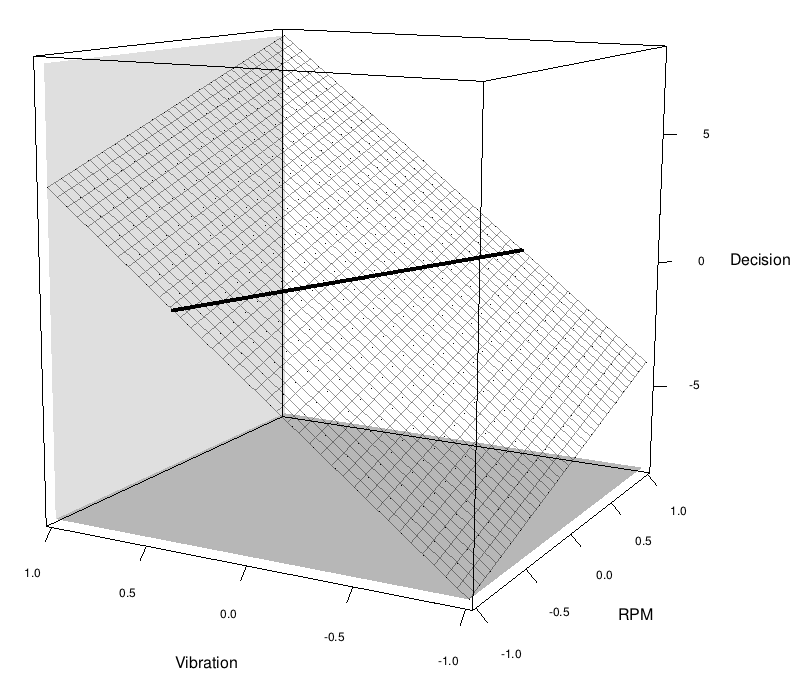
\includegraphics[width=0.49\textwidth]{./images/gradientDescentLogisticClassificationDemoGoodSepNoThreshDecisionSurface.png}}
\subfigure[]{\label{fig:faultyMachinesDataDecisionSurfaceThreshold}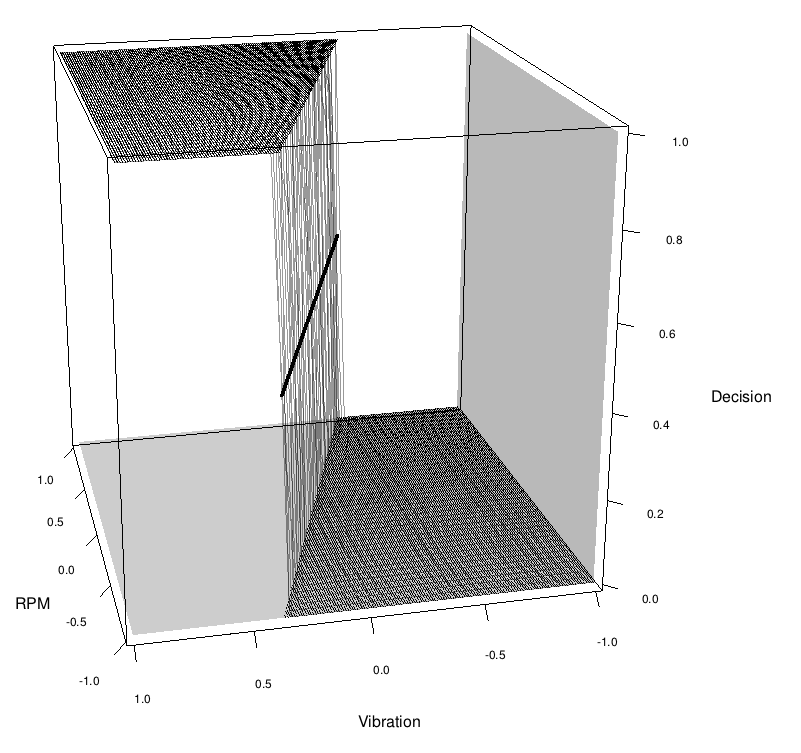
\includegraphics[width=0.49\textwidth]{./images/gradientDescentLogisticClassificationDemoGoodSepLinearThreshDecisionSurface.png}}
\caption{(a) A surface showing the value of Equation \ourEqRef{eqn:boundaryExample} for all values of \featN{RPM} and \featN{Vibration}. The decision boundary given in Equation \ourEqRef{eqn:boundaryExample} is highlighted. (b) The same surface linearly thresholded at zero to operate as a predictor.} 
\label{fig:faultyMachinesDataDecisionSurfaces}
\end{center}
\end{figure}
\end{frame} 

\begin{frame}
\begin{itemize}
\item The hard decision boundary given in Equation \ourEqRef{eqn:classifier} is \indexkeyword{discontinuous} so is not differentiable and so we can't calculate the gradient of the error surface. 
\item Furthermore, the model always makes completely confident predictions of $0$ or $1$, whereas a little more subtlety  is desirable. 
\item We  address these issues by using a more sophisticated threshold function that is continuous, and therefore differentiable, and that allows for the subtlety desired:  the \keyword{logistic function} 
\end{itemize}
\end{frame} 
 
\begin{frame} 
\begin{alertblock}{logistic function}
\begin{eqnarray}
	Logistic(x)=\frac{1}{1+e^{-x}}
	\label{eqn:logisticFunction}
\end{eqnarray}
\noindent where $x$ is a numeric value and $e$ is \indexkeyword{Euler's number} and is approximately equal to $2.7183$.  
\end{alertblock}
\end{frame} 

 \begin{frame} 
\begin{center}
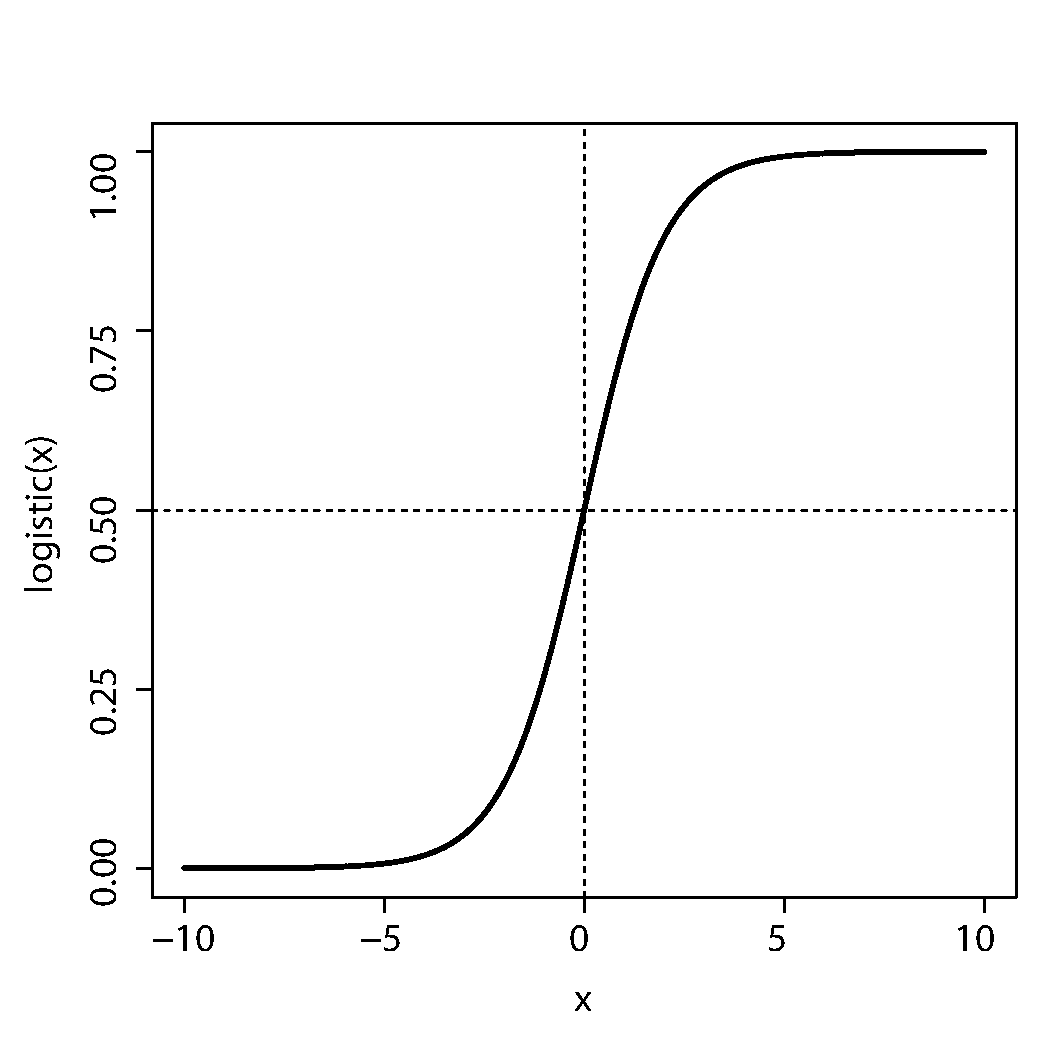
\includegraphics[width=0.8\textwidth]{./images/LogisticFunction.pdf}
\end{center}
\end{frame} 

 \begin{frame} 
 \begin{itemize}
\item  To build a logistic regression model, we simply pass the output of the basic linear regression model through the logistic function 
\end{itemize}
\begin{alignat}{2}
	\mathbb{M}_{\mathbf{w}}(\mathbf{d}) & =  Logistic(\mathbf{w} \cdot \mathbf{d}) \notag \\
	& =  \frac{1}{1+e^{-\mathbf{w} \cdot \mathbf{d}}}
	\label{eqn:logisticRegression}
\end{alignat}

\begin{block}{A note on training logistic regression models:}
\begin{enumerate}
\item Before we train a logistic regression model we map the binary target feature levels to 0 or 1.
\item The error of the model on each instance is then the difference between the target feature (0 or 1) and the value of the prediction $[0,1]$.
\end{enumerate}
\end{block}
\end{frame} 

 \begin{frame} 
 \begin{example}
\begin{alignat*}{2}
		\mathbb{M}_{\mathbf{w}}(&\left< \featN{RPM}, \featN{Vibration} \right>) \notag \\
		& = \frac{1}{1+e^{-(-0.4077 + 4.1697 \times \featN{RPM} + 6.0460 \times \featN{Vibration} )}}
		\label{eqn:faultyMachineryLogisticExample}
\end{alignat*}
\end{example}
\end{frame} 

 \begin{frame} 
\begin{center}
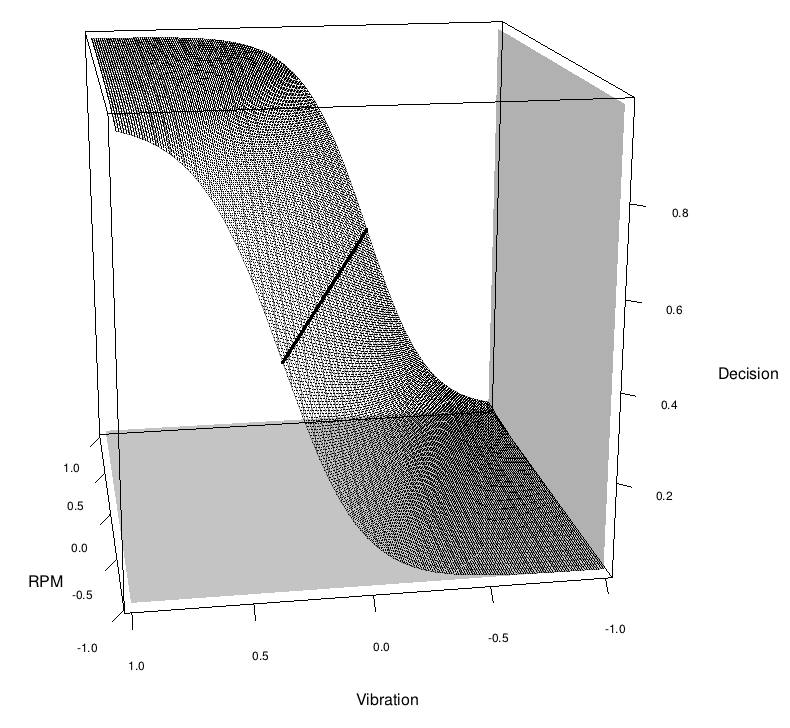
\includegraphics[width=0.6\textwidth]{./images/gradientDescentLogisticClassificationDemoGoodSepLogisticThreshDecisionSurface.png}
\end{center}
 \begin{itemize}
 	\item The decision surface for the example logistic regression model.
\end{itemize}
\end{frame} 

 \begin{frame} 
 \begin{equation*}
 P(t=\featL{faulty} | \mathbf{d}) = \mathbb{M}_{\mathbf{w}}(\mathbf{d})
 \end{equation*}
 \begin{equation*}
P(t=\featL{good} | \mathbf{d}) = 1 - \mathbb{M}_{\mathbf{w}}(\mathbf{d})
 \end{equation*}
\end{frame} 

 \begin{frame} 
\begin{figure}[htb]
\begin{center}
	\subfigure{\label{fig:machineryGoodSepGradientDescentSmallMultiples1}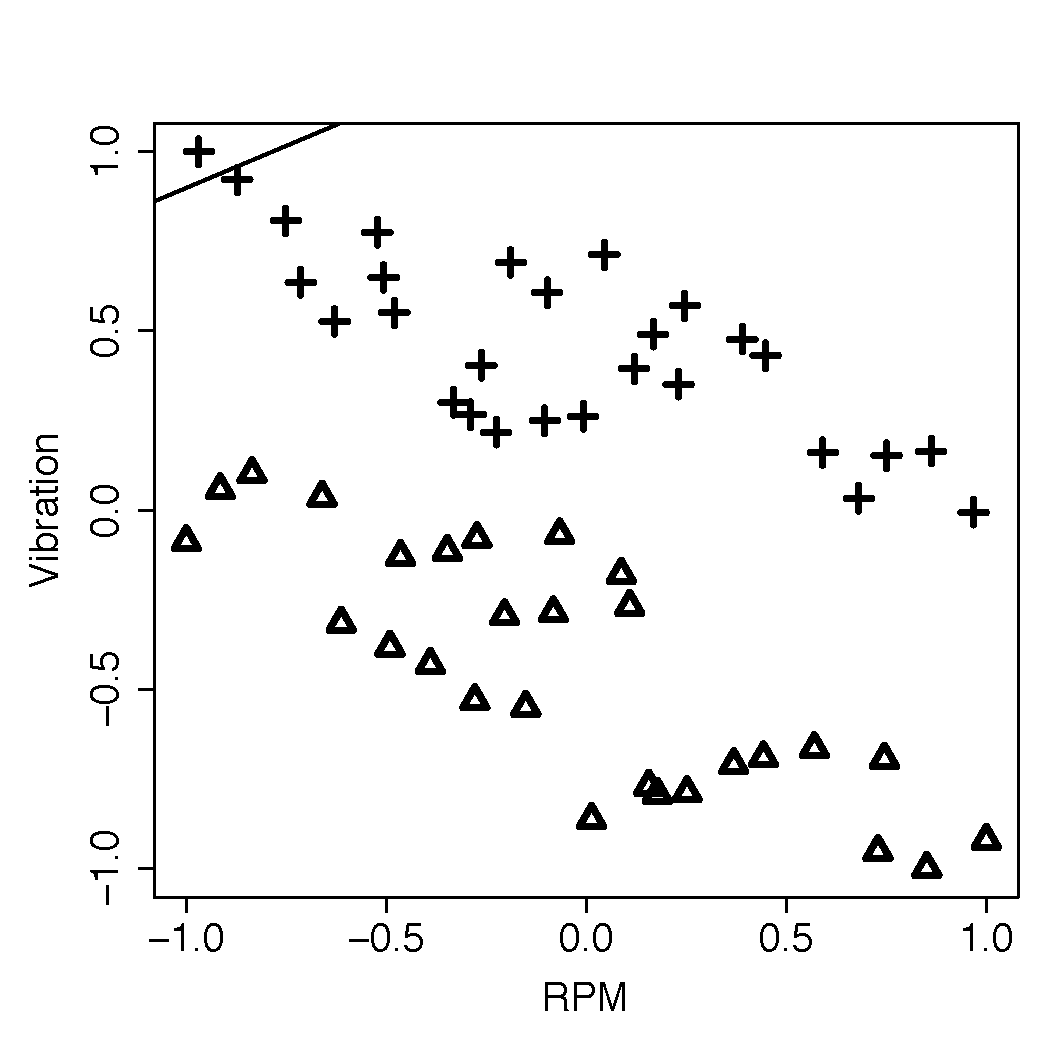
\includegraphics[width=0.27\textwidth]{./images/gradientDescentLogisticClassificationDemoGoodSep0.pdf}}
	\subfigure{\label{fig:machineryGoodSepGradientDescentSmallMultiples3}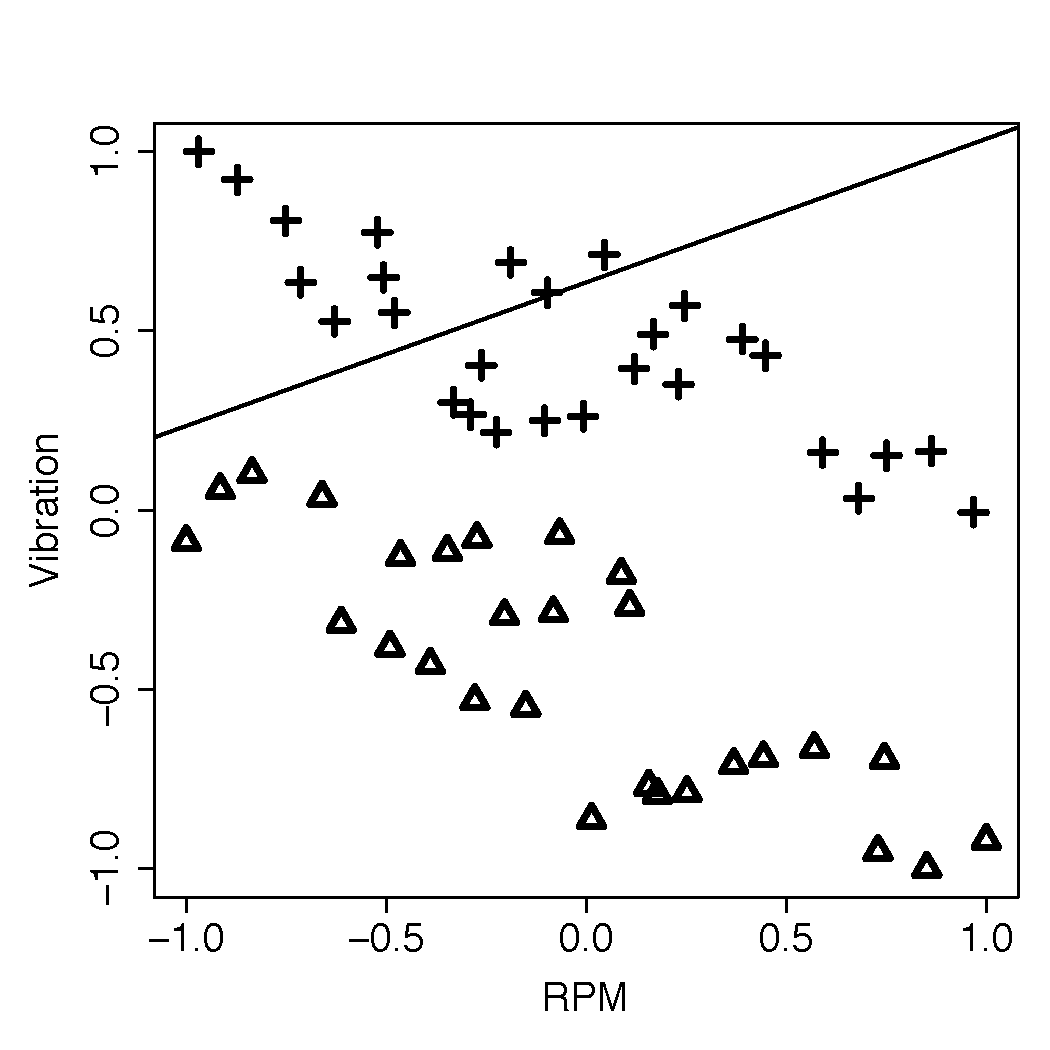
\includegraphics[width=0.27\textwidth]{./images/gradientDescentLogisticClassificationDemoGoodSep22.pdf}}
	\subfigure{\label{fig:machineryGoodSepGradientDescentSmallMultiples5}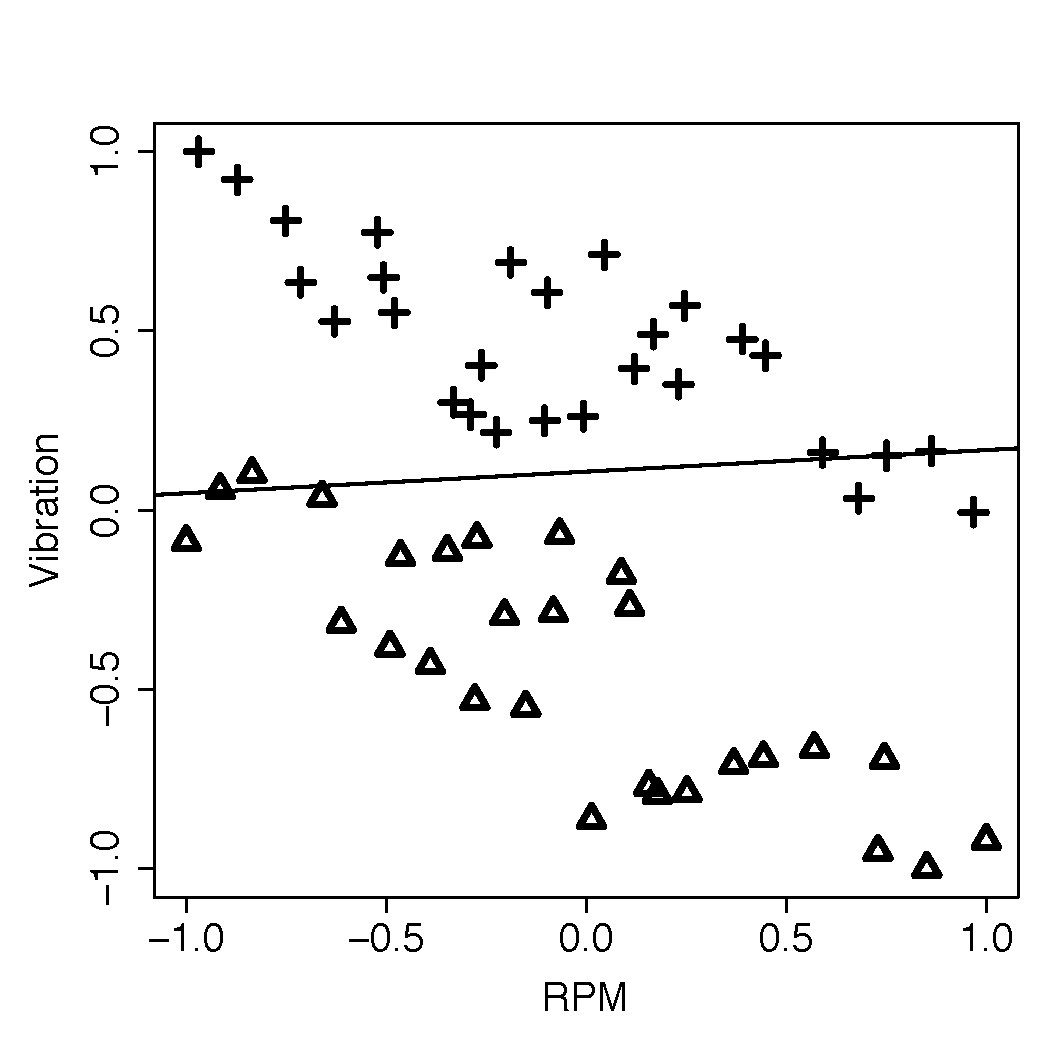
\includegraphics[width=0.27\textwidth]{./images/gradientDescentLogisticClassificationDemoGoodSep74.pdf}}
	\subfigure{\label{fig:machineryGoodSepGradientDescentSmallMultiples7}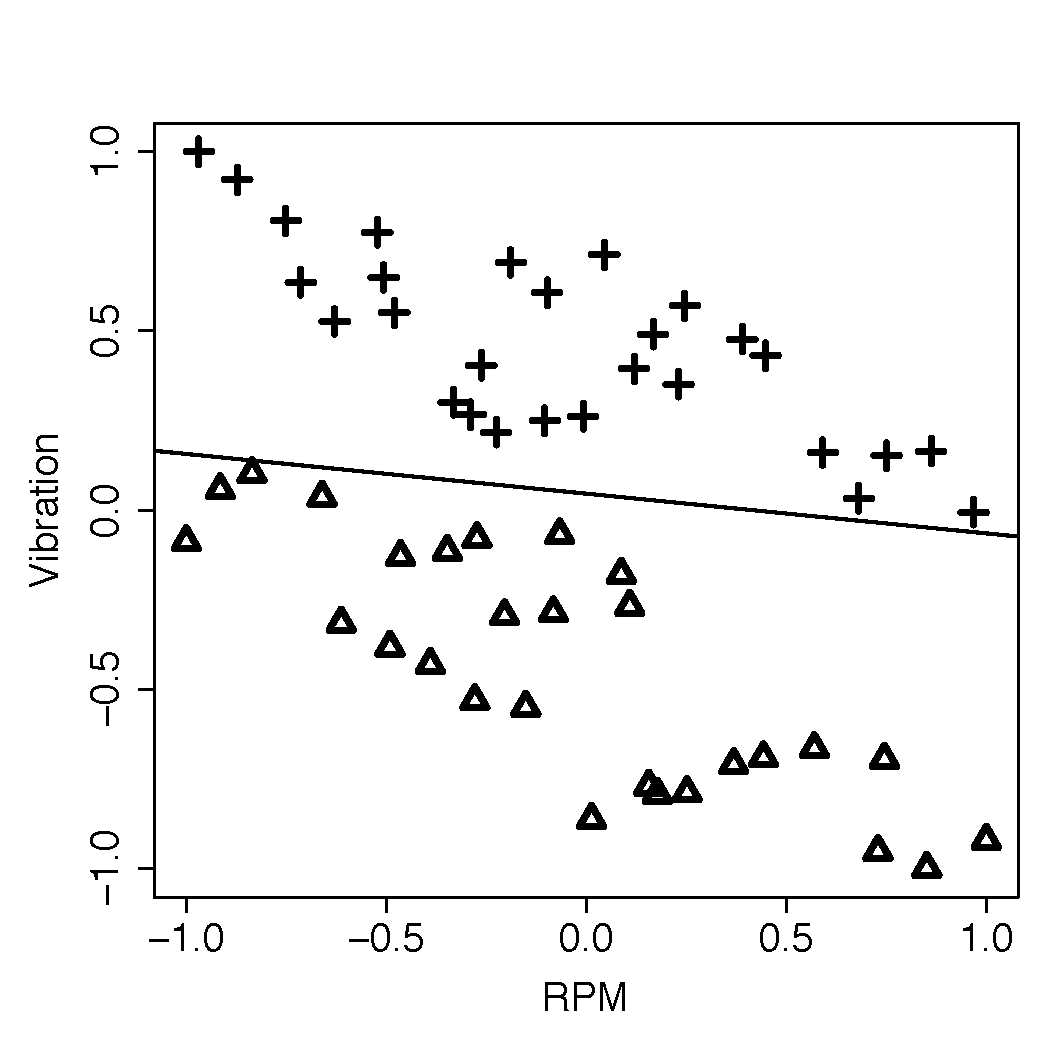
\includegraphics[width=0.27\textwidth]{./images/gradientDescentLogisticClassificationDemoGoodSep114.pdf}}
	\subfigure{\label{fig:machineryGoodSepGradientDescentSmallMultiples9}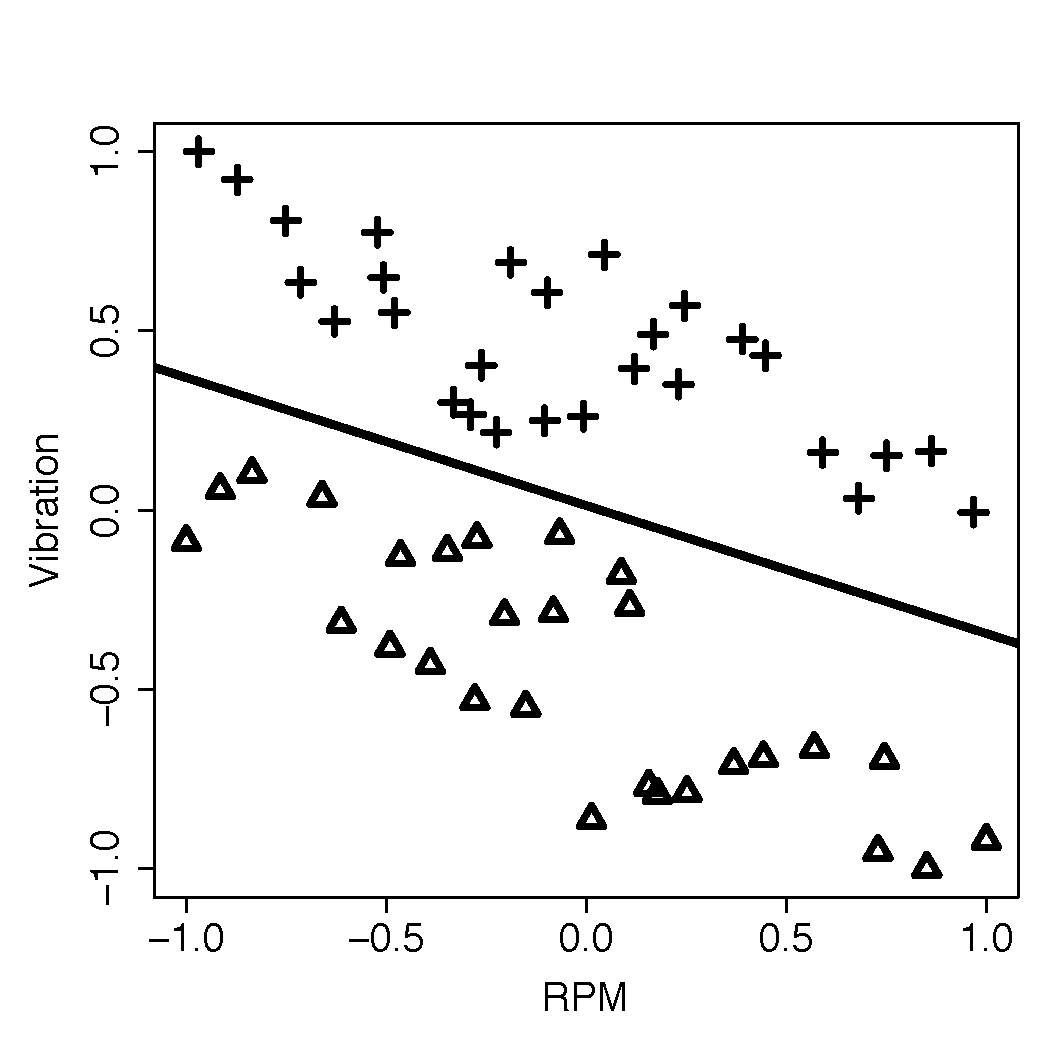
\includegraphics[width=0.27\textwidth]{./images/gradientDescentLogisticClassificationDemoGoodSepFinal.pdf}}
	\subfigure{\label{fig:machineryGoodSepGradientDescentSmallMultiplesJourney}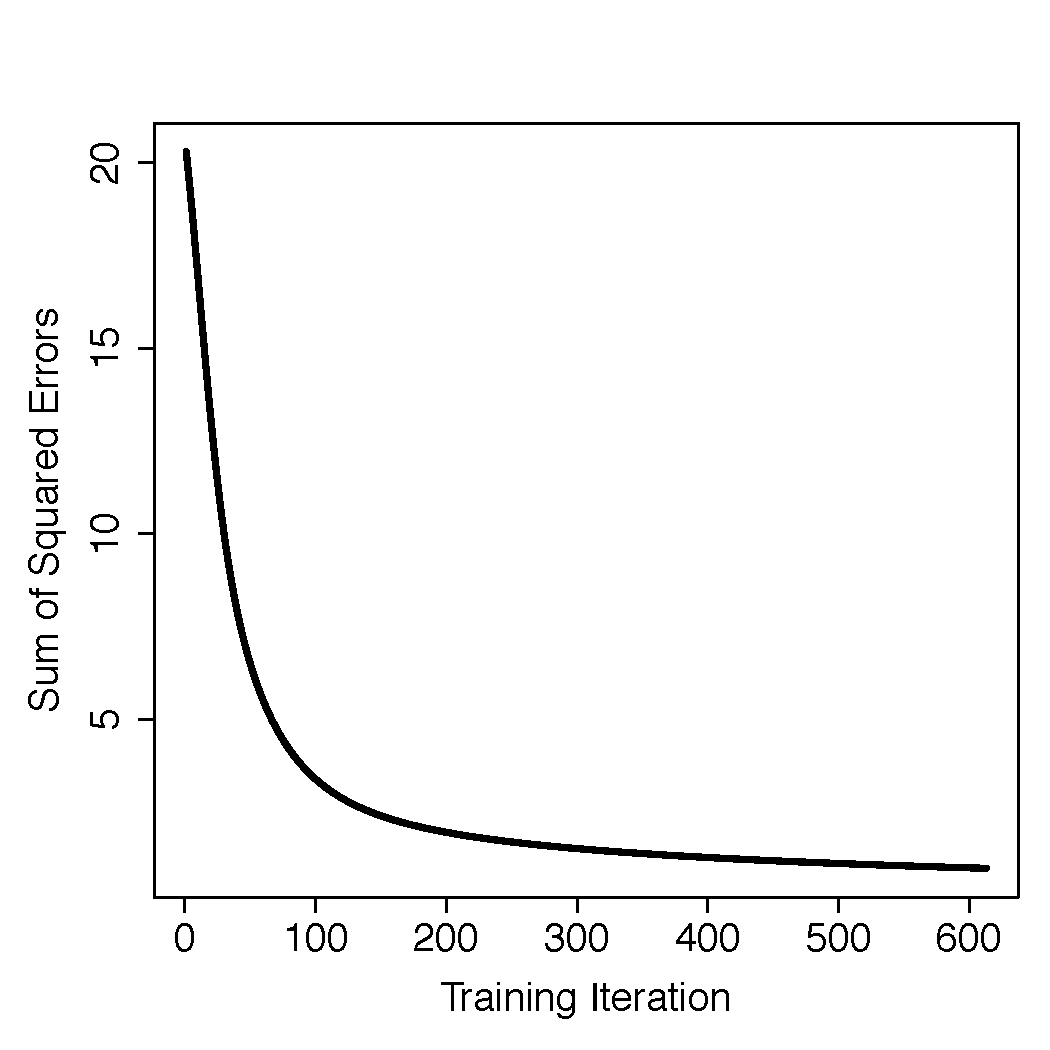
\includegraphics[width=0.27\textwidth]{./images/gradientDescentLogisticClassificationDemoGoodSepErrorJourney.pdf}}
\caption{A selection of the logistic regression models developed during the gradient descent process for the machinery dataset from Table \ourRef{tab:faultyMachineryData}. The bottom-right panel shows the sum of squared error values generated during the gradient descent process.}
\label{fig:machineryGoodSepGradientDescentSmallMultiples}
\end{center}
\end{figure}
\end{frame} 

\begin{frame} 
\begin{itemize}
\item To repurpose the gradient descent algorithm for training logistic regression models the only change that needs to be made is i in the weight update rule. 
\item See pg. 360 in book for details of how to derive the new weight update rule.
\item The new weight update rule is:
\end{itemize}
\begin{alignat*}{1}
	\mathbf{w}[j] \leftarrow \mathbf{w}[j] + \alpha \times \sum_{i=1}^{n} \left(\left(t - \mathbb{M}_{\mathbf{w}}(\mathbf{d}_i)\right) \times  \mathbb{M}_{\mathbf{w}}(\mathbf{d}_i) \times (1 - \mathbb{M}_{\mathbf{w}}(\mathbf{d}_i)) \times \mathbf{d}_i[j]\right)
	\label{eqn:logisticWeightUpdateRule}
\end{alignat*}
\end{frame} 

 \begin{frame}[plain]
\begin{table}[!thb]
\label{tab:faultyMachineryDataNonLinSep}
\centering
\begin{tiny}
\resizebox{\textwidth}{!}{
\begin{tabular}{cc}
		\hline
			\begin{minipage}{0.48\textwidth}
					\begin{tabular}[ht]{ c c c c }
\featN{ID} & \featN{RPM} & \featN{Vibration} & \featN{Status} \\
		\hline
1	&	498	&	604	&	faulty	\\
2	&	517	&	594	&	faulty		\\
3	&	541	&	574	&	faulty	\\
4	&	555	&	587	&	faulty		\\
5	&	572	&	537	&	faulty	\\
6	&	600	&	553	&	faulty		\\
7	&	621	&	482	&	faulty		\\
8	&	632	&	539	&	faulty		\\
9	&	656	&	476	&	faulty		\\
10	&	653	&	554	&	faulty		\\
11	&	679	&	516	&	faulty		\\
12	&	688	&	524	&	faulty		\\
13	&	684	&	450	&	faulty		\\
14	&	699	&	512	&	faulty		\\
15	&	703	&	505	&	faulty		\\
16	&	717	&	377	&	faulty	\\
17	&	740	&	377	&	faulty	\\
18	&	749	&	501	&	faulty	\\
19	&	756	&	492	&	faulty	\\
20	&	752	&	381	&	faulty		\\
21	&	762	&	508	&	faulty	\\
22	&	781	&	474	&	faulty	\\
23	&	781	&	480	&	faulty	\\
24	&	804	&	460	&	faulty	\\
25	&	828	&	346	&	faulty	\\
26	&	830	&	366	&	faulty	\\
27	&	864	&	344	&	faulty		\\
28	&	882	&	403	&	faulty	\\
29	&	891	&	338	&	faulty	\\
30	&	921	&	362	&	faulty		\\
31	&	941	&	301	&	faulty	\\
32	&	965	&	336	&	faulty		\\
33	&	976	&	297	&	faulty	\\
34	&	994	&	287	&	faulty		\\
		\hline
					\end{tabular}
			\end{minipage}
			&
			\begin{minipage}{0.48\textwidth}
										\begin{tabular}[ht]{ c c c c }
\featN{ID} & \featN{RPM} & \featN{Vibration} & \featN{Status} \\
		\hline
35	&	501	&	463	&	good	\\
36	&	526	&	443	&	good	\\
37	&	536	&	412	&	good	\\
38	&	564	&	394	&	good	\\
39	&	584	&	398	&	good	\\
40	&	602	&	398	&	good	\\
41	&	610	&	428	&	good	\\
42	&	638	&	389	&	good	\\
43	&	652	&	394	&	good	\\
44	&	659	&	336	&	good	\\
45	&	662	&	364	&	good	\\
46	&	672	&	308	&	good	\\
47	&	691	&	248	&	good	\\
48	&	694	&	401	&	good	\\
49	&	718	&	313	&	good	\\
50	&	720	&	410	&	good	\\
51	&	723	&	389	&	good	\\
52	&	744	&	227	&	good	\\
53	&	741	&	397	&	good	\\
54	&	770	&	200	&	good	\\
55	&	764	&	370	&	good	\\
56	&	790	&	248	&	good	\\
57	&	786	&	344	&	good	\\
58	&	792	&	290	&	good	\\
59	&	818	&	268	&	good	\\
60	&	845	&	232	&	good	\\
61	&	867	&	195	&	good	\\
62	&	878	&	168	&	good	\\
63	&	895	&	218	&	good	\\
64	&	916	&	221	&	good	\\
65	&	950	&	156	&	good	\\
66	&	956	&	174	&	good	\\
67	&	973	&	134	&	good	\\
68	&	1002	&	121	&	good	\\
\hline
				\end{tabular}
			\end{minipage}\\
\end{tabular}
}
\end{tiny}
\end{table}
\end{frame} 



 \begin{frame} [plain]
\begin{figure}[htb]
\begin{center}
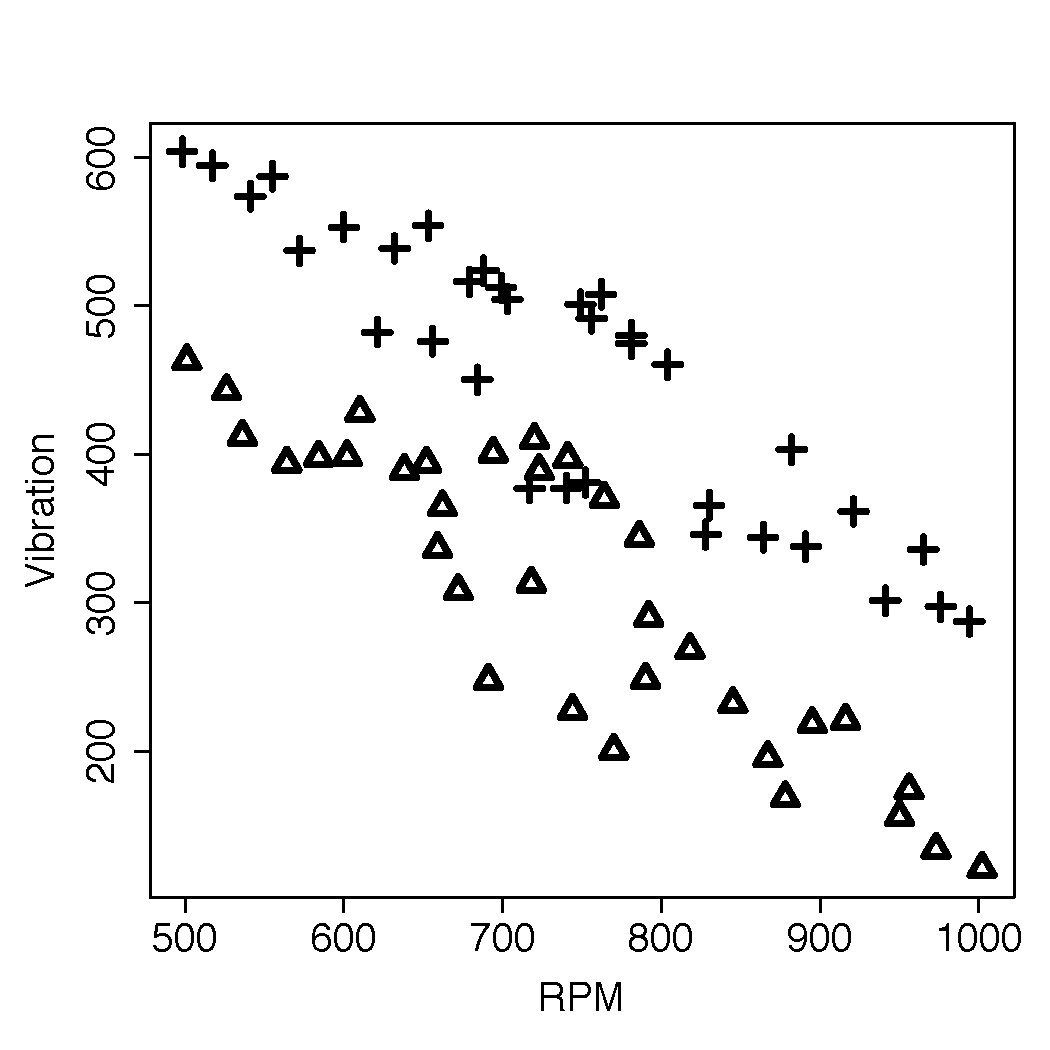
\includegraphics[width=0.65\textwidth]{./images/gradientDescentLogisticClassificationDemoBadSepDataset.pdf}
	\caption{A scatter plot of the extended generators dataset given in Table \ourRef{tab:faultyMachineryDataNonLinSep}, which results in instances with the different target levels overlapping with each other. \featL{good} generators are shown as crosses, and \featL{faulty} generators are shown as triangles.}
	\label{fig:faultyMachinesDataNonLinearSep}
\end{center}
\end{figure}
\end{frame} 

\begin{frame}
\begin{itemize}
	\item For logistic regression models we recommend that descriptive feature values always be normalized. 
	\item In this example, before the training process begins, both descriptive features are normalized to the range $\left[-1, 1\right]$.
\end{itemize}
\end{frame}


 \begin{frame} 
 \begin{itemize}
\item For this example let's assume that:
	\begin{itemize}
		\item $\alpha = 0.02$ 
	\end{itemize}
\end{itemize}
	\begin{footnotesize}
	\begin{center}
	\begin{tabular}{c c c c c c}
			\multicolumn{6}{c}{\textbf{Initial Weights}} \\
			\hline
			$\mathbf{w}[0]$: &	-2.9465	& 	$\mathbf{w}[1]$:	&	-1.0147	 & $\mathbf{w}[2]$: &	-2.1610 \\
			\hline
	\end{tabular}
	\end{center}
	\end{footnotesize}
\end{frame}
	
\begin{frame}
\begin{footnotesize}
\resizebox{\linewidth}{!}{
	\begin{tabular}{ c c c c c | c c c }
		\multicolumn{8}{ c }{\textbf{Iteration 1}}	\\
		\hline
				~ & \featN{Target} & ~ & ~ & Squared & \multicolumn{3}{c}{$\mathbf{errorDelta(\mathcal{D}, w[i])}$} \\
		\featN{ID} & \featN{Level} & Pred. & Error & Error & $\mathbf{w}[0]$ & $\mathbf{w}[1]$ & $\mathbf{w}[2]$ \\
		\hline
1	&	1	&	0.5570	&	0.4430	&	0.1963	&	0.1093	&	-0.1093	&	0.1093	\\
2	&	1	&	0.5168	&	0.4832	&	0.2335	&	0.1207	&	-0.1116	&	0.1159	\\
3	&	1	&	0.4469	&	0.5531	&	0.3059	&	0.1367	&	-0.1134	&	0.1197	\\
4	&	1	&	0.4629	&	0.5371	&	0.2885	&	0.1335	&	-0.1033	&	0.1244	\\
		\multicolumn{8}{c}{$ \cdot  \cdot  \cdot $}	\\
65	&	0	&	0.0037	&	-0.0037	&	0.0000	&	0.0000	&	0.0000	&	0.0000	\\
66	&	0	&	0.0042	&	-0.0042	&	0.0000	&	0.0000	&	0.0000	&	0.0000	\\
67	&	0	&	0.0028	&	-0.0028	&	0.0000	&	0.0000	&	0.0000	&	0.0000	\\
68	&	0	&	0.0022	&	-0.0022	&	0.0000	&	0.0000	&	0.0000	&	0.0000	\\
		\hline									
		\multicolumn{4}{r}{\textbf{Sum }} & 24.4738	&	2.7031	&	-0.7015	&	1.6493	\\
		\multicolumn{4}{r}{\textbf{Sum of squared errors ($\mathbf{Sum/2}$)}} & 12.2369 &  & & \\
		\hline
		\end{tabular}
		}%end resize box
	\end{footnotesize}
\end{frame}


\begin{frame}
\begin{equation*}
	\mathbf{w}[j] \leftarrow \mathbf{w}[j] + \alpha \times \sum_{i=1}^{n} \left(\left(t_i - \mathbb{M}_{\mathbf{w}}(\mathbf{d}_i)\right) \times  \mathbb{M}_{\mathbf{w}}(\mathbf{d}_i) \times (1 - \mathbb{M}_{\mathbf{w}}(\mathbf{d}_i)) \times \mathbf{d}_i[j]\right)
\end{equation*}
\begin{center}
\begin{footnotesize}
\begin{tabular}{c c c c c c}
			\multicolumn{6}{c}{\textbf{New Weights (after Iteration 1)}} \\
			\hline
			$\mathbf{w}[0]$: &	-2.8924	& 	$\mathbf{w}[1]$:	&	-1.0287	 & $\mathbf{w}[2]$: &	-2.1940 \\
			\hline
	\end{tabular}
\end{footnotesize}
\end{center}
\end{frame}
	
\begin{frame}
	\begin{footnotesize}	
	\resizebox{\linewidth}{!}{
	\begin{tabular}{ c c c c c | c c c }
		\multicolumn{8}{ c }{\textbf{Iteration 2}}	\\
		\hline
				~ & \featN{Target} & ~ & \textbf{} & Squared & \multicolumn{3}{c}{$\mathbf{errorDelta(\mathcal{D}, w[i])}$} \\
		\featN{ID} & \featN{Level} & Pred. & Error & Error & $\mathbf{w}[0]$ & $\mathbf{w}[1]$ & $\mathbf{w}[2]$ \\
		\hline	
1	&	1	&	0.5817	&	0.4183	&	0.1749	&	0.1018	&	-0.1018	&	0.1018	\\
2	&	1	&	0.5414	&	0.4586	&	0.2103	&	0.1139	&	-0.1053	&	0.1094	\\
3	&	1	&	0.4704	&	0.5296	&	0.2805	&	0.1319	&	-0.1094	&	0.1155	\\
4	&	1	&	0.4867	&	0.5133	&	0.2635	&	0.1282	&	-0.0992	&	0.1194	\\
		\multicolumn{8}{c}{$ \cdot  \cdot  \cdot $}	\\
65	&	0	&	0.0037	&	-0.0037	&	0.0000	&	0.0000	&	0.0000	&	0.0000	\\
66	&	0	&	0.0043	&	-0.0043	&	0.0000	&	0.0000	&	0.0000	&	0.0000	\\
67	&	0	&	0.0028	&	-0.0028	&	0.0000	&	0.0000	&	0.0000	&	0.0000	\\
68	&	0	&	0.0022	&	-0.0022	&	0.0000	&	0.0000	&	0.0000	&	0.0000	\\						
		\hline
	\multicolumn{4}{r}{\textbf{Sum }} & 24.0524	&	2.7236	&	-0.6646	&	1.6484	\\
		\multicolumn{4}{r}{\textbf{Sum of squared errors ($\mathbf{Sum/2}$)}} & 12.0262 &  & &  \\
		\hline
	\end{tabular}
	}%end resizebox
	\end{footnotesize}
\end{frame}

\begin{frame}
\begin{equation*}
	\mathbf{w}[j] \leftarrow \mathbf{w}[j] + \alpha \times \sum_{i=1}^{n} \left(\left(t_i - \mathbb{M}_{\mathbf{w}}(\mathbf{d}_i)\right) \times  \mathbb{M}_{\mathbf{w}}(\mathbf{d}_i) \times (1 - \mathbb{M}_{\mathbf{w}}(\mathbf{d}_i)) \times \mathbf{d}_i[j]\right)
\end{equation*}
\begin{center}
\begin{footnotesize}
\begin{tabular}{c c c c c c}
			\multicolumn{6}{c}{\textbf{New Weights (after Iteration 2)}} \\
			\hline
			$\mathbf{w}[0]$: &	-2.8380	& 	$\mathbf{w}[1]$:	&	-1.0416	 & $\mathbf{w}[2]$: &	-2.2271 \\
			\hline
	\end{tabular}
\end{footnotesize}
\end{center}
\end{frame}

\begin{frame} [plain]
\begin{footnotesize}
\begin{figure}[htb]
\begin{center}
	\subfigure{\label{fig:machineryBadSepGradientDescentSmallMultiples1}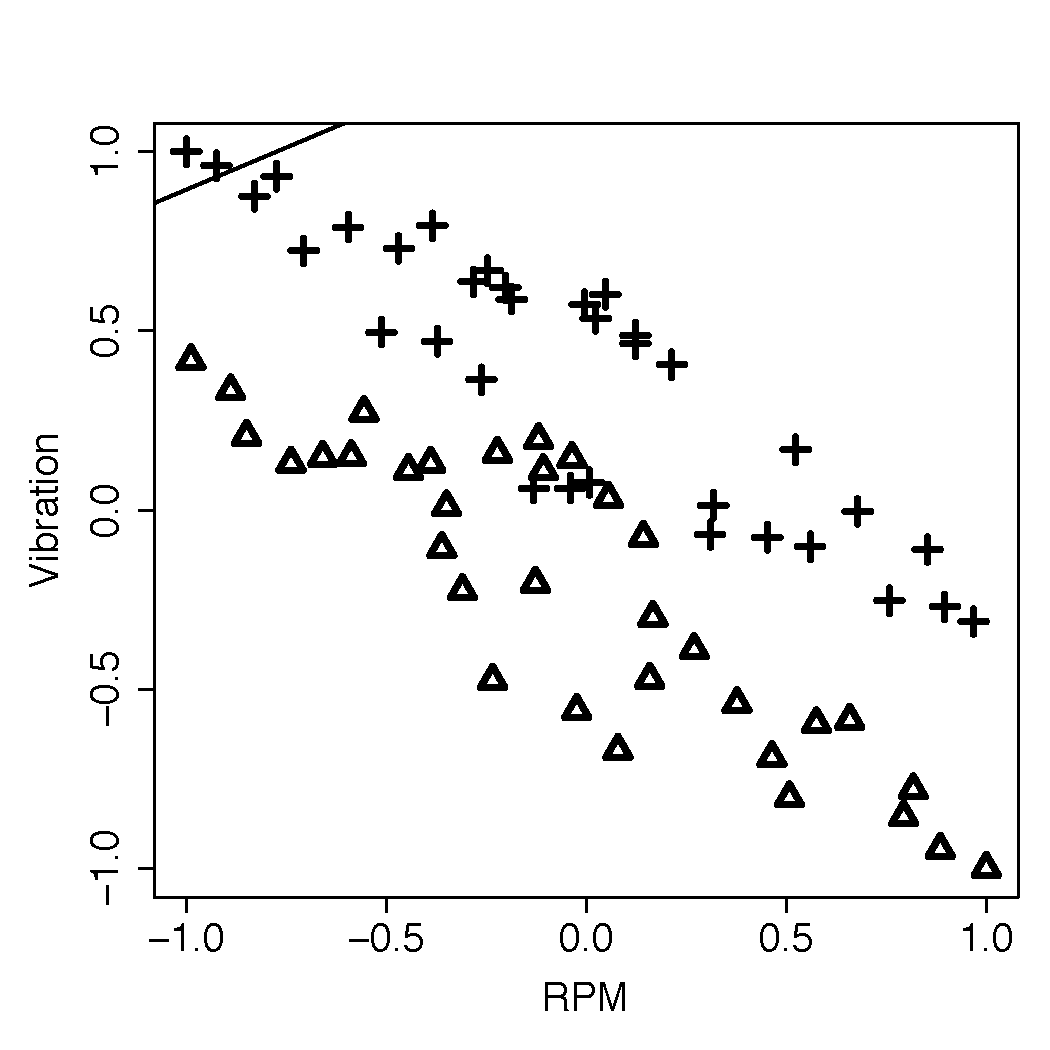
\includegraphics[width=0.27\textwidth]{./images/gradientDescentLogisticClassificationDemoBadSep0.pdf}}
	\subfigure{\label{fig:machineryBadSepGradientDescentSmallMultiples3}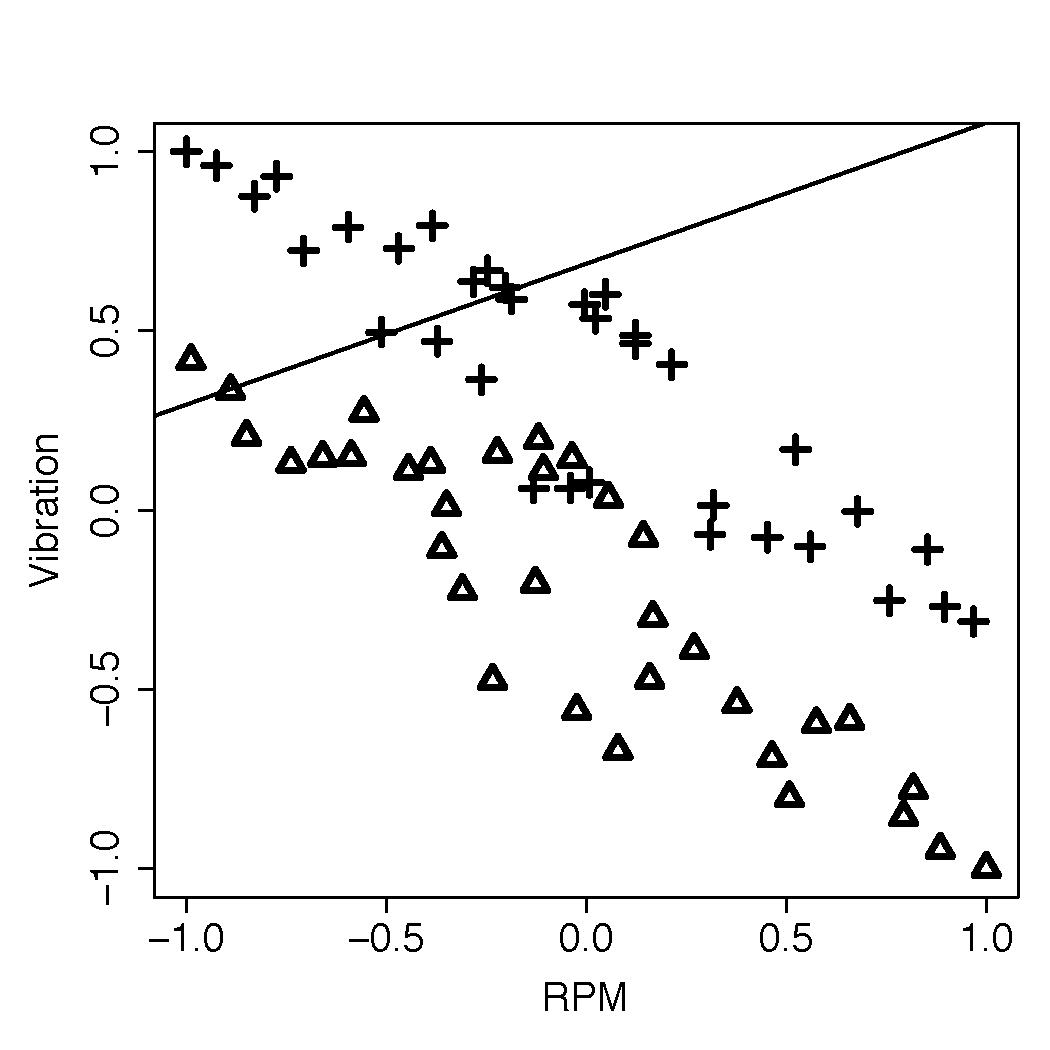
\includegraphics[width=0.27\textwidth]{./images/gradientDescentLogisticClassificationDemoBadSep21.pdf}}
	\subfigure{\label{fig:machineryBadSepGradientDescentSmallMultiples5}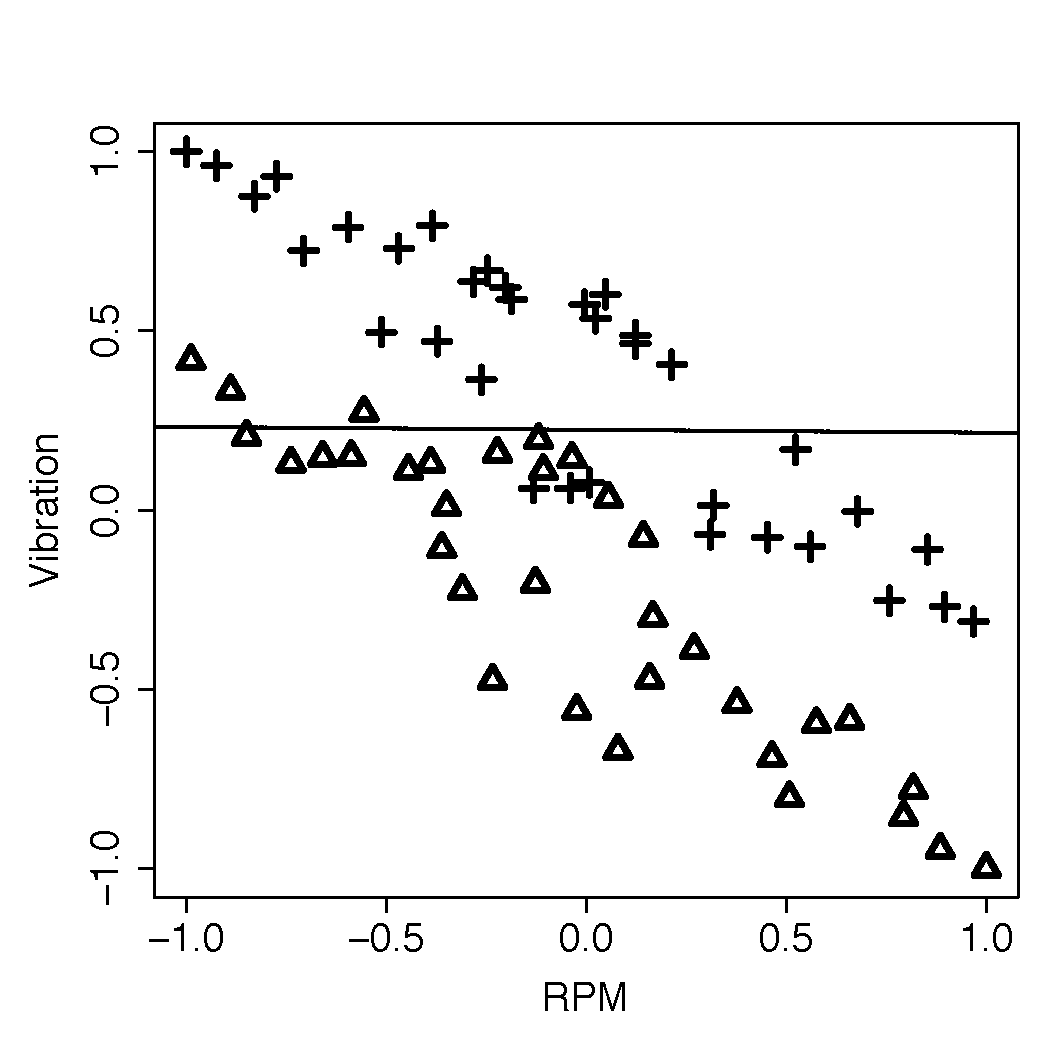
\includegraphics[width=0.27\textwidth]{./images/gradientDescentLogisticClassificationDemoBadSep71.pdf}}	
	\subfigure{\label{fig:machineryBadSepGradientDescentSmallMultiples7}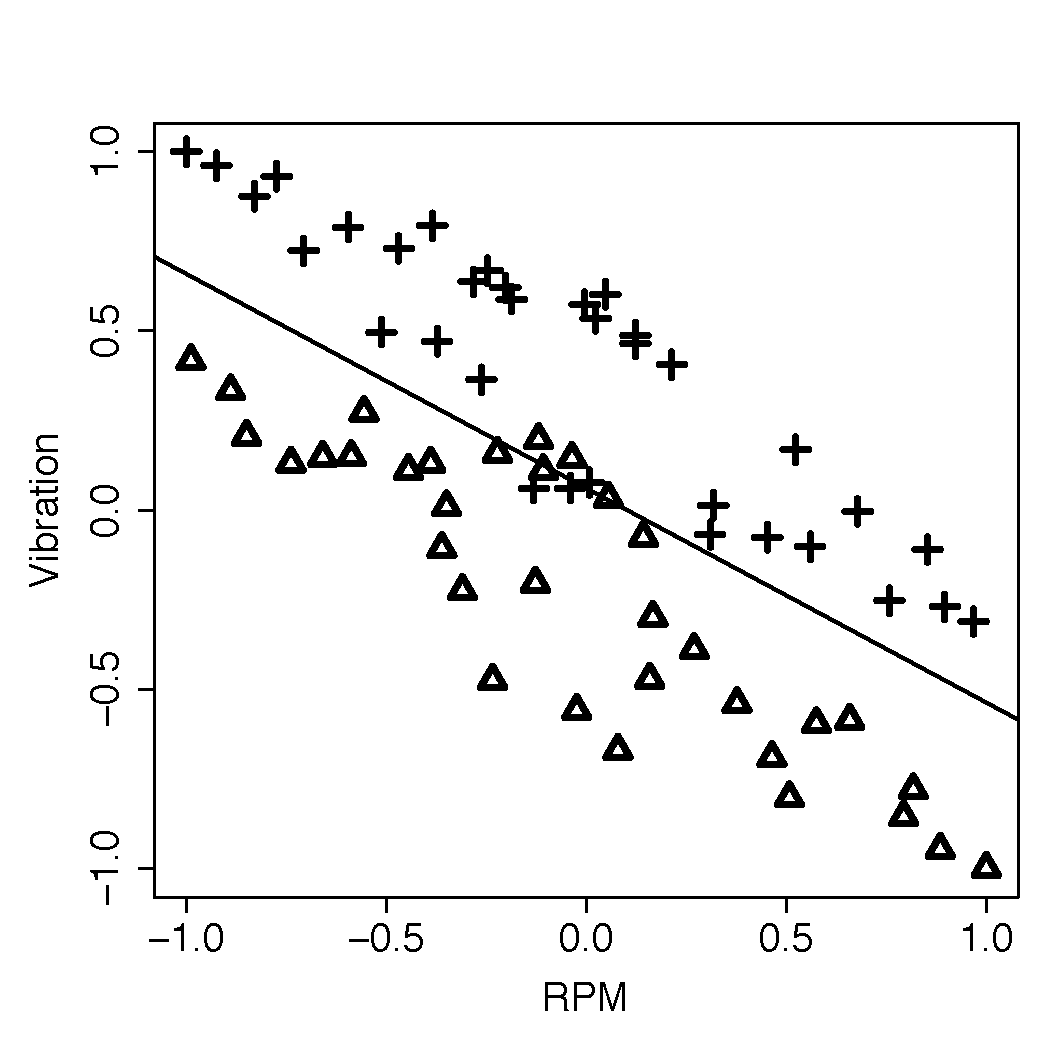
\includegraphics[width=0.27\textwidth]{./images/gradientDescentLogisticClassificationDemoBadSep233.pdf}}
	\subfigure{\label{fig:machineryBadSepGradientDescentSmallMultiples9}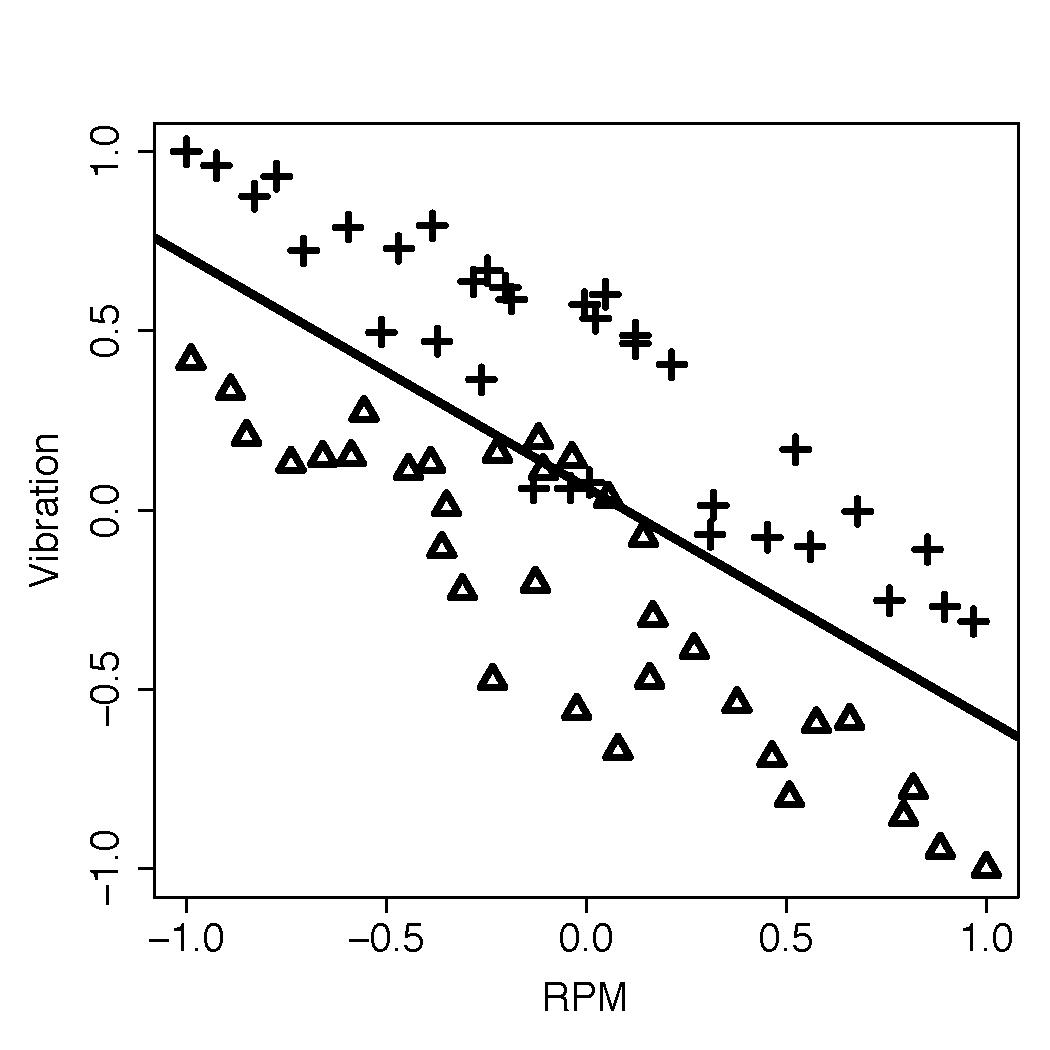
\includegraphics[width=0.27\textwidth]{./images/gradientDescentLogisticClassificationDemoBadSepFinal.pdf}}
	\subfigure{\label{fig:machineryBadSepGradientDescentSmallMultiplesJourney}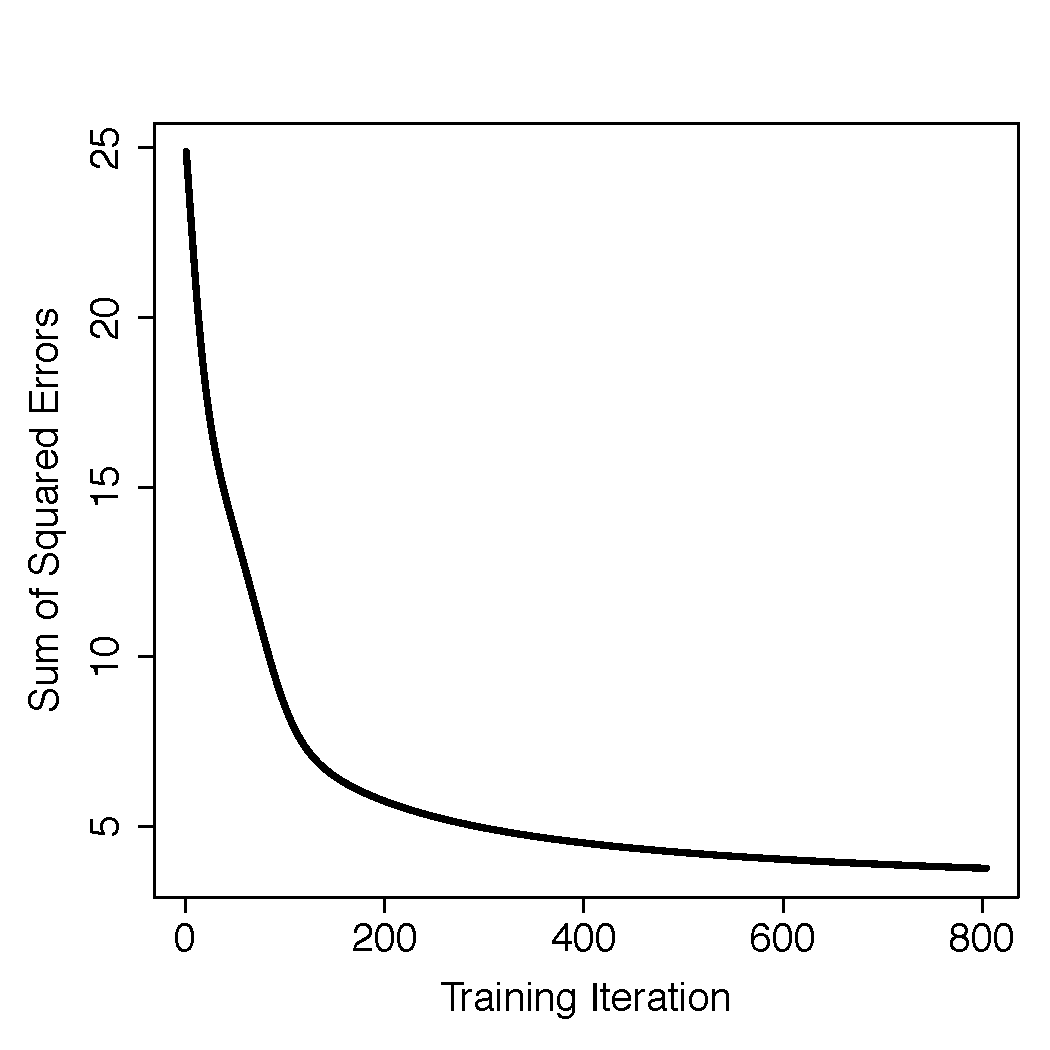
\includegraphics[width=0.27\textwidth]{./images/gradientDescentLogisticClassificationDemoBadSepErrorJourney.pdf}}
\caption{A selection of the logistic regression models developed during the gradient descent process for the extended generators dataset in Table \ourRef{tab:faultyMachineryDataNonLinSep}. The bottom-right panel shows the sum of squared error values generated during the gradient descent process.}
\label{fig:machineryBadSepGradientDescentSmallMultiples}
\end{center}
\end{figure}
\end{footnotesize}
\end{frame} 

 \begin{frame} 
 \begin{itemize}
 \item The final model found is:
 \end{itemize}
  
\begin{alignat*}{2}
		\mathbb{M}_{\mathbf{w}}(&\left< \featN{RPM},  \featN{Vibration} \right>) \\
		& = \frac{1}{1+e^{-(-0.4077 + 4.1697 \times \featN{RPM} + 6.0460 \times \featN{Vibration} )}}
		\label{eqn:faultyMachineryLogisticExample}
\end{alignat*}
\end{frame} 

\SectionSlideShortHeader{Modeling Non-linear Relationships}{Non-Linear Relationships}

 \begin{frame} 
\begin{table}[htb]
\caption{A dataset describing grass growth on Irish farms during July 2012.}
\label{tab:grassGrowthDataset}
\centering
\begin{scriptsize}
\begin{tabular}{ccc}
		\hline
			\noindent\begin{minipage}{0.3\textwidth}
					\begin{tabular}[ht]{ c c c }
		\featN{ID} & \featN{Rain} & \featN{Growth} \\
		\hline
1	&	2.153	&	14.016	\\
2	&	3.933	&	10.834	\\
3	&	1.699	&	13.026	\\
4	&	1.164	&	11.019	\\
5	&	4.793	&	4.162	\\
6	&	2.690	&	14.167	\\
7	&	3.982	&	10.190	\\
8	&	3.333	&	13.525	\\
9	&	1.942	&	13.899	\\
10	&	2.876	&	13.949	\\
11	&	4.277	&	8.643	\\
		\hline
					\end{tabular}
			\end{minipage}
			&
			\begin{minipage}{0.3\textwidth}
					\begin{tabular}[ht]{ c c c }
		\featN{ID} & \featN{Rain} & \featN{Growth} \\
		\hline
12	&	3.754	&	11.420	\\
13	&	2.809	&	13.847	\\
14	&	1.809	&	13.757	\\
15	&	4.114	&	9.101	\\
16	&	2.834	&	13.923	\\
17	&	3.872	&	10.795	\\
18	&	2.174	&	14.307	\\
19	&	4.353	&	8.059	\\
20	&	3.684	&	12.041	\\
21	&	2.140	&	14.641	\\
22	&	2.783	&	14.138	\\
\hline
				\end{tabular}
			\end{minipage}
			&
			\begin{minipage}{0.3\textwidth}
					\begin{tabular}[ht]{ c c c }
		\featN{ID} & \featN{Rain} & \featN{Growth} \\
		\hline
23	&	3.960	&	10.307	\\
24	&	3.592	&	12.069	\\
25	&	3.451	&	12.335	\\
26	&	1.197	&	10.806	\\
27	&	0.723	&	7.822	\\
28	&	1.958	&	14.010	\\
29	&	2.366	&	14.088	\\
30	&	1.530	&	12.701	\\
31	&	0.847	&	9.012	\\
32	&	3.843	&	10.885	\\
33	&	0.976	&	9.876	\\	
\hline
				\end{tabular}
			\end{minipage}\\
\end{tabular}
\end{scriptsize}
\end{table}
\end{frame} 

 \begin{frame}[plain]
\begin{figure}
\begin{center}
\label{fig:grassGrowthPlot}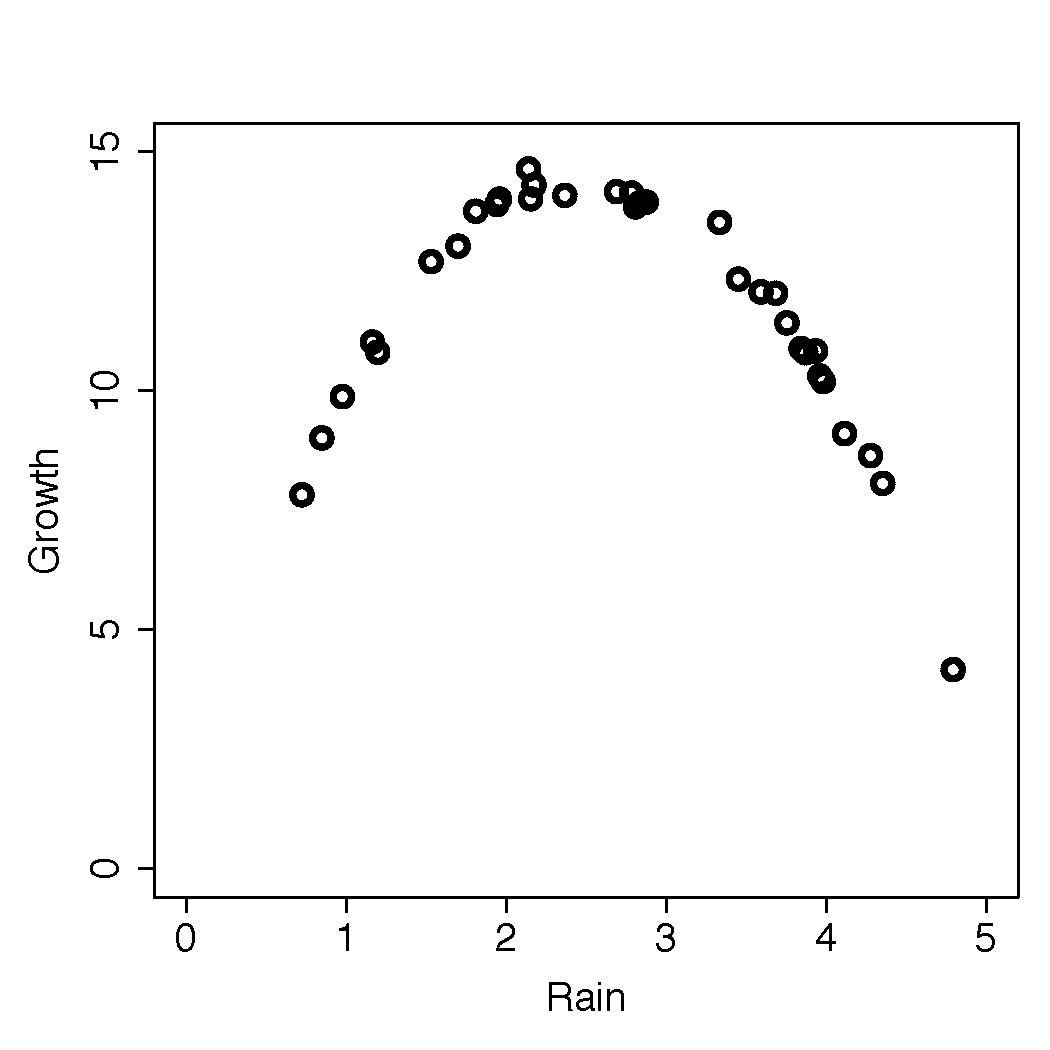
\includegraphics[width=0.75\textwidth]{./images/grassGrowthDataset.pdf}
\caption{A scatter plot of the \featN{Rain} and \featN{Growth} feature from the grass growth dataset.}
\label{fig:grassGrowth}
\end{center}
\end{figure}
\end{frame} 

 \begin{frame} 
 \begin{itemize}
 \item The best linear model we can learn for this data is: 
\begin{eqnarray*}
	\featN{Growth} = 13.510 + -0.667 \times \featN{Rain}
\end{eqnarray*}
 \end{itemize}
\begin{figure}
\begin{center}
\label{fig:grassGrowthLinearModel}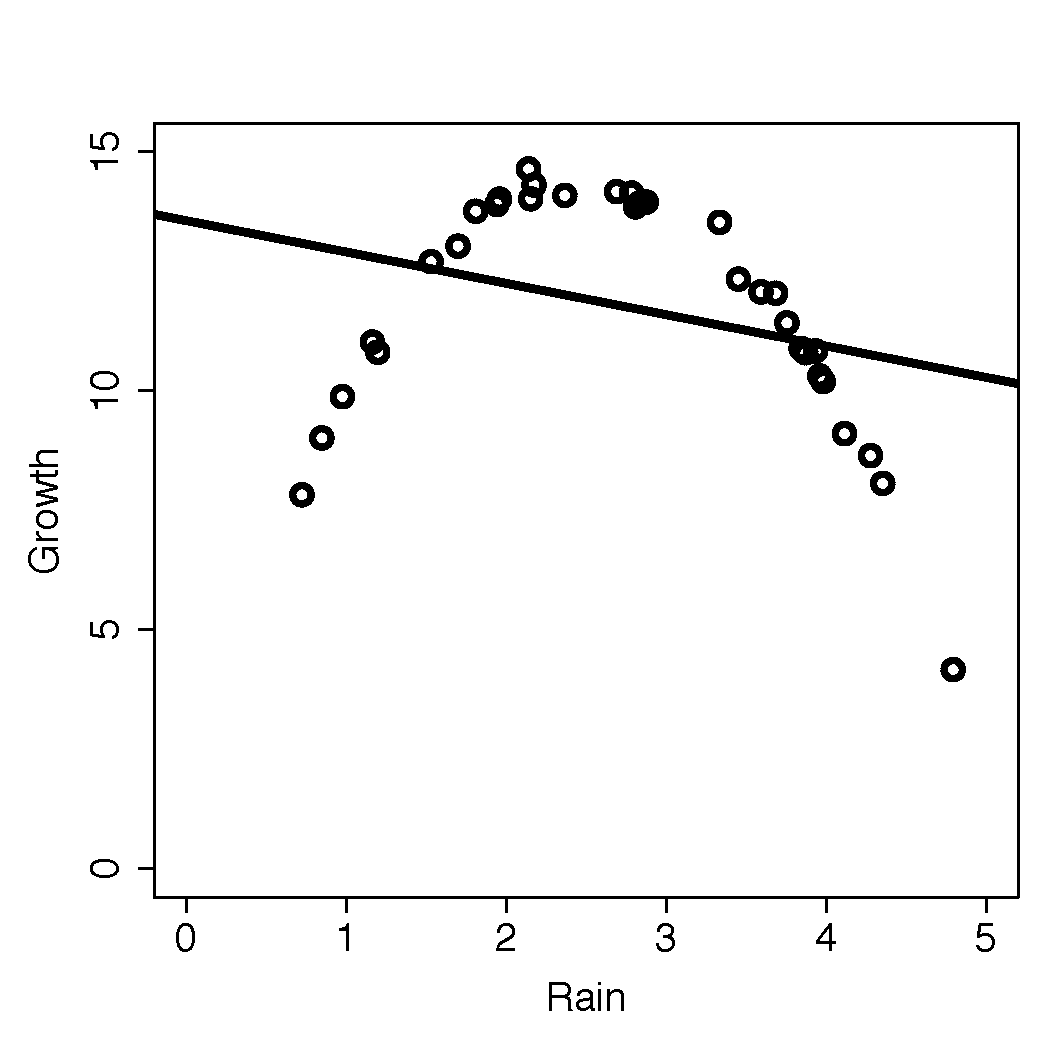
\includegraphics[width=0.45\textwidth]{./images/grassGrowthLinearModel.pdf}
\caption{A simple linear regression model trained to capture the relationship between the grass growth and rainfall.}
\label{fig:grassGrowth}
\end{center}
\end{figure}
\end{frame} 

\begin{frame}
\begin{itemize}
	\item In order to handle non-linear relationships we transform the data rather than the model using a set of basis functions:
\begin{eqnarray}
\mathbb{M}_{\mathbf{w}}(\mathbf{d}) & = & \sum_{k=0}^{b} \mathbf{w}[k]\times\phi_k(\mathbf{d})
\label{eqn:multiVariateRegressionWithBasisFunctions}
\end{eqnarray}
\noindent where $\phi_0$ to $\phi_b$ are a series of $b$ basis functions that each transform the input vector $\mathbf{d}$ in a different way. 
\item The advantage of this is that, except for introducing the mechanism of basis functions, we do not need to make any other changes to the approach we have presented so far. 
\end{itemize}
\end{frame} 

 \begin{frame} 
\begin{itemize}
	\item The relationship between rainfall and grass growth in the grass growth dataset can be accurately represented as a \keyword{second order polynomial} through the following model:

\noindent\begin{footnotesize}
\begin{eqnarray*}
\featN{Growth} = \mathbf{w}[0] \times \phi_0(\featN{Rain})+ \mathbf{w}[1] \times \phi_1(\featN{Rain}) + \mathbf{w}[2] \times \phi_2(\featN{Rain})
\end{eqnarray*}

~\\

where

\begin{eqnarray*}
\phi_0(\featN{Rain}) & = & 1 \\
\phi_1(\featN{Rain}) & = & \featN{Rain} \\
\phi_2(\featN{Rain}) & = & \featN{Rain}^2 
\end{eqnarray*}
\end{footnotesize}
\end{itemize}
\end{frame} 



 \begin{frame}[plain]
\begin{figure}[htb]
\begin{center}
	\subfigure{\label{fig:basisFunctionDemo1_1}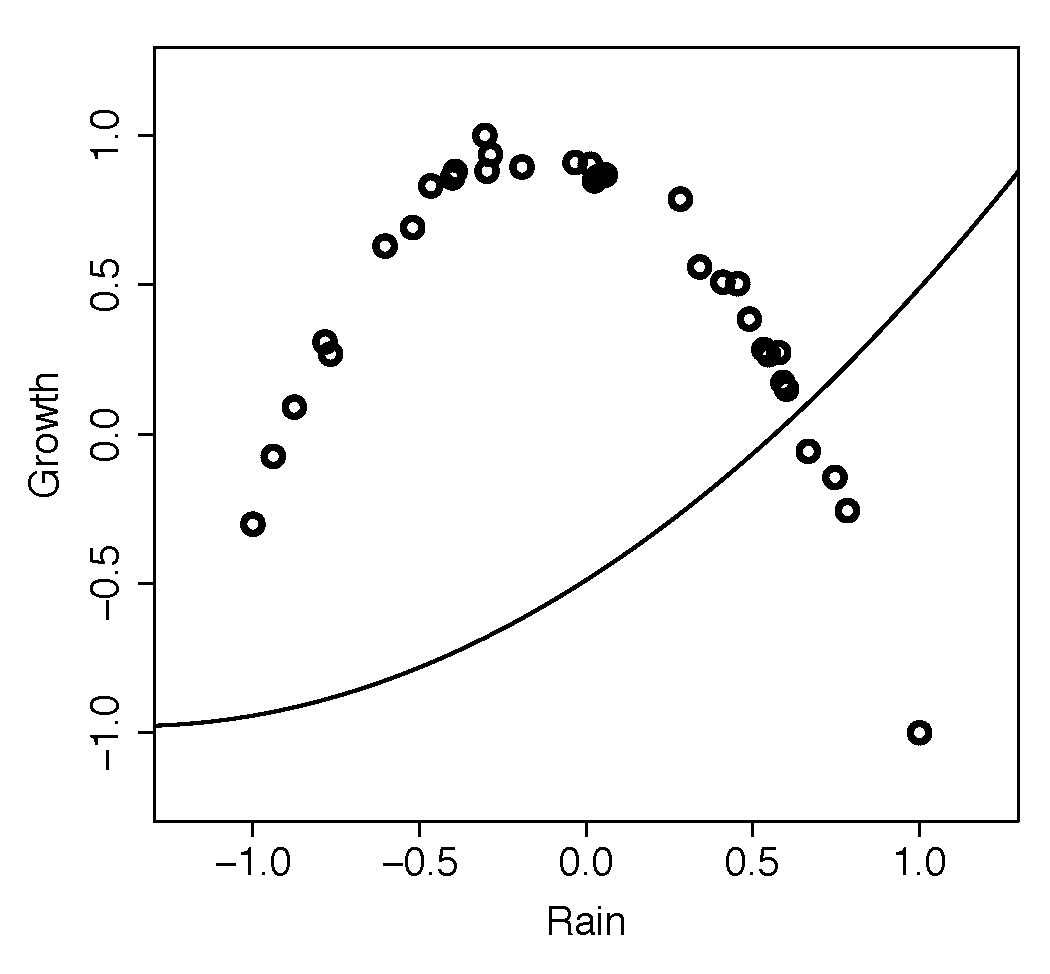
\includegraphics[width=0.27\textwidth]{./images/basisFunctionLinearRegressionDemo0.pdf}}
	\subfigure{\label{fig:basisFunctionDemo1_3}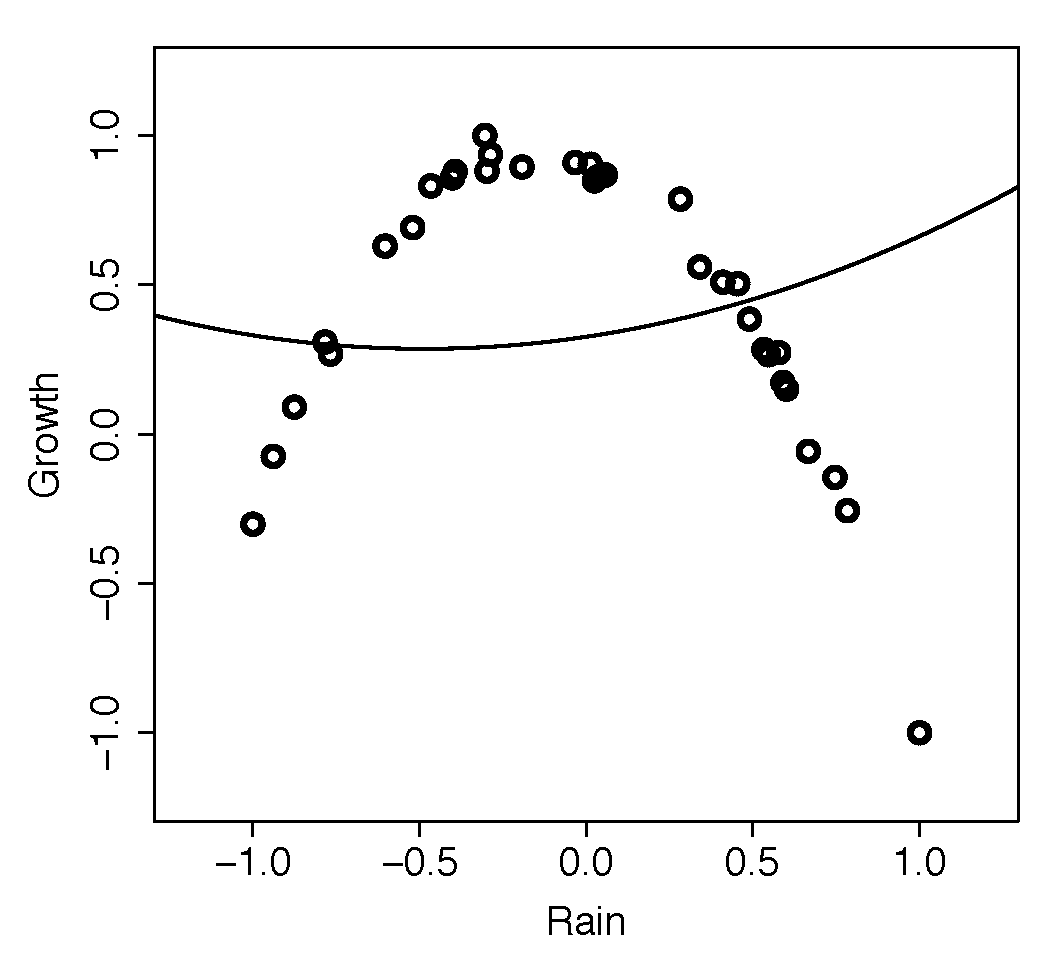
\includegraphics[width=0.27\textwidth]{./images/basisFunctionLinearRegressionDemo10.pdf}}
	\subfigure{\label{fig:basisFunctionDemo1_4}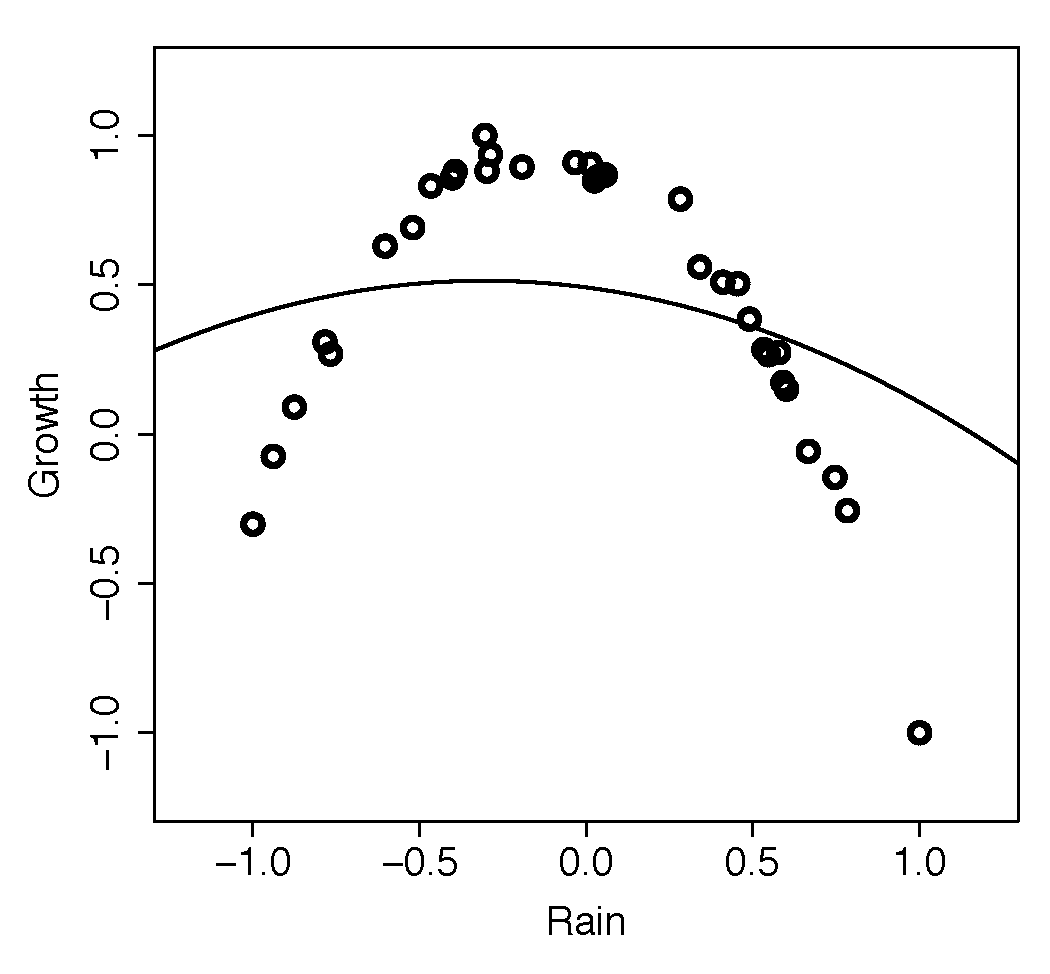
\includegraphics[width=0.27\textwidth]{./images/basisFunctionLinearRegressionDemo25.pdf}}
	\subfigure{\label{fig:basisFunctionDemo1_5}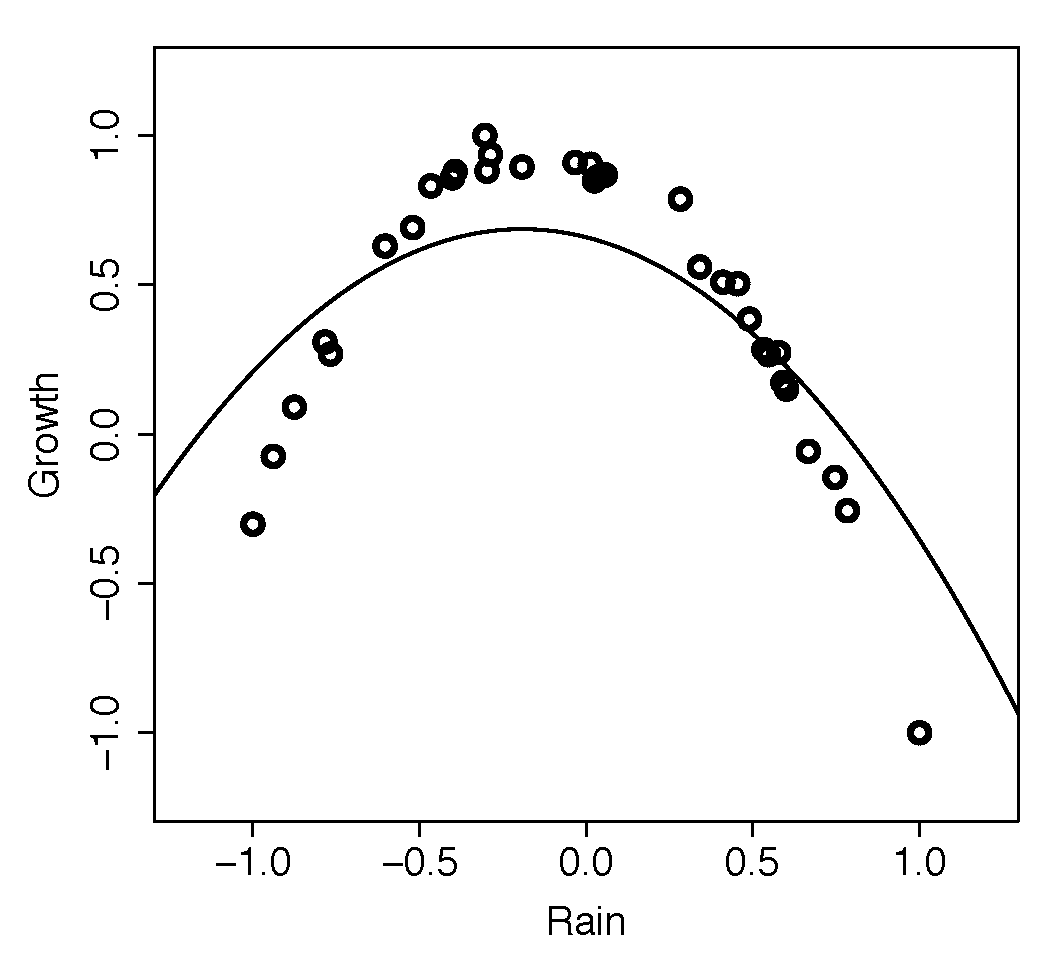
\includegraphics[width=0.27\textwidth]{./images/basisFunctionLinearRegressionDemo50.pdf}}
	\subfigure{\label{fig:basisFunctionDemo1_6}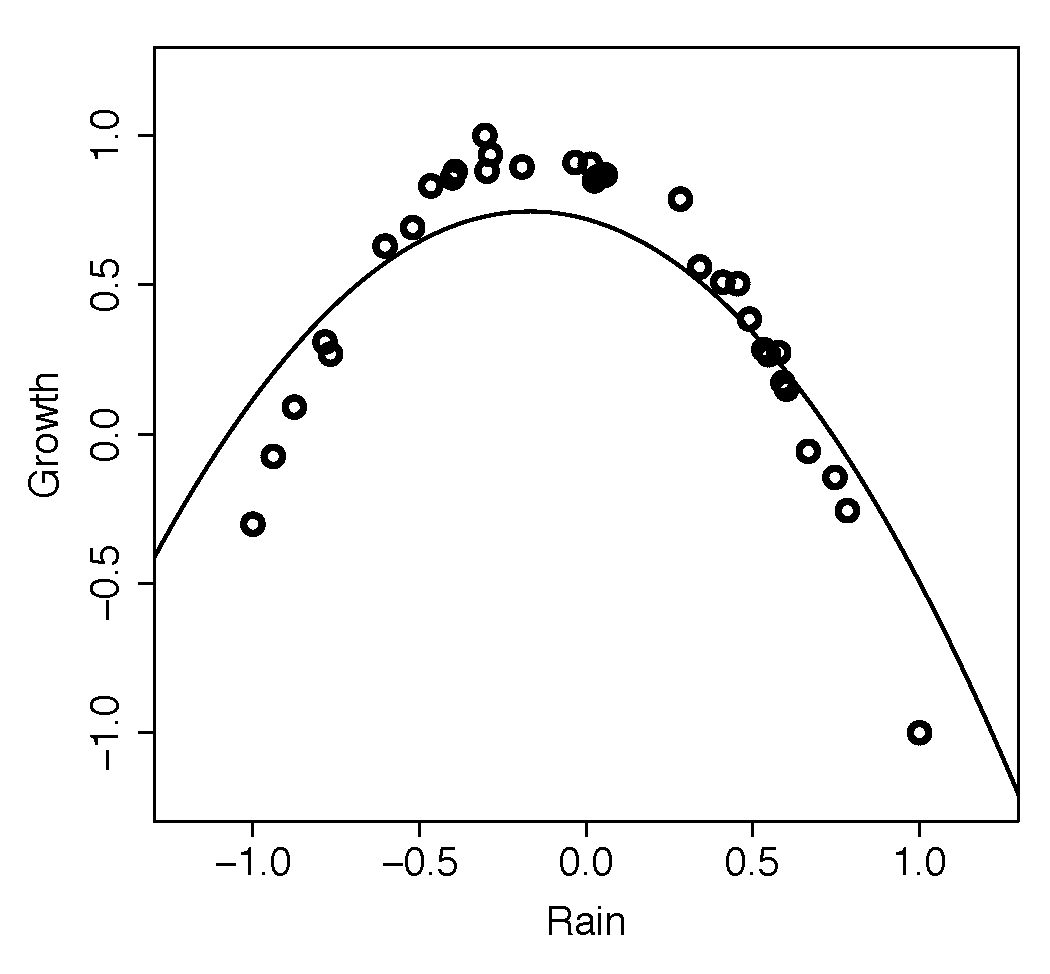
\includegraphics[width=0.27\textwidth]{./images/basisFunctionLinearRegressionDemo63.pdf}}
	\subfigure{\label{fig:basisFunctionDemo1_9}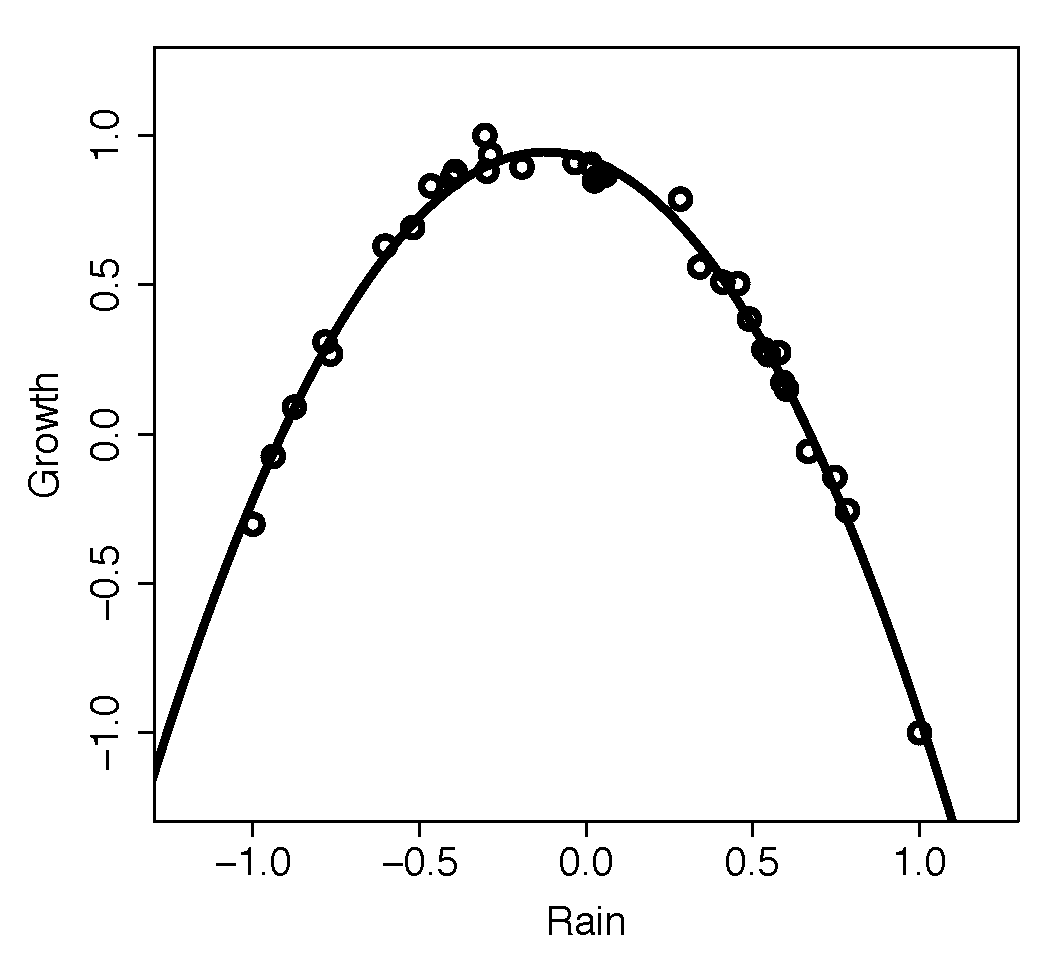
\includegraphics[width=0.27\textwidth]{./images/basisFunctionLinearRegressionDemoFinalModel.pdf}}
\caption{A selection of the models developed during the gradient descent process for the grass growth dataset from Table \ourRef{tab:grassGrowthDataset}. (Note that the \featN{Rain} and \featN{Growth} features have been \indexkeyword{range normalized} to the $[-1, 1]$ range.)}
\label{fig:basisFunctionDemo1}
\end{center}
\end{figure}
\end{frame} 


 \begin{frame}[plain]
 \begin{center}
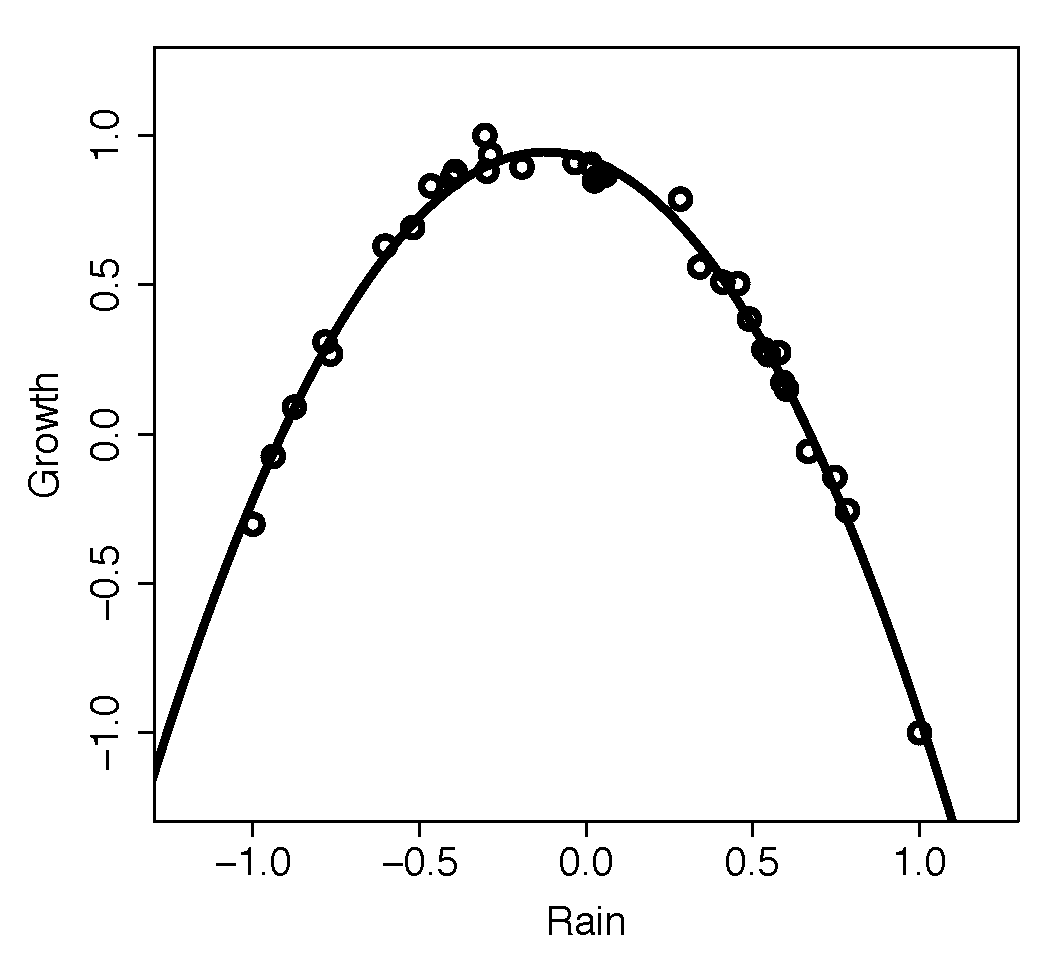
\includegraphics[width=0.65\textwidth]{./images/basisFunctionLinearRegressionDemoFinalModel.pdf}
\end{center}
\begin{footnotesize}
\begin{eqnarray*}
\featN{Growth} = 0.3707 \times \phi_0(\featN{Rain})+ 0.8475 \times \phi_1(\featN{Rain}) + -1.717 \times \phi_2(\featN{Rain})
\end{eqnarray*}
\end{footnotesize}
\end{frame} 


 \begin{frame}[plain]
\begin{footnotesize}
\begin{eqnarray*}
\featN{Growth} = 0.3707 \times \phi_0(\featN{Rain})+ 0.8475 \times \phi_1(\featN{Rain}) + -1.717 \times \phi_2(\featN{Rain})
\end{eqnarray*}
\end{footnotesize}
\begin{eqnarray*}
\phi_0(\featN{Rain}) & = & 1 \\
\phi_1(\featN{Rain}) & = & \featN{Rain} \\
\phi_2(\featN{Rain}) & = & \featN{Rain}^2 
\end{eqnarray*}
\begin{itemize}
	\item What is the predicted growth for the following \featN{Rain} values:
	\begin{enumerate}
		\item \featN{Rain}$=-0.75$
		\item \featN{Rain}$=0.1$
		\item \featN{Rain}$=0.9$
	\end{enumerate}
\end{itemize}
\end{frame} 


\begin{frame}
	\begin{itemize}
		\item Basis functions can also be used for 
		\begin{enumerate}
			\item multivariable simple linear regression models in the same way, the only extra requirement being the definition of more basis functions. 
			\item to train logistic regression models for categorical prediction problems that involve non-linear relationships.
		\end{enumerate}
	\end{itemize}
\end{frame}

 \begin{frame} 
\begin{table}[htb]
\caption{A dataset showing participants' responses to viewing \featL{positive} and \featL{negative} images measured on the EEG \featN{P20} and \featN{P45} potentials.}
\label{tab:eegDataset}
\centering
\begin{scriptsize}
\begin{tabular}{cc}
		\hline
			\begin{minipage}{0.42\textwidth}
					\begin{tabular}[ht]{ c c c c }
		\featN{ID} & \featN{P20} & \featN{P45} &  \featN{Type} \\		
		\hline
1	&	0.4497	&	0.4499	&	negative\\
2	&	0.8964	&	0.9006	&	negative\\
3	&	0.6952	&	0.3760	&	negative\\
4	&	0.1769	&	0.7050	&	negative\\
5	&	0.6904	&	0.4505	&	negative\\
6	&	0.7794	&	0.9190	&	negative\\
\multicolumn{4}{c}{$\vdots$}\\
		\hline
					\end{tabular}
			\end{minipage}
			&
			\begin{minipage}{0.42\textwidth}
										\begin{tabular}[ht]{ c c c c }
		\featN{ID} & \featN{P20} & \featN{P45} &  \featN{Type} \\		
		\hline
26	&	0.0656	&	0.2244	&	positive	\\
27	&	0.6336	&	0.2312	&	positive	\\
28	&	0.4453	&	0.4052	&	positive	\\
29	&	0.9998	&	0.8493	&	positive	\\
30	&	0.9027	&	0.6080	&	positive	\\
31	&	0.3319	&	0.1473	&	positive	\\
\multicolumn{4}{c}{$\vdots$}\\
\hline
				\end{tabular}
			\end{minipage}\\
\end{tabular}
\end{scriptsize}
\end{table}
\end{frame} 



 \begin{frame}[plain]
\begin{figure}[htb]
\begin{center}
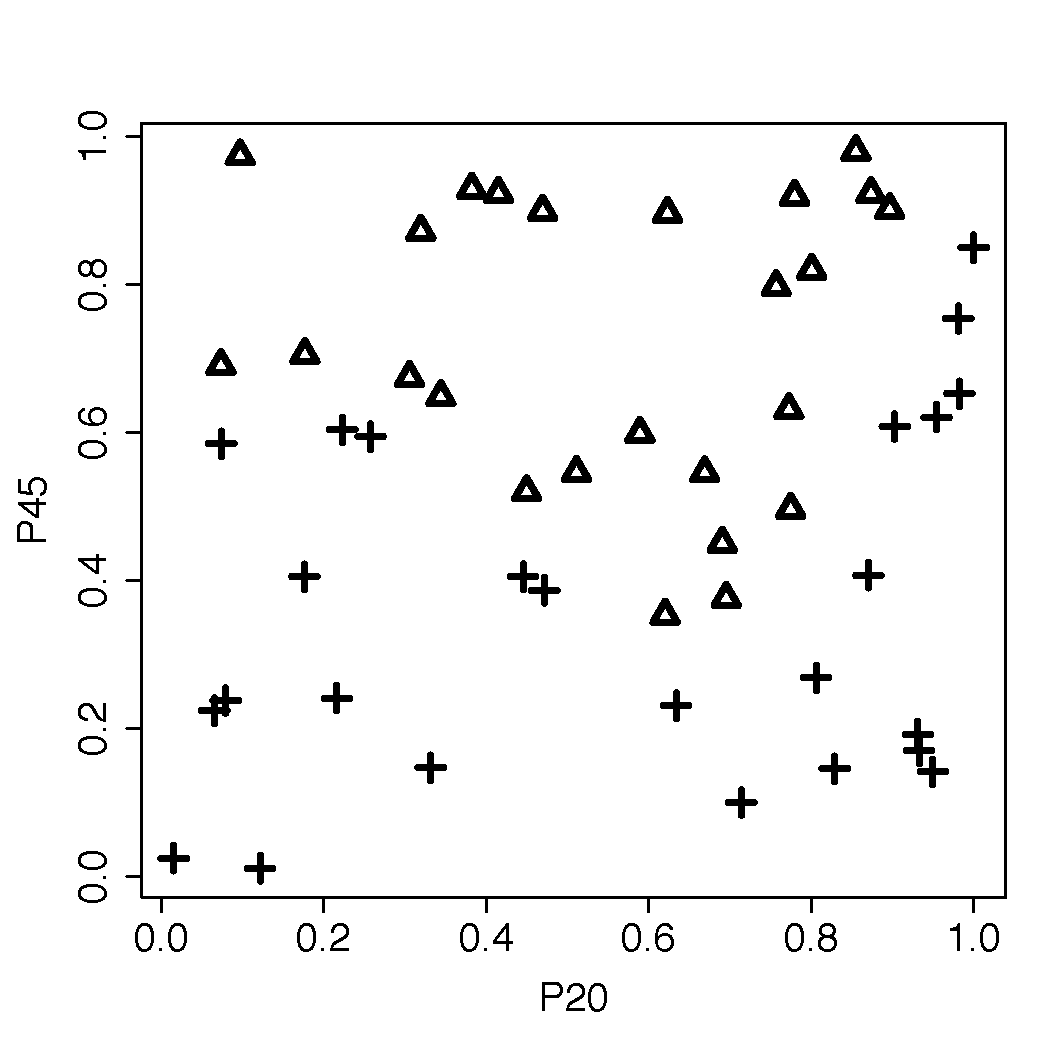
\includegraphics[width=0.65\textwidth]{./images/basisfunctionLogisticClassificationDemoDataset.pdf}
\caption{A scatter plot of the \featN{P20} and \featN{P45} features from the EEG dataset. \featL{positive} images are shown as crosses, and \featL{negative} images are shown as triangles.}
\label{fig:eegNonLinearSep}
\end{center}
\end{figure}
\end{frame} 



 \begin{frame} 
 \begin{itemize}
 	\item A logistic regression model using basis functions is defined as follows:
\end{itemize}
\begin{eqnarray}
	\mathbb{M}_{\mathbf{w}}(\mathbf{d}) & = & \frac{1}{1+e^{-\left(\displaystyle \sum_{j=0}^{b} \mathbf{w}[j]{\phi}_j(\mathbf{d})\right)}}
	\label{eqn:logisticRegressionBasisFunctions}
\end{eqnarray}
\end{frame}

\begin{frame}
 \begin{itemize}
 	\item We will use the following basis functions for the EEG problem:
\begin{tabular}[ht]{ l  l  }
$\phi_0(\mathbf{\left<\featN{P20}, \featN{P45}\right>}) =  1$ & $\phi_4(\left<\featN{P20}, \featN{P45}\right>) = \featN{P45}^2$ \\
$\phi_1(\left<\featN{P20}, \featN{P45}\right>) = \featN{P20}$ & $\phi_5(\left<\featN{P20}, \featN{P45}\right>) = \featN{P20}^3$ \\
$\phi_2(\left<\featN{P20}, \featN{P45}\right>) = \featN{P45}$ &$\phi_6(\left<\featN{P20}, \featN{P45}\right>) = \featN{P45}^3$  \\
$\phi_3(\left<\featN{P20}, \featN{P45}\right>) = \featN{P20}^2$ & $\phi_7(\left<\featN{P20}, \featN{P45}\right>) = \featN{P20} \times \featN{P45}$ \\
\end{tabular}
\end{itemize}
\end{frame} 



 \begin{frame} 
\begin{figure}[htb]
\begin{center}
	\subfigure{\label{fig:basisFunctionDemo2_1}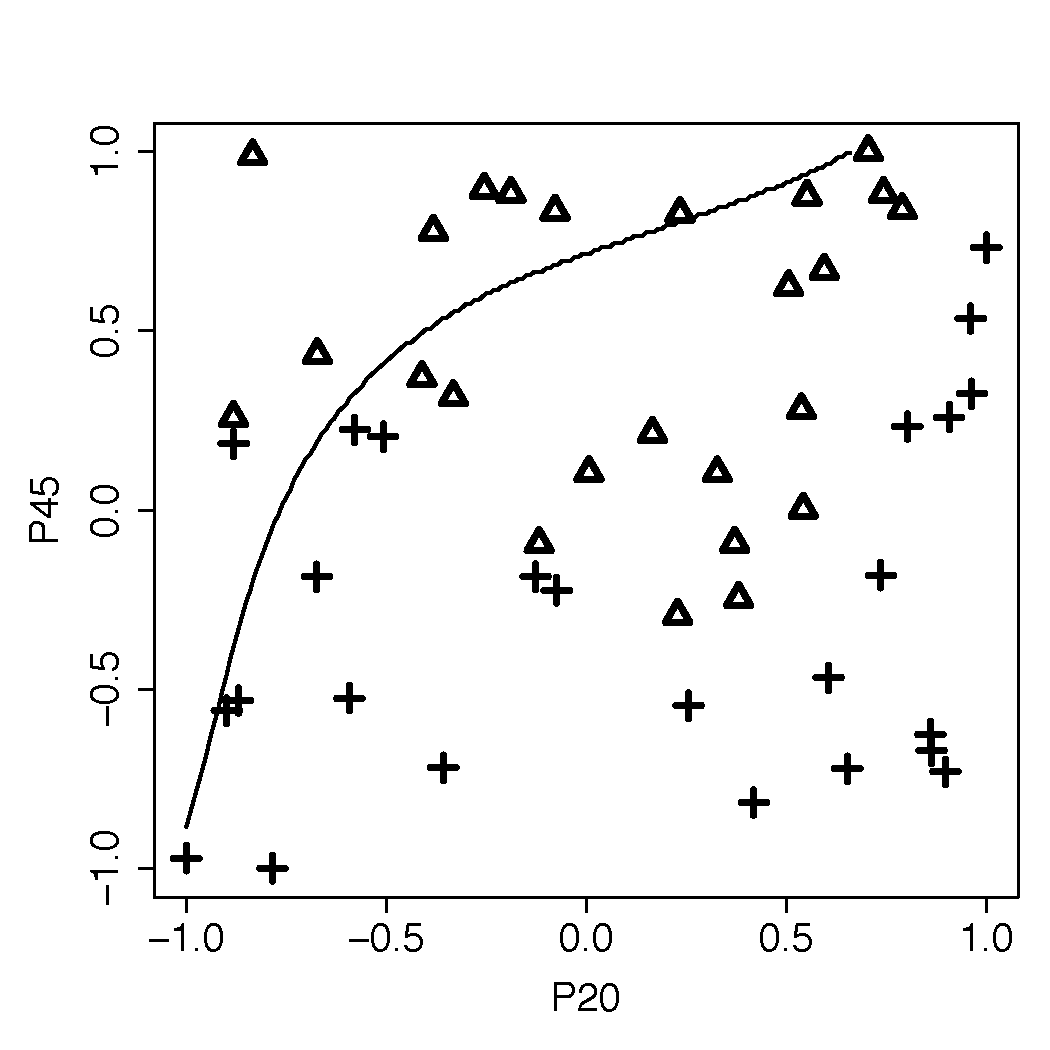
\includegraphics[width=0.27\textwidth]{./images/basisfunctionLogisticClassificationDemo0.pdf}}
	\subfigure{\label{fig:basisFunctionDemo2_3}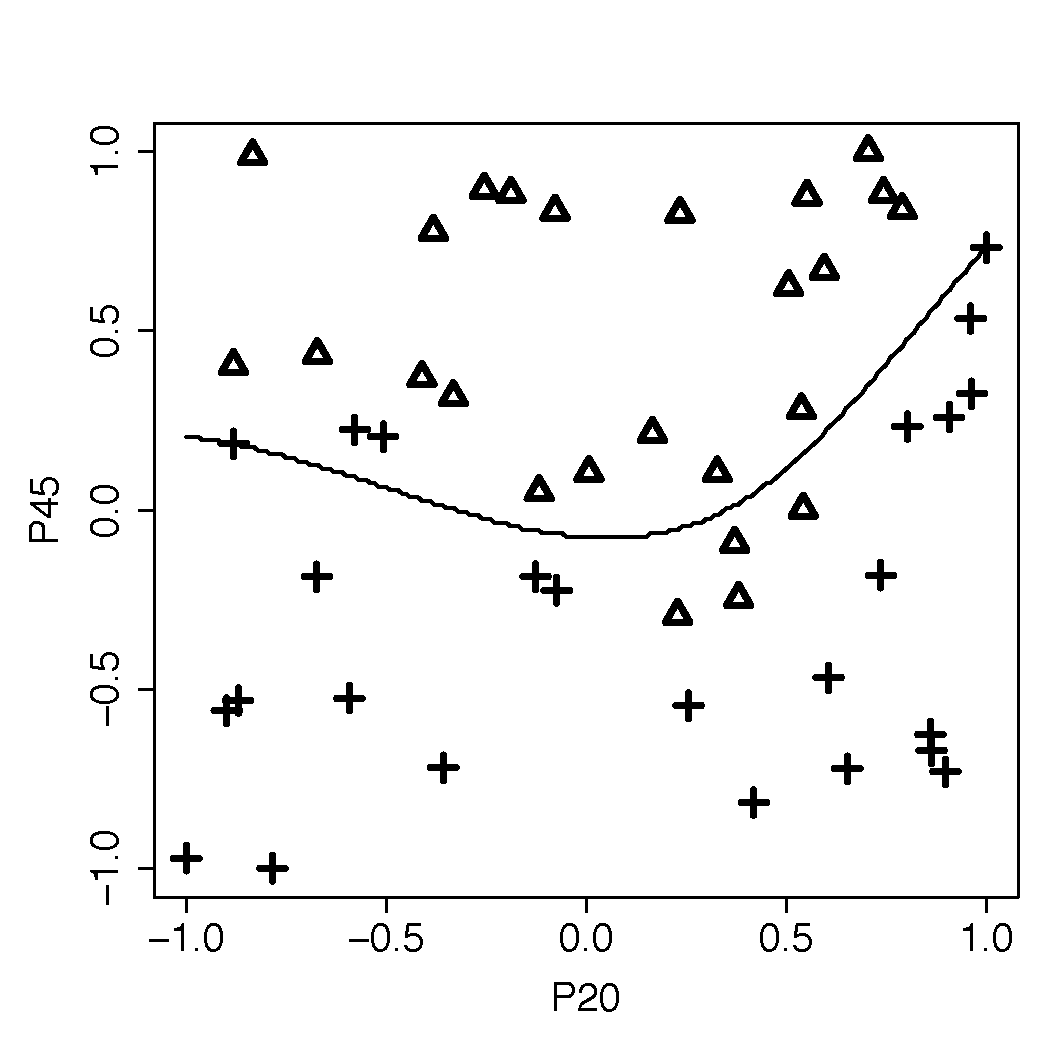
\includegraphics[width=0.27\textwidth]{./images/basisfunctionLogisticClassificationDemo9.pdf}}
	\subfigure{\label{fig:basisFunctionDemo2_4}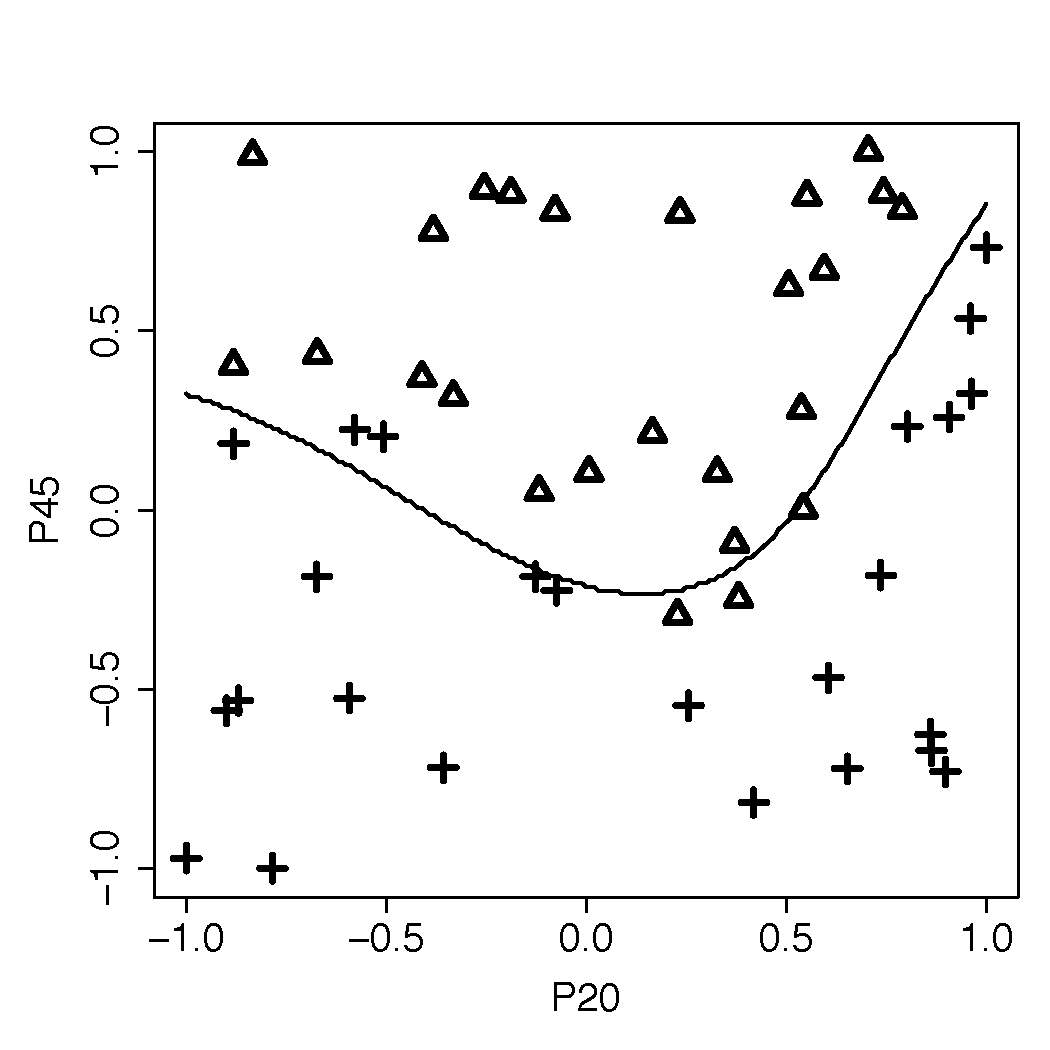
\includegraphics[width=0.27\textwidth]{./images/basisfunctionLogisticClassificationDemo25.pdf}}
	\subfigure{\label{fig:basisFunctionDemo2_7}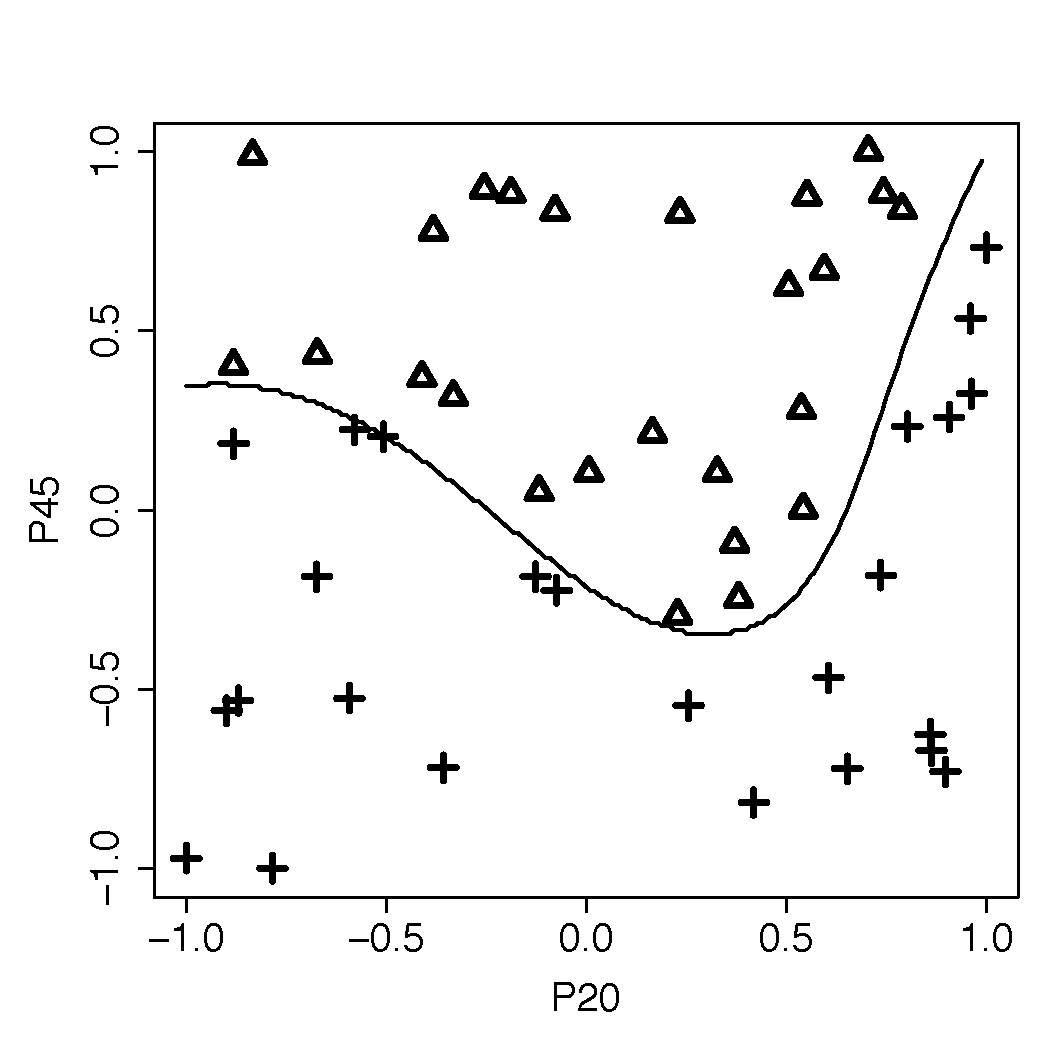
\includegraphics[width=0.27\textwidth]{./images/basisfunctionLogisticClassificationDemo214.pdf}}
	\subfigure{\label{fig:basisFunctionDemo2_9}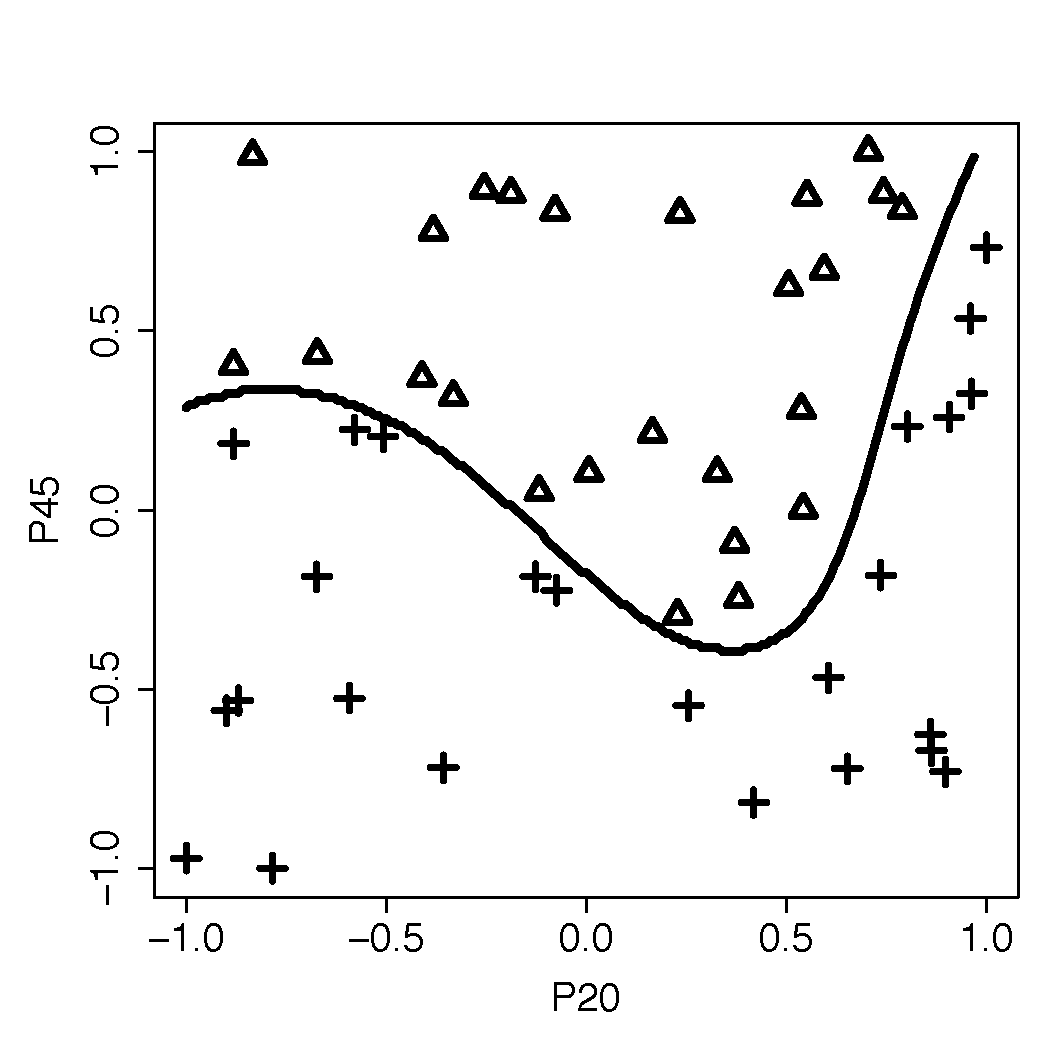
\includegraphics[width=0.27\textwidth]{./images/basisfunctionLogisticClassificationDemoFinal.pdf}}
	\subfigure{\label{fig:basisFunctionDemoDecisionSurface}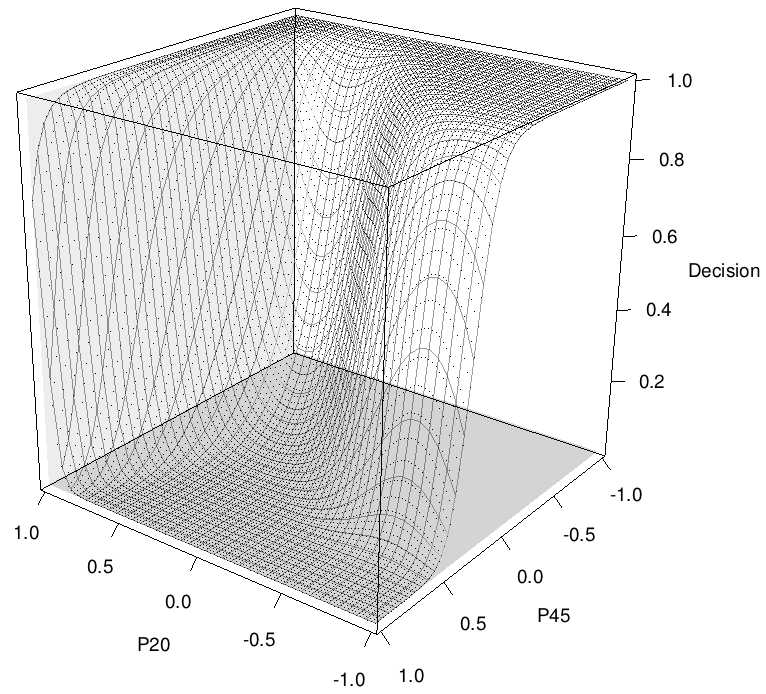
\includegraphics[width=0.27\textwidth]{./images/basisfunctionLogisticClassificationDemoDecisionSurface.png}}
\caption{A selection of the models developed during the gradient descent process for the EEG dataset from Table \ourRef{tab:eegDataset}. The final panel shows the decision surface generated.}
\label{fig:basisFunctionDemo2}
\end{center}
\end{figure}
\end{frame} 


\SectionSlideShortHeader{Multinomial Logistic Regression}{Multinomial}

 \begin{frame} 
\begin{table}[htb]
\caption{A dataset of customers of a large national retail chain.}
\label{tab:customerTypeDataset}
\centering
\begin{tiny}
\begin{tabular}{cc}
		\hline
			\begin{minipage}{0.4\textwidth}
					\begin{tabular}[ht]{ c c c c }
		\featN{ID} & \featN{Spend} & \featN{Freq} &  \featN{Type} \\
		\hline
1	&	21.6	&	5.4	&	single	\\
2	&	25.7	&	7.1	&	single	\\
3	&	18.9	&	5.6	&	single	\\
4	&	25.7	&	6.8	&	single	\\
\multicolumn{4}{c}{$\vdots$}\\
26	&	107.9	&	5.8	&	business	\\
27	&	92.9	&	5.5	&	business	\\

		\hline
					\end{tabular}
			\end{minipage}
			&
			\begin{minipage}{0.4\textwidth}
					\begin{tabular}[ht]{ c c c c }
		\featN{ID} & \featN{Spend} & \featN{Freq} &  \featN{Type} \\
		\hline
28	&	122.6	&	6.0	&	business	\\
29	&	107.7	&	5.7	&	business	\\
\multicolumn{4}{c}{$\vdots$}\\
47	&	53.2	&	2.6	&	family	\\
48	&	52.4	&	2.0	&	family	\\
49	&	46.1	&	1.4	&	family	\\
50	&	65.3	&	2.2	&	family	\\
\hline
				\end{tabular}
			\end{minipage}
\end{tabular}
\end{tiny}
\end{table}
\end{frame} 


\begin{frame}[plain] 
\begin{center}
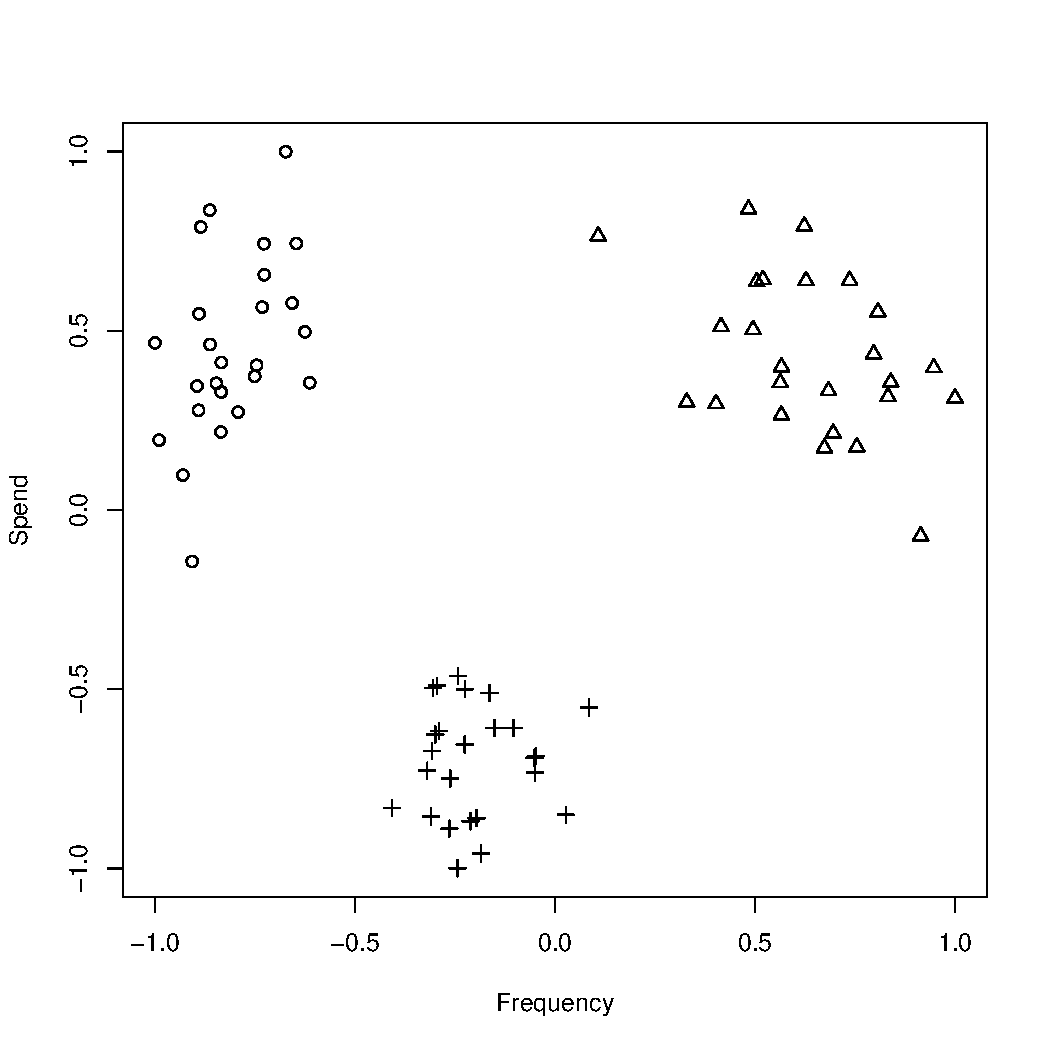
\includegraphics[width=0.65\textwidth]{./images/gradientDescentMultinomialLogisticClassificationDemoDataset.pdf}
\end{center}
\end{frame} 

\begin{frame} 
\begin{figure}[htb]
\begin{center}
	\subfigure[]{\label{fig:multinomialOneVersusAllExplanation0}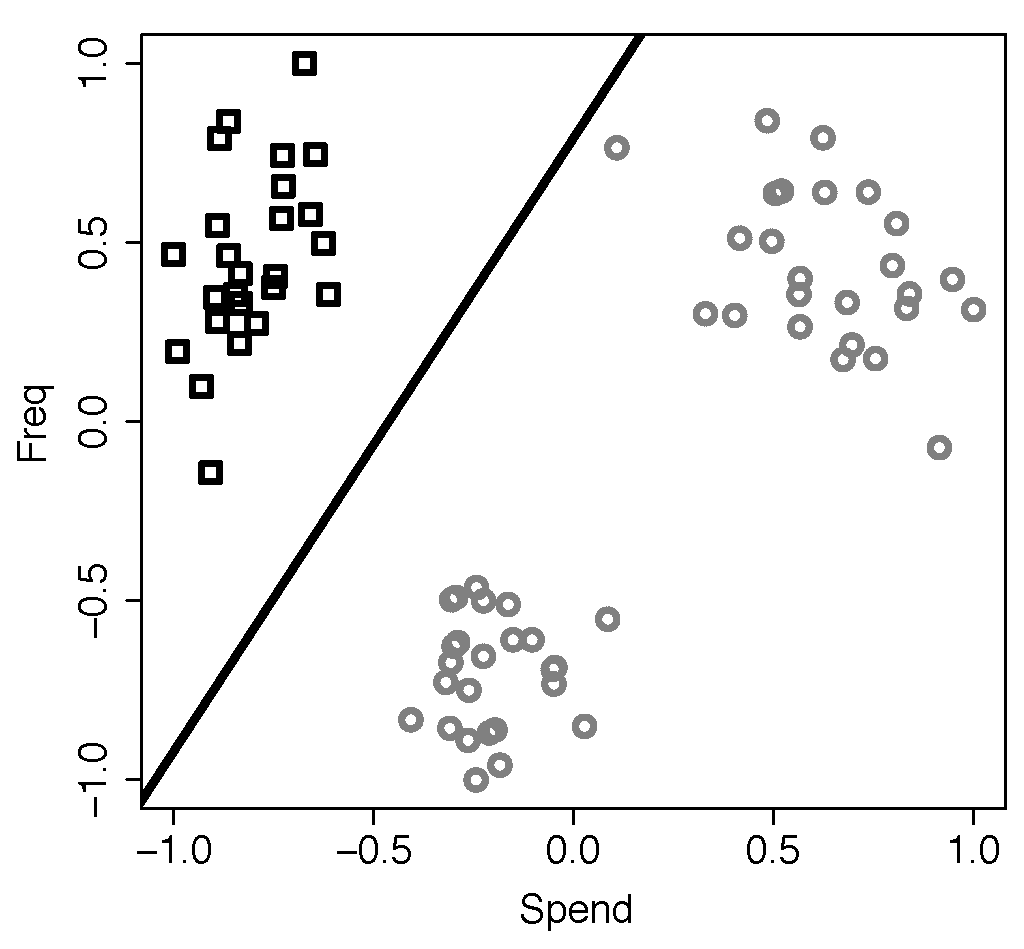
\includegraphics[width=0.32\textwidth]{./images/gradientDescentMultinomialLogisticClassificationDemoOneVersusall0_mod.pdf}}
	\subfigure[]{\label{fig:multinomialOneVersusAllExplanation1}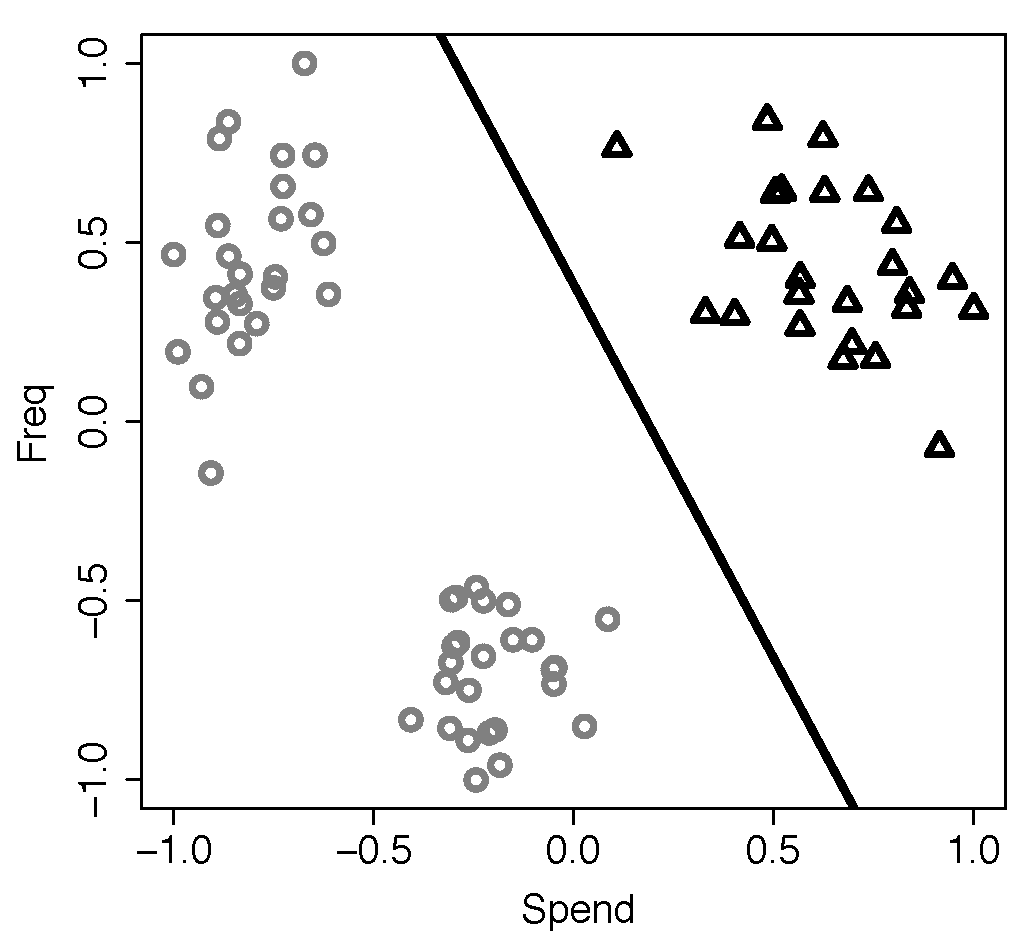
\includegraphics[width=0.32\textwidth]{./images/gradientDescentMultinomialLogisticClassificationDemoOneVersusall1_mod.pdf}}
	\subfigure[]{\label{fig:multinomialOneVersusAllExplanation2}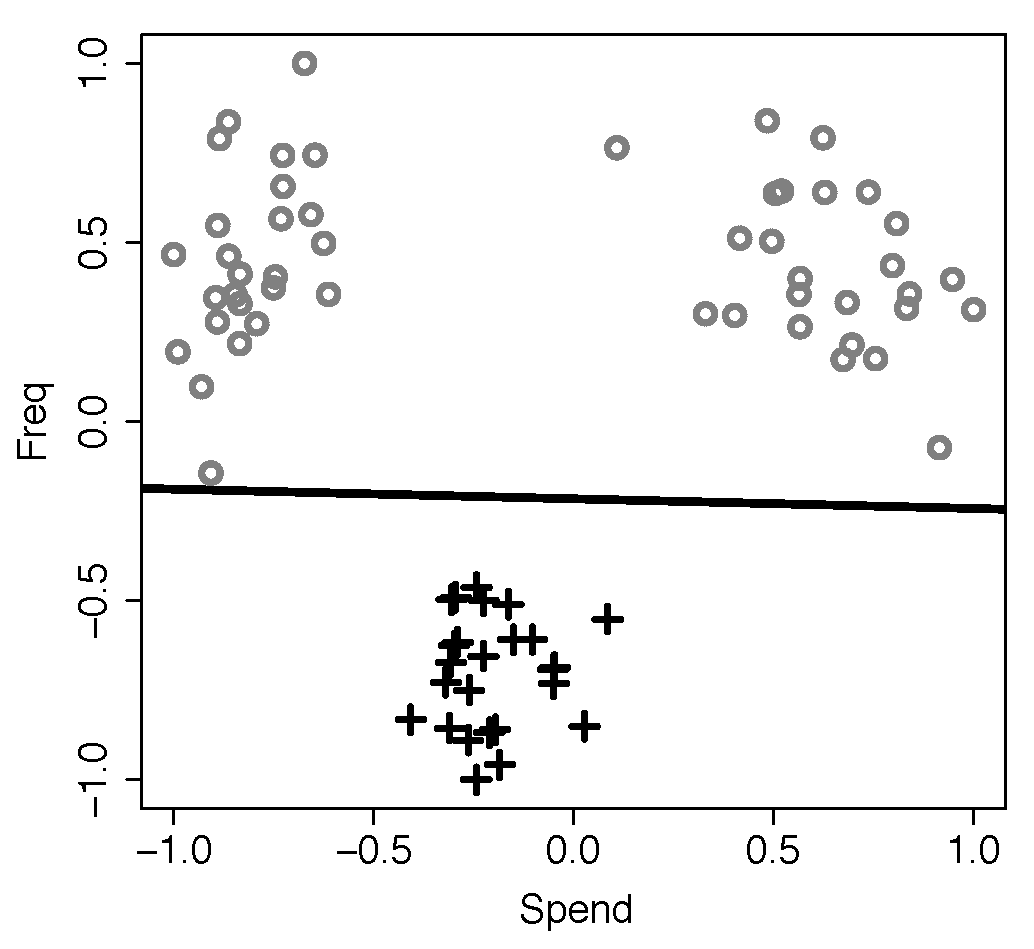
\includegraphics[width=0.32\textwidth]{./images/gradientDescentMultinomialLogisticClassificationDemoOneVersusall2_mod.pdf}}
\caption{An illustration of three different \indexkeyword{one-versus-all} prediction models for the customer type dataset in Table \ourRef{tab:customerTypeDataset} that has three target levels \featL{single} (squares), \featL{business} (triangles) and \featL{family} (crosses).}
\label{fig:multinomialOneVersusAllExplanation}
\end{center}
\end{figure}
\end{frame} 



\begin{frame} 
\begin{itemize}
\item For $r$  target feature levels, we build $r$ separate logistic regression models $\mathbb{M}_{\mathbf{w_1}}$ to $\mathbb{M}_{\mathbf{w_r}}$:
\begin{equation}
	\begin{alignedat}{2}
	\mathbb{M}_{\mathbf{w_1}}(\mathbf{d}) & = logistic(\mathbf{w_1} \cdot \mathbf{d}) \\
	\mathbb{M}_{\mathbf{\mathbf{w_2}}}(\mathbf{d}) & = logistic(\mathbf{\mathbf{w_2}} \cdot \mathbf{d}) \\
	&  \vdots \\
	\mathbb{M}_{\mathbf{w_r}}(\mathbf{d}) & = logistic(\mathbf{w_r} \cdot \mathbf{d}) \\
	\end{alignedat}
\label{eqn:multinomialLogisticRegression}
\end{equation}
\noindent where $\mathbb{M}_{\mathbf{w_1}}$ to $\mathbb{M}_{\mathbf{w_r}}$ are $r$ different one-versus-all logistic regression models, and $\mathbf{w_1}$ to $\mathbf{w_r}$ are $r$ different sets of weights.
\end{itemize}
\end{frame} 


\begin{frame} 
\begin{itemize}
\item To combine the outputs of these different models, we normalize their results using: 
\begin{equation}
	\begin{alignedat}{2}
		\mathbb{M}'_{\mathbf{w_k}}(\mathbf{d}) = \frac{\mathbb{M}_{\mathbf{w_k}}(\mathbf{d})}{\displaystyle\sum_{l \in levels(t)}\mathbb{M}_{\mathbf{w}_l}(\mathbf{d})} 
	\end{alignedat}
\label{eqn:softmax}
\end{equation}
\noindent where $\mathbb{M}'_{\mathbf{w_k}}(\mathbf{d})$ is a revised, normalized prediction for the one-versus-all model for the target level $k$. 
\end{itemize}
\end{frame} 



\begin{frame} 
\begin{itemize}
\item The $r$ one-versus-all logistic regression models used are trained in \alert{parallel}, and the \alert{revised model outputs}, $\mathbb{M}'_{\mathbf{w_k}}(\mathbf{d})$, are used when calculating the sum of squared errors for each model during the training process.  
\item This means that the sum of squared errors function is changed slightly to
\begin{alignat}{2}
L_2(\mathbb{M}_{\mathbf{w_k}}, \mathcal{D}) & = \frac{1}{2} \sum_{i=1}^{n} \left(t_i - \mathbb{M}'_{\mathbf{w_k}}(\mathbf{d}_i\left[1\right])\right)^2 
\end{alignat}
\end{itemize}
\end{frame} 

\begin{frame} 
\begin{itemize}
\item The revised predictions are also used when making predictions for query instances. The predicted level for a query, $\mathbf{q}$, is the level associated with the one-versus-all model that outputs the highest result after normalization. 
\item We can write this as
\begin{alignat}{2}
\mathbb{M}(\mathbf{q}) &= \argmax_{l \in levels(t)} \mathbb{M}'_{\mathbf{w}_l}(\mathbf{q})
\end{alignat}
\end{itemize}
\end{frame} 

 \begin{frame}[plain]
\begin{figure}[!bth]
\begin{center}\subfigure{\label{fig:multinomialRegresionDemo2}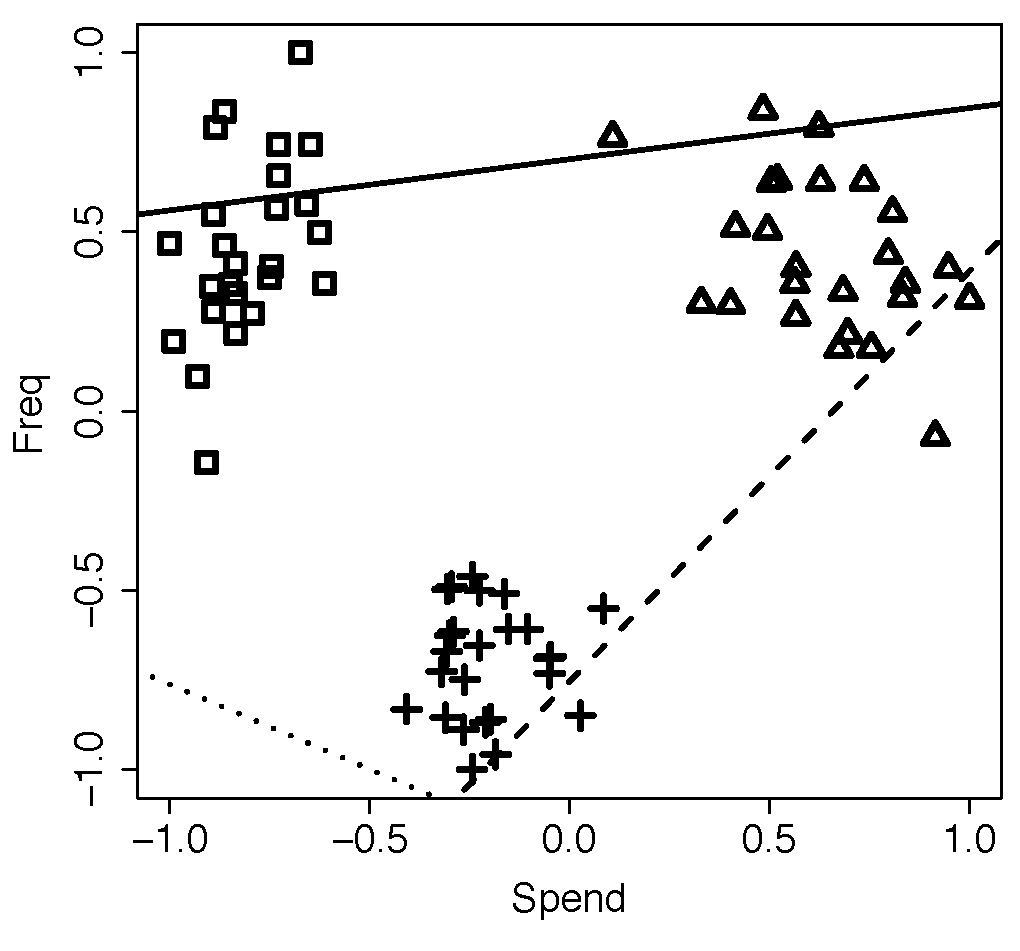
\includegraphics[width=0.27\textwidth]{./images/gradientDescentMultinomialLogisticClassificationDemo2.pdf}}
\subfigure{\label{fig:multinomialRegresionDemo3}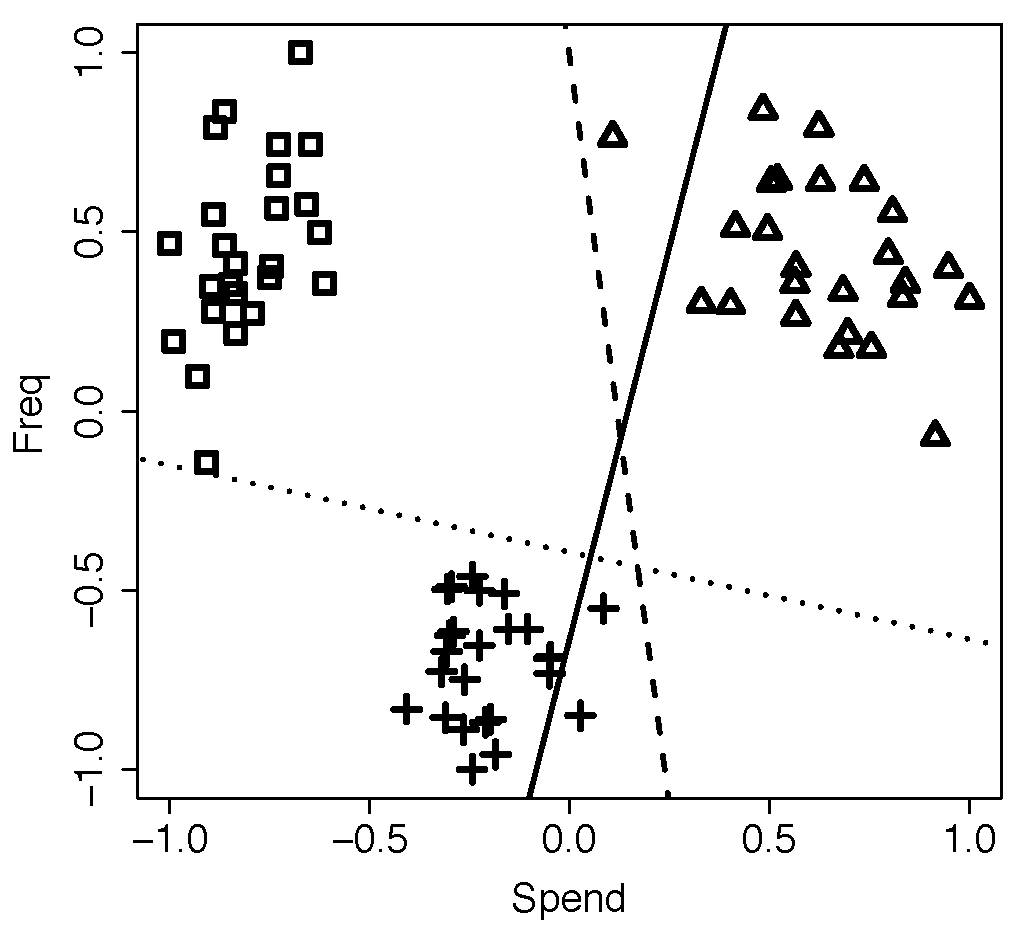
\includegraphics[width=0.27\textwidth]{./images/gradientDescentMultinomialLogisticClassificationDemo20.pdf}}	
\subfigure{\label{fig:multinomialRegresionDemo4}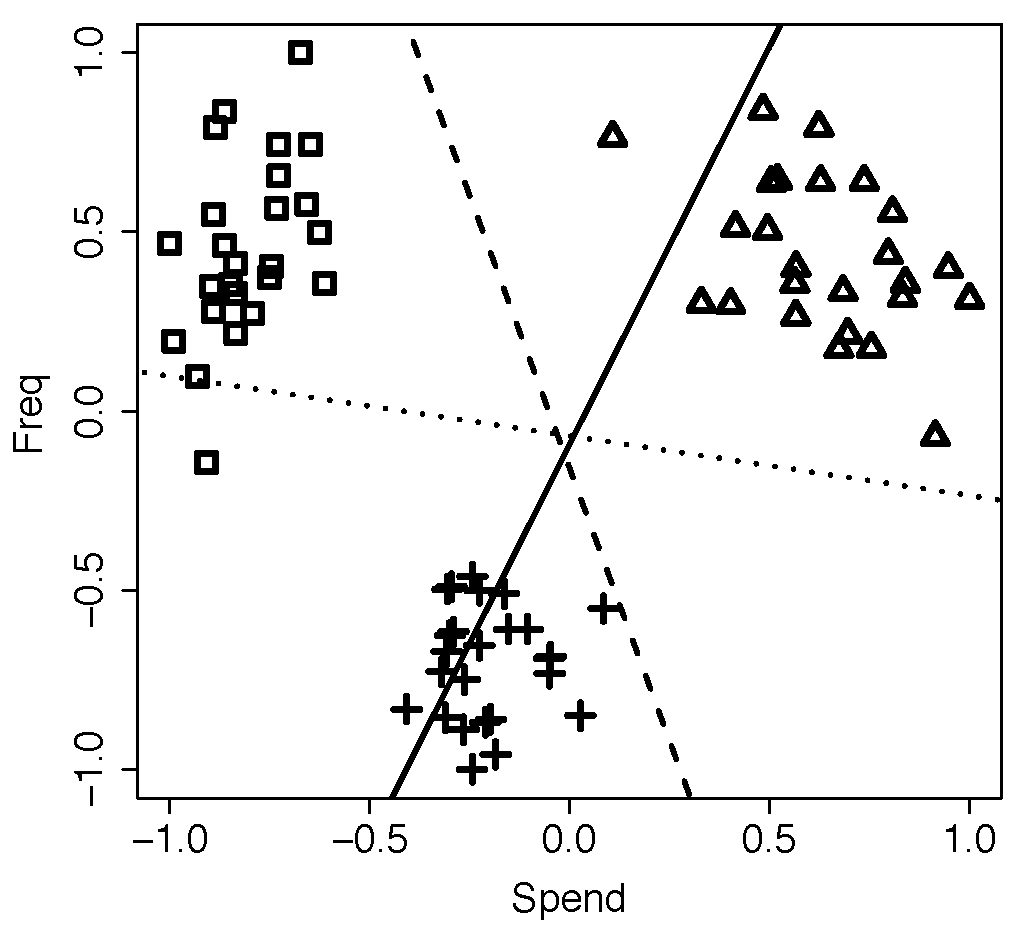
\includegraphics[width=0.27\textwidth]{./images/gradientDescentMultinomialLogisticClassificationDemo50.pdf}}
\subfigure{\label{fig:multinomialRegresionDemo7}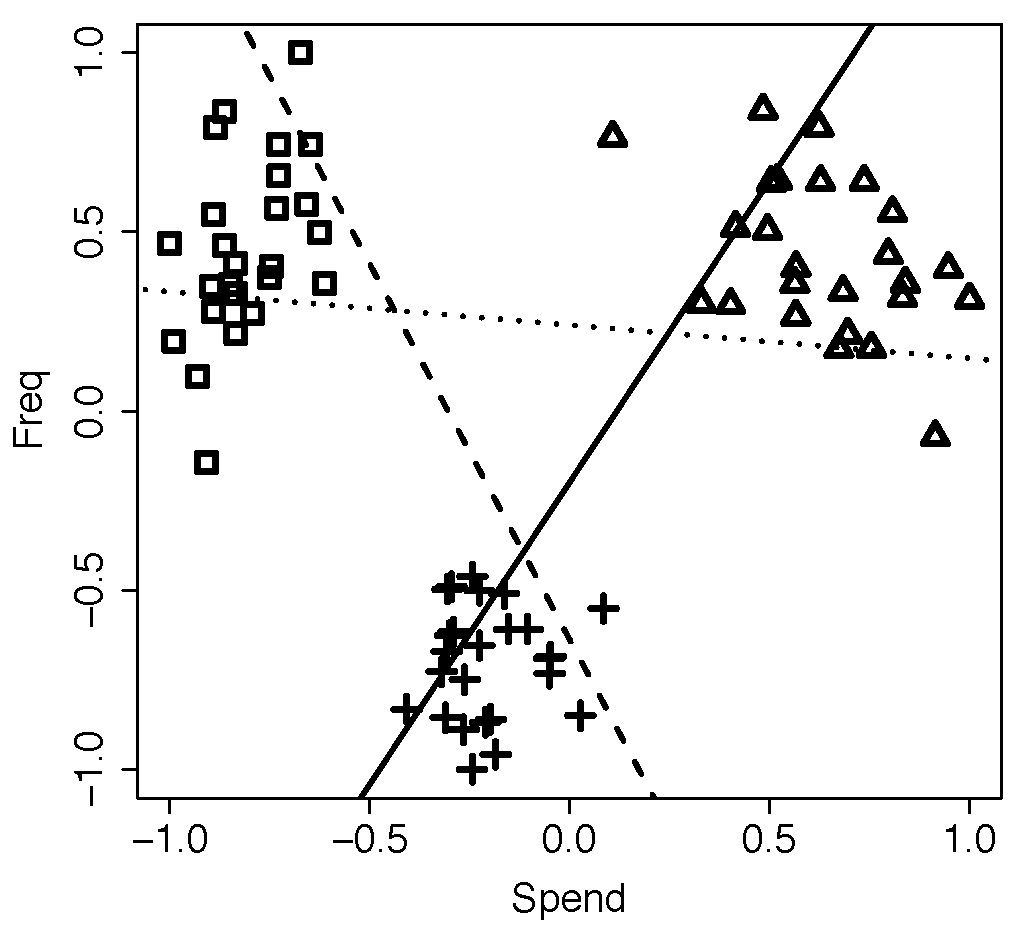
\includegraphics[width=0.27\textwidth]{./images/gradientDescentMultinomialLogisticClassificationDemo309.pdf}}
\subfigure{\label{fig:multinomialRegresionDemo9}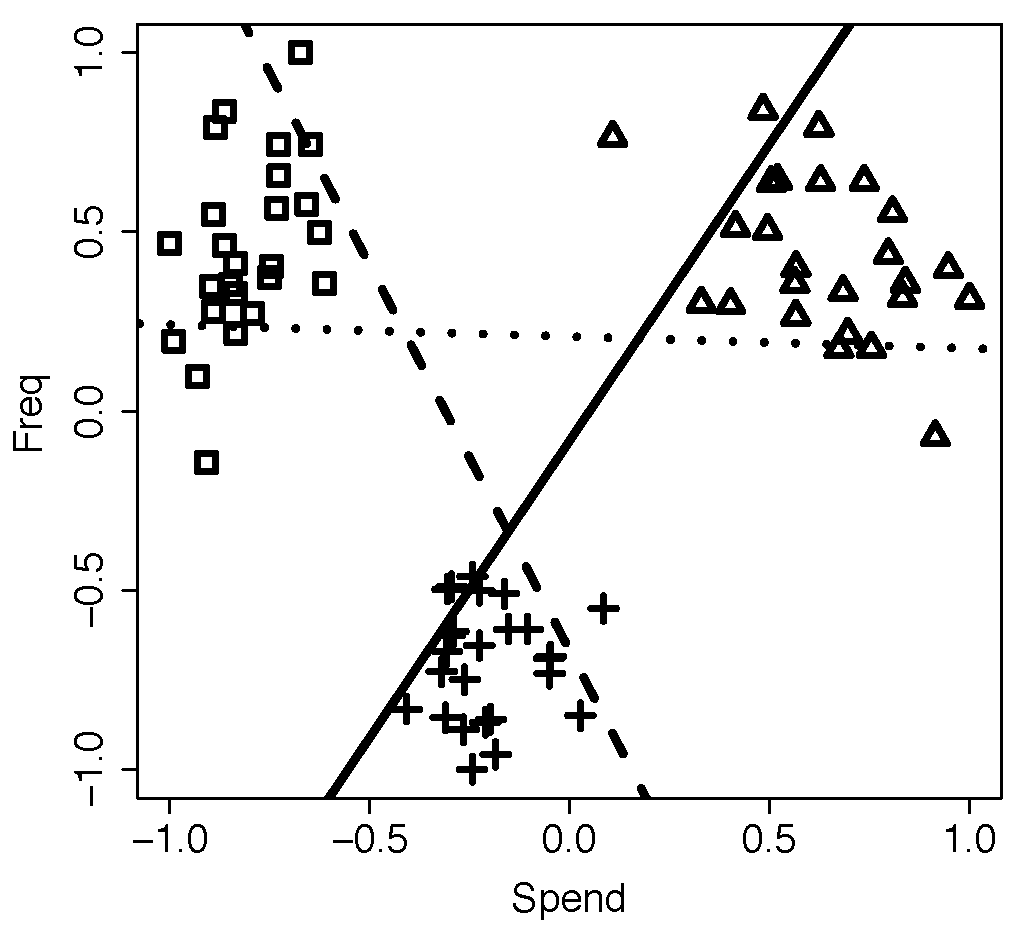
\includegraphics[width=0.27\textwidth]{./images/gradientDescentMultinomialLogisticClassificationDemoFinal.pdf}}
\subfigure{\label{fig:multinomialRegresionDemoBoundary}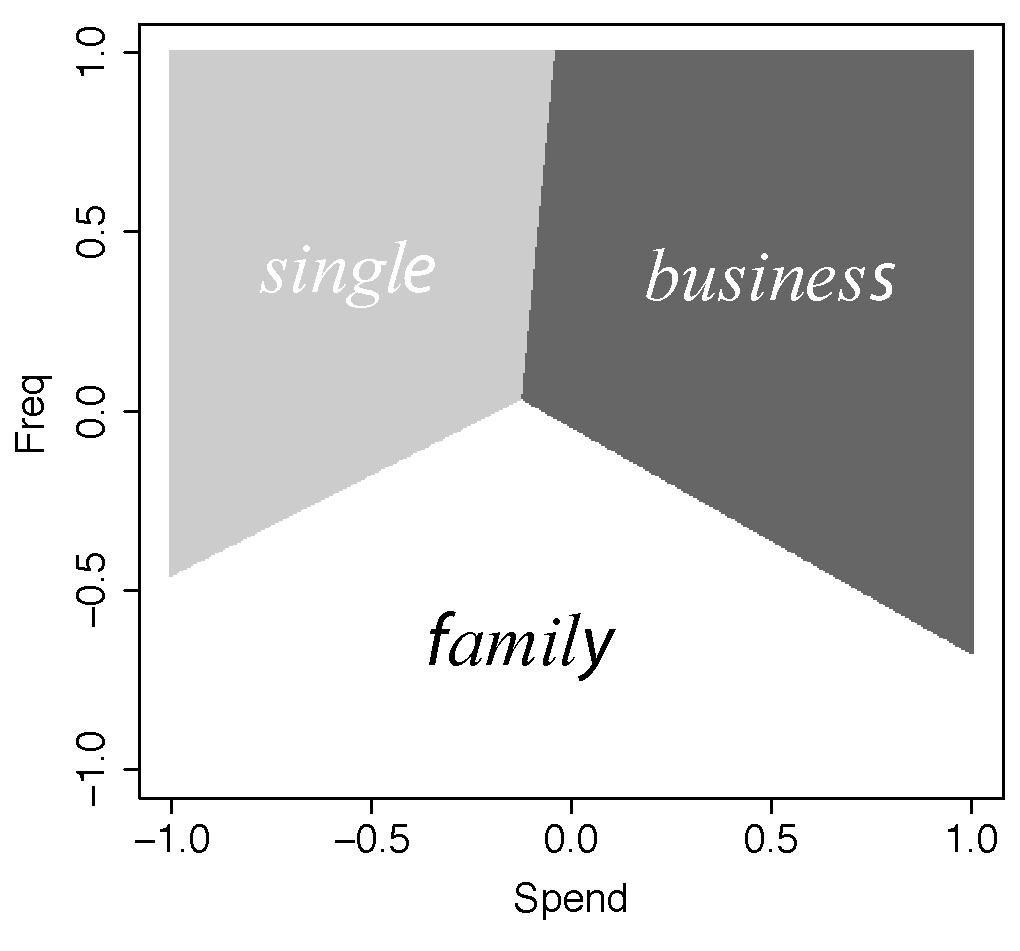
\includegraphics[width=0.27\textwidth]{./images/gradientDescentMultinomialLogisticClassificationDemoDatasetDecisionBoundary.pdf}}	
\caption{A selection of the models developed during the gradient descent process for the customer group dataset from Table \ourRef{tab:customerTypeDataset}. Squares represent instances with the \featL{single} target level, triangles the \featL{business} level and crosses the \featL{family} level. (f) illustrates the overall decision boundaries that are learned between the three target levels.}
\label{fig:multinomialRegresionDemo}
\end{center}
\end{figure}
\end{frame} 

 \begin{frame}[plain]
\begin{center}
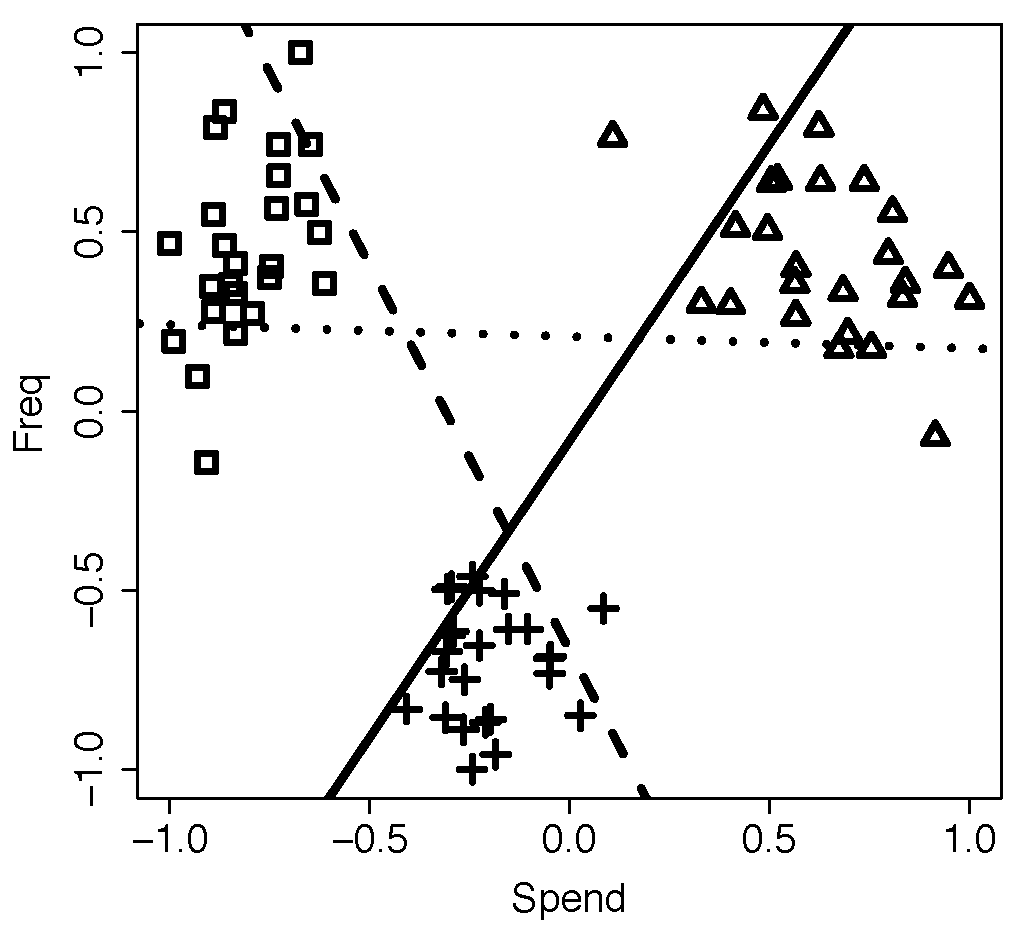
\includegraphics[width=0.55\textwidth]{./images/gradientDescentMultinomialLogisticClassificationDemoFinal.pdf}
\end{center}
\begin{equation*}
\mathbb{M}_{\mathbf{w_{\featL{single}}}}(\mathbf{q})  = Logistic(0.7993 - 15.9030\times\featN{Spend} + 9.5974\times\featN{Freq}) 
\end{equation*}
\begin{equation*}
	\mathbb{M}_{\mathbf{w_{\featL{family}}}}(\mathbf{q})  = Logistic(3.6526 + -0.5809\times\featN{Spend} - 17.5886\times\featN{Freq}) 
\end{equation*}
\begin{equation*}
	\mathbb{M}_{\mathbf{w_{\featL{business}}}}(\mathbf{q})  = Logistic(4.6419 + 14.9401\times\featN{Spend} - 6.9457\times\featN{Freq}) 
\end{equation*}
\end{frame} 

 \begin{frame} 
\begin{itemize}
\begin{footnotesize}
\item For a query instance with $\featN{Spend} =25.67$ and $\featN{Freq} = 6.12$, which are normalized to $\featN{Spend} =-0.7279$ and $\featN{Freq} = 0.4789$, the predictions of the individual models would be
\begin{equation*}
	\begin{alignedat}{2}
	\mathbb{M}_{\mathbf{w_{\featL{single}}}}(\mathbf{q}) & = Logistic(0.7993 - 15.9030\times(-0.7279) + 9.5974\times0.4789) \\
	& = 0.9999 \\
	\mathbb{M}_{\mathbf{w_{\featL{family}}}}(\mathbf{q}) & = Logistic(3.6526 + -0.5809\times(-0.7279) - 17.5886\times0.4789) \\
		& = 0.01278 \\
	\mathbb{M}_{\mathbf{w_{\featL{business}}}}(\mathbf{q}) & = ?
\end{alignedat}
\end{equation*}
\end{footnotesize}
\end{itemize}
\end{frame} 

 \begin{frame} 
\begin{itemize}
\begin{footnotesize}
\item For a query instance with $\featN{Spend} =25.67$ and $\featN{Freq} = 6.12$, which are normalized to $\featN{Spend} =-0.7279$ and $\featN{Freq} = 0.4789$, the predictions of the individual models would be
\begin{equation*}
	\begin{alignedat}{2}
	\mathbb{M}_{\mathbf{w_{\featL{single}}}}(\mathbf{q}) & = Logistic(0.7993 - 15.9030\times(-0.7279) + 9.5974\times0.4789) \\
	& = 0.9999 \\
	\mathbb{M}_{\mathbf{w_{\featL{family}}}}(\mathbf{q}) & = Logistic(3.6526 + -0.5809\times(-0.7279) - 17.5886\times0.4789) \\
		& = 0.01278 \\
	\mathbb{M}_{\mathbf{w_{\featL{business}}}}(\mathbf{q}) & = Logistic(4.6419 + 14.9401\times(-0.7279) - 6.9457\times0.4789) \\
		& = 0.0518 \\
\end{alignedat}
\end{equation*}
\end{footnotesize}
\end{itemize}
\end{frame} 



 \begin{frame} 
 \begin{itemize}
 \item These predictions would be normalized as follows:
\begin{equation*}
	\begin{alignedat}{2}
	\mathbb{M}'_{\mathbf{w_{\featL{single}}}}(\mathbf{q}) & = \frac{0.9999}{0.9999 + 0.01278 + 0.0518} = 0.9393\\
	\mathbb{M}'_{\mathbf{w_{\featL{family}}}}(\mathbf{q}) & = \frac{0.01278}{0.9999 + 0.01278 + 0.0518} = 0.0120\\
	\mathbb{M}'_{\mathbf{w_{\featL{business}}}}(\mathbf{q}) & = \frac{0.0518}{0.9999 + 0.01278 + 0.0518} = 0.0487\\
\end{alignedat}
\end{equation*}
\item This means the overall prediction for the query instance is \featL{single}, as this gets the highest normalized score.
\end{itemize}
\end{frame} 


\SectionSlideShortHeader{Support Vector Machines}{SVM}

 \begin{frame}[plain]
 \begin{center}
\begin{figure}[htb]
\includegraphics[width=0.65\textwidth]{./images/svmBadMarginImage.pdf}
\caption{A small sample of the generators dataset with two features, \featN{RPM} and \featN{Vibration}, and two target levels, \featL{good} (shown as crosses) and \featL{bad} (shown as triangles). A decision boundary with a very small margin.}
\label{fig:svmDemoBad}
\end{figure}
\end{center}
\end{frame} 

 \begin{frame}[plain] 
 \begin{center}
\begin{figure}[htb]
\includegraphics[width=0.65\textwidth]{./images/svmGoodMarginImage}
\caption{A small sample of the generators dataset with two features, \featN{RPM} and \featN{Vibration}, and two target levels, \featL{good} (shown as crosses) and \featL{bad} (shown as triangles). A decision boundary with a large margin.}
\label{fig:svmDemoGood}
\end{figure}
\end{center}
\end{frame} 

 \begin{frame}
 \begin{itemize}
 \item Training a  support vector machine involves searching for the decision boundary, or \keyword{separating hyperplane}, that leads to the maximum margin as this will best separate the levels of the target feature. 
 \item The instances in a training dataset that fall along the margin extents, and so define the margins, are known as the \keyword{support vectors} and define the decision boundary. 
 \end{itemize}
\end{frame} 

\begin{frame} 
\begin{itemize}
\item We define the separating hyperplane as follows:
\begin{alignat}{1}
w_0 + \mathbf{w} \cdot \mathbf{d} = 0
\label{eqn:basicSVMBoundary}
\end{alignat}
\item For instances above a separating hyperplane
\begin{alignat*}{1}
w_0 + \mathbf{w} \cdot \mathbf{d} > 0
\end{alignat*}
\noindent and for instances below a separating hyperplane
\begin{alignat*}{1}
w_0 + \mathbf{w} \cdot \mathbf{d} < 0
\end{alignat*}
\end{itemize}
\end{frame}

\begin{frame}
\begin{itemize}
\item We build a support vector machine prediction model so that instances with the negative target level result in the model outputting $\le-1$ and instances with the positive target level result in the model outputting $\ge+1$. 
\item The space between the outputs of $-1$ and $+1$ allows for the margin.
\end{itemize}
\end{frame} 




 \begin{frame} 
 \begin{itemize}
\item A support vector machine model is defined as
\begin{alignat}{1}
\mathbb{M}_{\pmb{\alpha}, w_0}(\mathbf{q}) = \displaystyle \sum_{i=1}^{s} \left(t_i\times\pmb{\alpha}[i]\times\left(\mathbf{d}_i \cdot \mathbf{q}\right) + w_0 \right) 
\label{eqn:svmPredictionEquation}
\end{alignat}
\noindent where 
	\item $\mathbf{q}$ is the set of descriptive features for a query instance; 
	\item $(\mathbf{d}_1, t_1), \ldots, (\mathbf{d}_s, t_s)$ are $s$ support vectors (instances composed of descriptive features and a target feature); 
	\item $w_0$ is the first weight of the decision boundary; 
	\item and $\pmb{\alpha}$ is a set of parameters determined during the training process (there is a parameter for each support vector $\pmb{\alpha}\left[1\right], \ldots, \pmb{\alpha}\left[s\right]$).\footnote{These parameters are formally known as \keyword{Lagrange multipliers}.} 
\end{itemize}
\end{frame} 

 \begin{frame} 
 \begin{itemize}
\item Training a support vector machine is frames as a \keyword{constrained quadratic optimization problem}
\item This type of problem is defined in terms of:
\begin{enumerate}
	\item a set of constraints
	\item an optimization criterion. 
\end{enumerate}
\end{itemize}
\end{frame} 


 \begin{frame} 
 \begin{itemize}
\item The required \keyword{constraints} required by the training process are
\begin{alignat}{4}
w_0 + \mathbf{w}\cdot\mathbf{d} & \le &-1  & \text{~for~} t_i = -1\label{eqn:svmConstraint1}
\intertext{and:}
w_0 + \mathbf{w}\cdot\mathbf{d} & \ge & +1 & \text{~for~} t_i = +1 \label{eqn:svmConstraint2}
\end{alignat}
\item We can combine these two constraints into a single constraint (remember $t_i$ is always equal to either $-1$ or $+1$):
\begin{alignat}{4}
t_i\times(w_0 + \mathbf{w}\cdot\mathbf{d}) & \ge &\;1 \label{eqn:svmCombinedConstraint}
\end{alignat}
\end{itemize}
\end{frame} 


 \begin{frame} 
\begin{figure}
\centering
	\subfigure[]{\label{fig:svmDemoAlternate1}\includegraphics[width=0.4\textwidth]{./images/svmAlternativeMarginImage1.pdf}}
		\subfigure[]{\label{fig:svmDemoQueries}\includegraphics[width=0.4\textwidth]{./images/svmQueriesImage.pdf}}
\caption{Different margins that satisfy the constraint in Equation \ourEqRef{eqn:svmCombinedConstraint}. The instances that define the margin are highlighted in each case. (b) shows the maximum margin and also shows two query instances represented as black dots.}
\label{fig:svmDemoMargins}
\end{figure}
\end{frame} 


\begin{frame}
\begin{itemize}
\item The \keyword{optimization} criterion used is defined in terms of the perpendicular distance from any instance to the decision boundary and is given by
\begin{alignat*}{1}
dist(\mathbf{d}) = \displaystyle\frac{w_0 + abs(\mathbf{w}\cdot \mathbf{d})}{||\mathbf{w}||}
\end{alignat*}
\noindent where $||\mathbf{w}||$ is known as the \keyword{Euclidean norm} of  $\mathbf{w}$ and is calculated as
\begin{alignat*}{1}
||\mathbf{w}|| = \sqrt{\mathbf{w}\left[1\right]^2 + \mathbf{w}\left[2\right]^2 + \ldots + \mathbf{w}\left[m\right]^2}
\end{alignat*}
\item For instances along the \indexkeyword{margin extents}, $abs(\mathbf{w}\cdot \mathbf{d} + w_0) = 1$. 
\item So, the distance from any instance along the margin extents to the decision boundary is $ \frac{1}{||\mathbf{w}||}$, and because the margin is symmetrical to either side of the decision boundary, the size of the margin is $ \frac{2}{||\mathbf{w}||}$. 
\end{itemize}
\end{frame} 

 \begin{frame} 
 \begin{itemize}
\item The goal when training a support vector machine is
\begin{enumerate}
	\item \alert{maximize} $ \frac{2}{||\mathbf{w}||}$ 
	\item \alert{subject to the constraint} 
\end{enumerate}
\end{itemize}
\begin{equation*}
t_i\times(w_0 + \mathbf{w}\cdot\mathbf{d})  \ge \;1
\end{equation*}
\end{frame} 

 \begin{frame} 
\begin{center}
 \includegraphics[width=0.4\textwidth]{./images/svmQueriesImage.pdf}
 \end{center}
\begin{itemize}  
\item The optimal decision boundary and associated support vectors for the example we have been following 
\item In this case  \featL{good} is the positive level and set to $+1$, and \featL{faulty} is the negative level and set to $-1$. 
\end{itemize}
\end{frame}

\begin{frame}
\begin{itemize}
\item The descriptive feature values and target feature values for the support vectors in these cases are
\begin{itemize}
	\item  $(\left< -0.225, 0.217 \right>, +1)$, 
	\item $(\left<-0.066, -0.069\right>, -1)$, 
	\item $(\left<-0.273, -0.080\right>, -1)$. 
\end{itemize}
\item The value of $w_0$ is $-0.1838$, 
\item The values of the $\pmb{\alpha}$ parameters are 
\end{itemize}
\begin{center}
$\left< 22.056, 6.998, 16.058 \right>$. 
\end{center}
\end{frame} 

 \begin{frame} 
 \begin{center}
 \includegraphics[width=0.4\textwidth]{./images/svmQueriesImage.pdf}
 \end{center}
  \begin{itemize}
\item The plot shows the position of two new query instances for this problem. 
\item The descriptive feature values for these querys are
\begin{enumerate}
	\item $\mathbf{q_1} = \left<-0.314, -0.251\right>$ 
	\item $\mathbf{q_2} = \left<-0.117, 0.31\right>$. 
\end{enumerate}
\end{itemize}
\end{frame}

\begin{frame}
\begin{itemize}
\item For the first query instance,  $\mathbf{q_1}= \left<-0.314, -0.251\right>$,  the output of the support vector machine model is:
\begin{footnotesize}
\begin{alignat*}{2}
\mathbb{M}_{\pmb{\alpha}, w_0}&(\mathbf{q_1}) \\
 = & \left(1 \times 23.056 \times \left(\left(-0.225 \times -0.314\right) + \left(0.217 \times -0.251\right)\right) -0.1838 \right) \\
 & + \left(-1 \times 6.998 \times \left(\left(-0.066 \times -0.314\right) + \left(-0.069 \times -0.251\right)\right) -0.1838 \right) \\
  & + \left(-1 \times 16.058 \times \left(\left(-0.273 \times -0.314\right) + \left(-0.080 \times -0.251\right)\right) -0.1838 \right) \\
   = & -2.145 
\end{alignat*}
\end{footnotesize}
\item The model output is less than $-1$, so this query is predicted to be a \featL{faulty} generator. 
\item For the second query instance, the model output is $1.592$, so this instance is predicted to be a \featL{good} generator.
\end{itemize}
\end{frame} 



 \begin{frame} 
  \begin{itemize}
\item \keyword{Basis functions} can be used with support vector machines to handle data that is not \indexkeyword{linearly separable}
\item To use basis functions we update Equation \ourEqRef{eqn:svmCombinedConstraint} to
\begin{alignat}{4}
t_i\times(w_0 + \mathbf{w}\cdot\pmb{\phi}\left(\mathbf{d}\right)) & \ge &\;1  & \text{~for all~} i \label{eqn:svmCombinedConstraintNonLinear}
\end{alignat}
\noindent where $\pmb{\phi}$ is a set of basis functions applied to the descriptive features $\mathbf{d}$, and $\mathbf{w}$ is a set of weights containing one weight for each member of $\pmb{\phi}$. 
\end{itemize}
\end{frame}

 \begin{frame} 
  \begin{itemize}
\item Typically, the number of basis functions in $\pmb{\phi}$ is larger than the number of descriptive features, so the application of the basis functions moves the data into a higher-dimensional space. 
\item The expectation is that a linear separating hyperplane will exist in this higher-dimensional space even though it does not in the original feature space.
\end{itemize}
\end{frame} 



 \begin{frame} 
  \begin{itemize}
\item The prediction model in this case becomes
\begin{alignat}{1}
\mathbb{M}_{\pmb{\alpha}, \pmb{\phi}, w_0}(\mathbf{q}) = \displaystyle \sum_{i=1}^{s} \left(t_i\times\pmb{\alpha}\left[i\right]\times\left(\pmb{\phi}(\mathbf{d}_i) \cdot \pmb{\phi}(\mathbf{q})\right) + w_0 \right) 
\label{eqn:svmPredictionEquationNonLinear}
\end{alignat}
\item This equation requires a dot product calculation between the result of applying the basis functions to the query instance and to each of the support vectors which is repeated multiple times during the training process. 
\end{itemize}
\end{frame}

\begin{frame}
\begin{itemize}
\item A dot product is a  computationally expensive operation, 
\item We can use a clever trick is used to avoid it:
\begin{itemize}
	\item the same result obtained by calculating the dot product of the descriptive features of  a support vector and a query instance after having applied the basis functions can be obtained by applying a much less costly \keyword{kernel function}, $kernel$, to the original descriptive feature values of the support vector and the query. 
\end{itemize}
\end{itemize}
\end{frame} 

\begin{frame} 
\begin{itemize}
\item The prediction equation becomes
\begin{alignat}{1}
\mathbb{M}_{\pmb{\alpha}, kernel, w_0}(\mathbf{q}) = \displaystyle \sum_{i=1}^{s} \left(t_i\times\pmb{\alpha}[i]\times kernel\left(\mathbf{d}_i, \mathbf{q}\right) + w_0 \right) 
\label{eqn:svmPredictionEquationNonLinearKernel}
\end{alignat}
\item A wide range of standard kernel functions can be used with support vector machines including:
\end{itemize}
\begin{center}
{\renewcommand{\arraystretch}{1.2}\begin{tabular}{r p{5.5cm}}
\keyword{Linear kernel} & $kernel(\mathbf{d},\mathbf{q}) = \mathbf{d} \cdot \mathbf{q}+c$ \\
 & where $c$ is an optional constant \\
\keyword{Polynomial kernel} & $kernel(\mathbf{d}, \mathbf{q}) = \left(\mathbf{d}\cdot \mathbf{q} + 1\right)^p$ \\
 & where $p$ is the degree of a polynomial function \\
\keyword{Gaussian radial basis  kernel} & $kernel(\mathbf{d}, \mathbf{q}) =  \exp(-\gamma ||\mathbf{d} - \mathbf{q}||^2)$ \\
 & where  $\gamma$ is a manually chosen tuning parameter  \\
\end{tabular}}
\end{center}
\end{frame}

\begin{frame}
	\tableofcontents
\end{frame}

\end{document}
